\documentclass[12pt,letterpaper]{report}
\usepackage{natbib, url, tablefootnote, tipa}
\usepackage{geometry}
\usepackage{fancyhdr}
\usepackage{afterpage}
\usepackage{graphicx, caption, epstopdf}
\usepackage{amsmath,amssymb,amsbsy}
\usepackage{dcolumn,array}
\usepackage{tocloft}
\usepackage{asudis}
\usepackage[pageanchor=true,plainpages=false,pdfpagelabels,bookmarks,bookmarksnumbered]{hyperref}

\begin{document}
%-----------------------front matter
\pagenumbering{roman}
\title{Your Title Goes Here}
\author{Your name}
\degreeName{Doctor of Philosophy}
\paperType{Dissertation}
\defensemonth{Some month}
\defenseyear{Some year}
\gradmonth{Graduation month}
\gradyear{Graduation year}
\chair{Your chair}
\memberOne{Your first member}
\memberTwo{Your second member}
\memberThree{Your third member}
\memberFour{Your fourth member}

\maketitle
\doublespace
\begin{abstract}
Much evidence has shown that first language (L1) plays an important role in the formation of L2 phonological system during second language (L2) learning process. This combines with the fact that different L1s have distinct phonological patterns to indicate the diverse L2 learning outcomes for speakers from different L1 backgrounds. This dissertation hypothesizes that phonological distances between accented speech and speakers' L1 speech are also correlated with perceived accentedness, and the correlations are negative for some phonological properties. Moreover, contrastive phonological distinctions between L1s and L2 will manifest themselves in the accented speech produced by speaker from these L1s. To test the hypotheses, this study comes up with a computational model to analyze the accented speech properties in both segmental (short-term speech measurements on short-segment or phoneme level) and suprasegmental (long-term speech measurements on word, long-segment, or sentence level) feature space. The benefit of using a computational model is that it enables quantitative analysis of L1's effect on accent in terms of different phonological properties. The core parts of this computational model are feature extraction schemes to extract pronunciation and prosody representation of accented speech based on existing techniques in speech processing field. Correlation analysis on both segmental and suprasegmental feature space is conducted to look into the relationship between acoustic measurements related to L1s and perceived accentedness across several L1s. Multiple regression analysis is employed to investigate how the L1's effect impacts the perception of foreign accent, and how accented speech produced by speakers from different L1s behaves distinctly on segmental and suprasegmental feature spaces. Results unveil the potential application of the methodology in this study to provide quantitative analysis of accented speech, and extend current studies in L2 learning theory to large scale. Practically, this study further shows that the computational model proposed in this study can benefit automatic accentedness evaluation system by adding features related to speakers' L1s.
\end{abstract}

\dedicationpage{}
\include{ack}
\tableofcontents
% This puts the word "Page" right justified above everything else.
\addtocontents{toc}{~\hfill Page\par}
% Asking LaTeX for a new page here guarantees that the LOF is on a separate page
% after the TOC ends.
\newpage
% Making the LOT and LOF "parts" rather than chapters gets them indented at
% level -1 according to the chart: top of page 4 of the document at
% ftp://tug.ctan.org/pub/tex-archive/macros/latex/contrib/tocloft/tocloft.pdf
\addcontentsline{toc}{part}{LIST OF TABLES}
\renewcommand{\cftlabel}{Table}
\listoftables
% This gets the headers for the LOT right on the first page.  Subsequent pages
% are handled by the fancyhdr code in the asudis.sty file.
\addtocontents{lot}{Table~\hfill Page \par}
\newpage
\addcontentsline{toc}{part}{LIST OF FIGURES}
\addtocontents{toc}{CHAPTER \par}
\renewcommand{\cftlabel}{Figure}
% This gets the headers for the LOF right on the first page.  Subsequent pages
% are handled by the fancyhdr code in the asudis.sty file.
\addtocontents{lof}{Figure~\hfill Page \par}
\listoffigures
%-----------------------body
\doublespace
\pagenumbering{arabic}
\chapter{Introduction}
\label{introduction}

\section{Problem Statement}
Languages are different. Linguistic typology studies classification of world languages depending on their structural and functional features. Because of the diversity of different languages, many criteria can be used to classify languages into different groups \citep{wals}. For example, according to subject-verb-object positioning, languages can be grouped into different sets: SOV (such as French, German, Spanish and Chinese), SVO (such as English and Chinese) and so on, where the abbreviation represents the order of subject(S), verb(V) and object(O). Phonologically, patterns in the structure and distributions of sound systems are investigated by linguistics to classify world languages based on phonological properties. As summarized by \cite{wals}, properties including vowel and consonant inventories, consonant-vowel ratio, syllable structures, rhythm types, etc. are used to represent the difference in phonology across different languages. Some of those properties mainly measure segmental information while others measure suprasegmental information of one language's phonological system. Those phonological properties result in diverse acoustic characteristics when we listen to speech recordings in different languages. One important outcome of the different phonological properties across languages is that when a speaker speaks in a language other than his mother tongue, the speech he produced will be perceived to have accent, which comes from the interplay of the phonological difference of the first language (L1, the speaker's mother tongue) and second language(L2, the language the speaker is speaking). The study in this dissertation will focus on accented speech.

Accented speech is the result of L2 speech being produced by a sensorimotor control system that has overlearned L1 phonological patterns, including both phoneme sound contrasts and prosodic composition. Huge amount of studies have been exploring how a leaner, who is not a L2 native speaker, acquires the phonological patterns of the L2, and where the accent comes from. Among these studies, the most influential theory is the Speech Learning Model (SLM) \citep{flege1995second}. The SLM hypothesizes that there exists a shared phonological space for both L1 and L2 speech sounds, and uses ``equivalence classification'' to explain why a learner might not create a new phonetic category for an L2 sound perceived as similar to an L1 sound. Basically, SLM emphasizes the influence of pre-established L1 phonetic categories on the perception of L2 sounds, how it changes over time and also the formation of phonetic categories which is used to produce L2 speech sounds for L2 learners. The SLM mainly focus on the phonetic aspect of a phonological system. Later studies reported that for speech prosody acquisition, the influence from the speaker's L1 also plays a big role in the formation of phonological patterns to produce L2 speech prosody.


%According to L1 acquisition theory, the malleability of human brain in terms of language is strongest only for a limited time (sometime between age 5 and puberty), which is referred to as the critical period hypothesis. After that period, language acquisition is much more difficult. The critical period hypothesis from L1 acquisition was extended to include L2 acquisition, positing that a critical age or period after which L2 speech production could not be native like \citep{long1990maturational}. Actually, for L2 learning, findings in neuroscience favored the concept of a ``sensitive'' or ``optimal'' period over a ``critical'' one. Further research revealed that the speech learning model (SLM) accounted for exceptions that can not be explained by the critical period hypothesis. For example, it was reported that both early L2 learners failed to achieve native like production while late L2 learners did \citep{flege1995second}. The SLM also hypothesized a shared phonological space for both L1 and L2 speech sounds, and used ``equivalence classification'' to explain why a learner might not create a new phonetic category for an L2 sound perceived as similar to an L1 sound. Basically, SLM emphasized the influence of pre-established L1 phonetic categories on the way L2 sounds are perceived, how it changes over time and also the formation of phonetic categories which is used to produce L2 speech sounds. Later studies reported that for speech prosody acquisition, the influence from the speaker's L1 also play a big role in the formation of phonological patterns to produce L2 speech prosody.

Accentedness is usually used to measure the perceived difference between accented speech produced by L2 learners and speech produced by native speakers. There are multiple ways to define accentedness. A more general definition in literature was proposed by \cite{mccullough2013acoustic}: accentedness refers to perception of deviations from a pronunciation norm that a listener attributes to the talker not speaking the target language natively. This definition focuses on the difference of foreign accented speech compared to speech produced by native speakers. In second language learning and education practice, accentedness evaluation is very important to designing specific learning targets for different learners based on their level of accentedness, monitoring the learning progress and qualifying or quantifying the learning outcomes. One common experimental design in the study of foreign accent perception is to have participants rate the degree of accentedness in various auditory stimuli, and then to relate these ratings to acoustic properties measured in the stimuli. Much research has been done to study the relationship between perceived foreign accents and acoustic characteristics of accented speech, such as voice onset time (VOT) \citep{major1987english}, word duration, stressed or unstressed vowel duration ratio \citep{shah2002temporal}, formants movement deviation from L2 acoustic values \citep{munro1993productions}, etc. In addition to the segmental acoustic properties suggested by the findings of previous studies, some studies focus on suprasegmental information, including rhythmic and global temporal properties, of foreign accented speech \citep{munro2010detection,kang2010relative}. Both segmental and suprasegmental acoustic measurements have been shown to be correlated with perceived accentedness. Instead of using human-developed acoustic measurements, a lot of computational models have proposed to automatically extract acoustic measurements and related it to perceived foreign accent. A computational model enables analysis on larger scale with more speakers and provide quantitative analysis of how accentedness can be explained by acoustic measurements. Great success has been reported to use such computational models in automatic accentedness evaluation, and apply them to computer based L2 learning and education \citep{franco1997automatic,sangwan2012automatic,william2013automatic,chen2015automatic,tao2016exploring,qian2017bidirectional}.

Though it is clear that accentedness correlates strongly with how far the phonological patterns of produced accented speech are from patterns of native L2 speech, what has not been studied is whether the distance to the phonological patterns of the speaker's mother tongue matters. According to SLM, phonetic systems of L2 learners respond to L2 sounds by adding new phonetic categories, or modifying existing L1 phonetic categories \citep{flege1995second}. SLM claims that new phonetic categories may be formed for an L2 sound given sufficient dissimilarity from the closest L1 sound; equivalence classification may block the category formation for an L2 sound, thus the original L1 phonetic category will be used to process both L1 and L2 sound, resulting in similar L2 production with L1 sound. Since SLM mainly focuses on the phonetic system, later studies also investigate the acquisition of L2 rhythm patterns \citep{rasier2007prosodic,ordin2015acquisition}. The findings in these studies reveal that while the general trend is moving closer to the L2 prosodic patterns as the foreign accent is milder, there still exist effects of L1 rhythm patterns for speakers from different L1 groups. However, existing studies only prove the L1's effect exists in both segmental and suprasegmental properties acquisition, there is no quantitative analysis of the L1's effect. Based on these observations, we may ask:

\begin{enumerate}
\item How does the distance from the functional phonological system for accented speech to the actual L1 phonological system relate to the perceived accentedness?  If the distance is quantified with acoustic measurements extracted from acoustic signal, are there specific dimensions negatively correlated with the perceived accentedness?
    Will these L1-related acoustic measurements benefit the acoustic modeling of accentedness perception?
\item Different L1s are at distinctive relative positions with L2 in subspaces of the phonological system, mainly including phonetic space and rhythmic space. For example, German and English are both stress-timed languages, and thus are closer to each other in prosodic space compared to French; Mandarin is syllable-timed language and has different phonetic inventory compared to English, so it is far from English in both subspaces. Will these contrastive phonological properties be transferred to the accented speech during L2 acquisition? Furthermore, will those measurements on phonetic space contribute more to the perception of accentedness compared to measurements on prosodic space for German speakers speaking English?
\end{enumerate}

To answer these questions, the following hypotheses will be tested in this dissertation:
\begin{enumerate}
\item The phonological distance between accented speech and speakers' L1s are also related to perceived accentedness; specifically, L1 related acoustic measurements will have negative correlation with perceived accentedness, considering the negative influence of L1 related factors on L2 acquisition. If these meeasurements is added to the feature sets for automatic accentedness evaluation, the performance will be improved.
\item Various L1s are relatively different in terms of the distance to L2 in both phonetic subspace and prosodic subspace. Based on this observation, this study hypothesizes that phonological properties in different subspaces (phonetic or prosodic) of accented speech produced by speakers from different L1 backgrounds will have distinct contribution to foreign accent perception. For example, German is close to English in prosodic subspace but relatively far from English in phonetic subspace. With the hypothesis, it can be predicted that prosodic features of accented speech produced by German speakers is less correlated with accentedness score compared to phonetic features.
\end{enumerate}

The above are the research hypotheses this dissertation will test. Specifically, the current study will explore the relationship between acoustic measurements of phonological system with perceived accentedness using a computational model that extracts representative features of both phonetic and prosodic subspaces. The benefit of a computational model lies in its ability to do quantitative analysis on the L1's effect on both phonation and prosody acquisition during L2 learning. Given that the deviation of accented speech from the target L2 phonological patterns highly correlates with the accentedness score, this study investigates whether the deviation of accented speech from the original L1 phonological patterns has negative correlation with the accentedness score (i.e. the higher the deviation, the milder the accent); whether integrating L1-related acoustic measurements can improve the modeling capability of accentedness perception, and whether contrastive patterns between L1s and target L2 can be transferred to accented speech.

\section{Significance of the study}

Billions of people are learning a second (or higher order) language nowadays. The number of people living in a second language environment is also increasing with economic globalization. A good understanding of the process of second language learning and accented speech perception is of great importance to successful speech communication in terms of both education, social science and communication science. The current study investigates the perception of accented speech. It aims to achieve better understanding of how the L1s of second language learners affect native L2 speakers' perception of their accentedness phonologically, and how the phonetic system and prosodic patterns contribute to the perception respectively. With a interdisciplinary research methodology combining speech learning and perception theories with speech processing technologies, the current study will have impact on both the theoretic development of second language learning and accented speech perception, and the technologies of Computer Assisted Pronunciation Training (CAPT) and Computer Aided Language Learning (CALL).

\section{Outline of the dissertation}

The dissertation is divided into 8 chapters. Chapter 2 introduces the general background of the current study by reviewing several bodies of research on second language learning and accent speech perception theories and practices: including differential analysis of world languages, second language learning theories, acoustic characteristics of accented speech and computational model of accentedness perception. The motivation and predictions are then presented based on the literature review. Chapter 3 describes the methodology employed in this study including data collection, acoustic analysis and experimental design. Chapter 4 investigates the influence of L1's phonetic system on the accented speech perception. Chapter 5 investigates the influence of L1's prosodic patterns on the accented speech perception, and provide a general discussion on the combined results from this chapter and chapter 4. Chapter 6 combines information of L1's phonetic and prosodic patterns to build a computational model for better automatic accentedness evaluation. Chapter 7 provides a general discussion of the experimental results and tries to extend the current theories on L2 learning and accented speech perception. It also introduced the possible implications to both theoretic and practical studies on accented speech. Chapter 8 concludes the current study.




\chapter{General Background}
\label{literature}

\section{Differential Analysis of Languages}

Language is a system that consists of the development, acquisition, maintenance and use of complex systems of communication, particularly the human ability to do so; and a language is any specific example of such a system. Estimates of the number of human languages in the world vary between 5,000 and 7,000. Languages as communication tools are different in many ways. Recall that when you first learn a second language (L2), the alphabet or words in that language looks so strange, especially for those languages using different sets of characters (for example Chinese and English). You may regard those words as a sequence of graphs without any meanings. Also, when you first listen to a sentence in the L2 or two people talking in L2, the sound waves are just noise to you. However, you are still aware that those sentences either in text or sound format are conveying specific information in a different way from your own language. How languages are different and where do those differences come from?

Language (or linguistic) typology is the science that studies ``similarities and differences among languages that do not stem from shared genetic relationship, language contact, or shared environmental conditions'' \citep{moravcsik_2012}. The goal of language typology is to describe and explain the common properties and structural diversity of the world's languages and how those properties generalize in cross-linguistic case \citep{bickel2001typology}. This discipline includes several subfields, depending on the ways languages are grouped into same class. An introductory categorization is provided in \citep{moravcsik2012introducing}:

\begin{enumerate}
\item Lexical typology: deals with characteristic ways in which language packages semantic material into words. For example, English uses different words for ``foot''/``leg'' and ``finger''/``toe'' while languages like Japanese and Russian use one word to represent ``foot''/``leg'' (``ashi'' in Japanese and ``noga'' in Russian) and ``finger''/``toe'' (``yubi'' in Japanese and ``palec'' in Russian).
\item Syntactic typology: deals with characteristic ways in which language packages words into sentences syntactically. For example, according to subject-verb-object positioning, languages can be grouped into different sets: SOV (such as French, German, Spanish and Chinese), SVO (such as English and Chinese) and so on, where the abbreviation represents the order of subject(S), verb(V) and object(O).
\item Morphological typology: deals with characteristics ways in which language forms words by combining morphemes. For example, morphological typology categorize languages into analytic languages and synthetic languages. Analytic languages, including Chinese and Vietnamese, contain very little inflection (inflection refers to ``the modification of a word to express different grammatical categories such as tense, case, voice, aspect, person, number, gender, and mood''), instead relying on features like word order and auxiliary words to convey meaning while synthetic languages, including most Indo-European languages, form words by affixing a given number of dependent morphemes to a root morpheme and word order is less important for synthetic languages.
\item Phonological typology: dealing with characteristics ways in which sounds are distributed across languages and phonological phenomena such as phoneme inventories, syllable structure, phonological alternations, stree/tone/intonation, prosodic morphology and so on. For example, in terms of consonant-vowel ratio, English has relatively is low and Russian is relatively high. In terms of syllable structure, English is relatively complex while Mandarin is relatively simple \citep{wals}.
\end{enumerate}

As introduced in Chapter \ref{introduction}, the current study focuses on phonological patterns of L1 and L2 and how they affect the phonological patterns of accented speech. The phonological difference among different languages will be introduced in this section. There are several data sources for language typology: UCLA Phonological Segment Inventory Database \citep{maddieson1992ucla}, Word Atlas of Language Structures (WALS) \citep{wals}, URIEL Typological Database \citep{littel2016uriel}, PHOIBLE \citep{phoible}, to name a few. Different databases have different data sources and language samples. Here, the features provided by WALS is used to illustrate the phonological difference among several languages for the reason that WALS provides simple ways to visualize and download the data. Those languages will be the target L1s in later sections of this dissertation.

\begin{figure}[h]
\centering
\captionsetup{justification=centering}
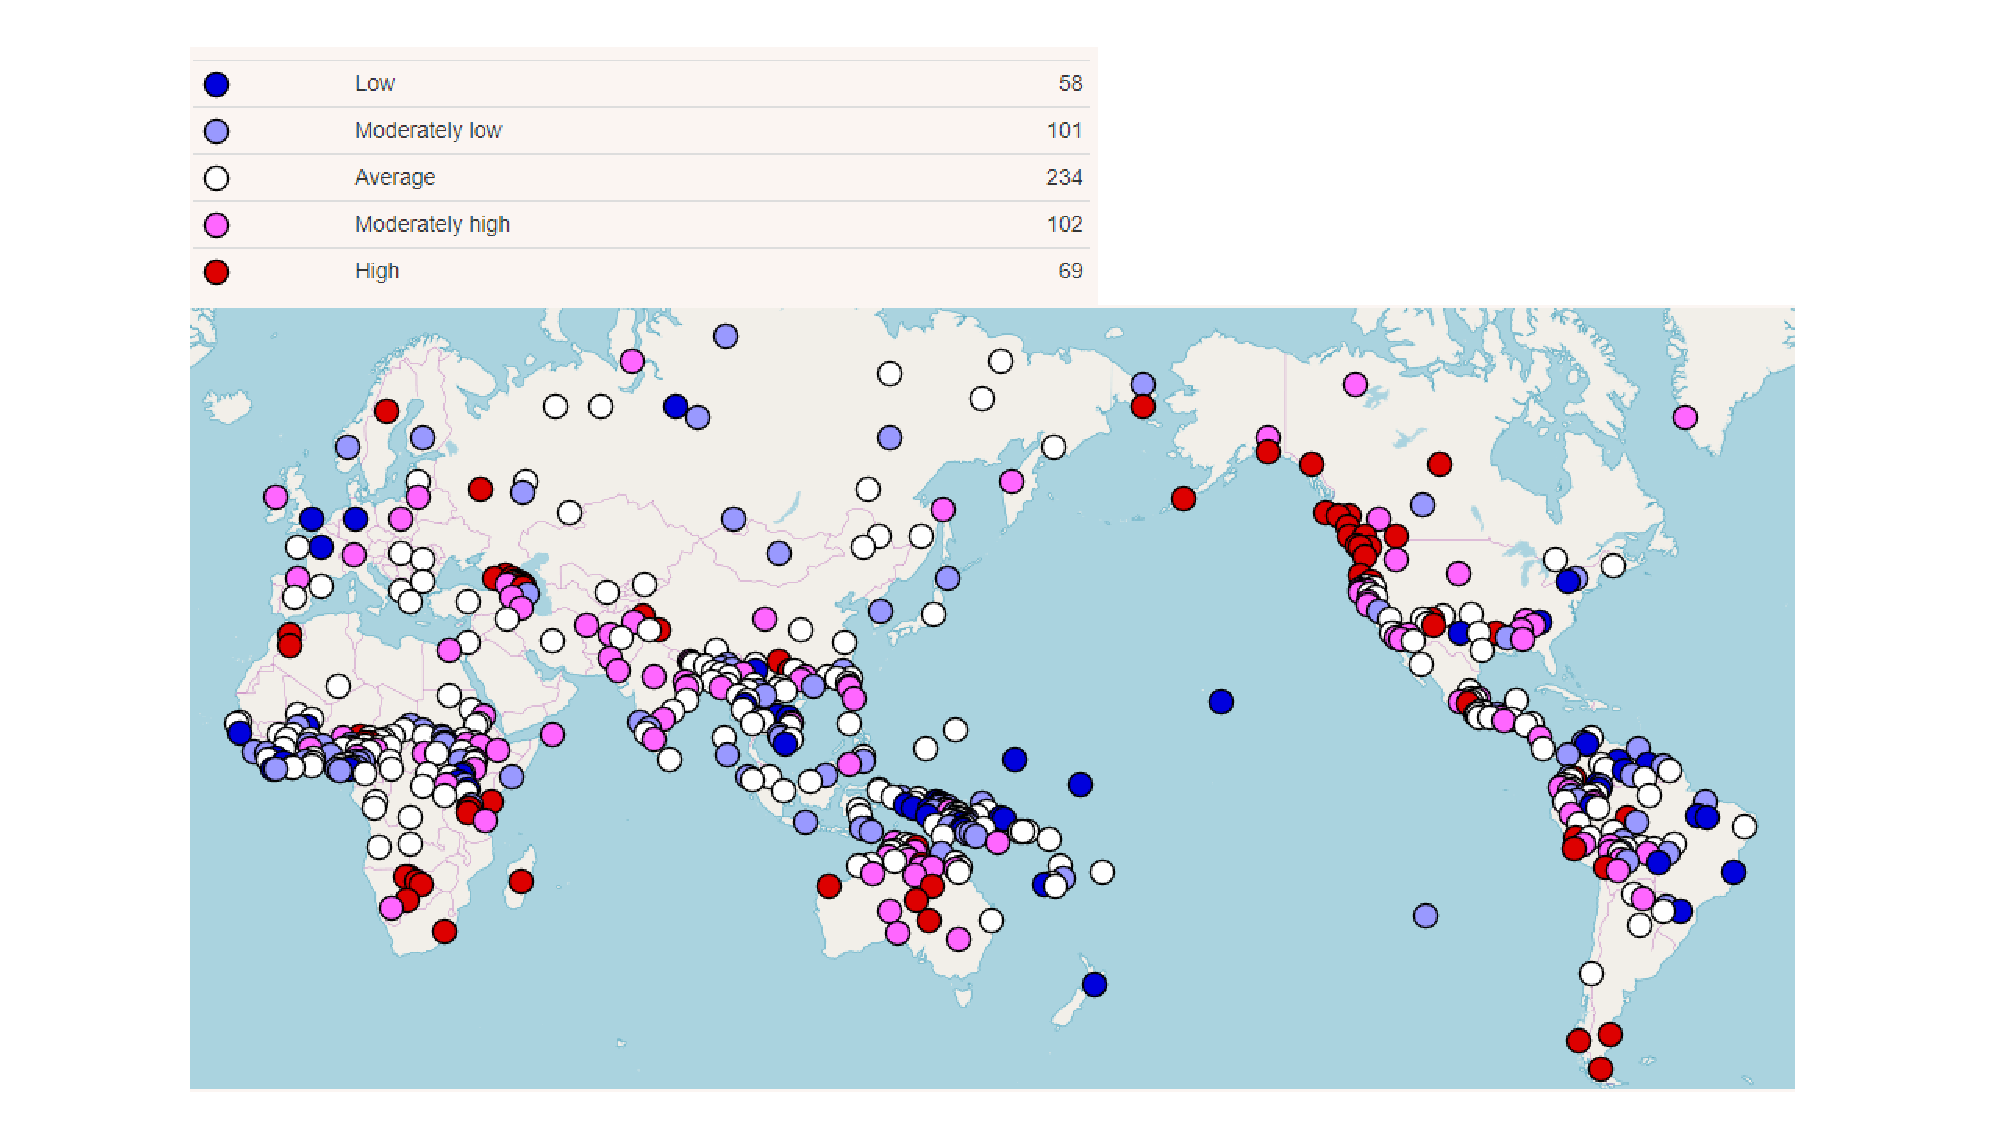
\includegraphics[width = 0.8\linewidth]{figures/WALS_example.pdf}
\caption{Consonant-vowel ratio across sampled languages by WALS. Different colors represent different level of consonant-vowel ratio: blue for low level, light blue for moderately low level, white for average level, magenta for moderately high level and red for high level.}
\label{fig:wals_example}
\end{figure}

First, in figure \ref{fig:wals_example}, the consonant-vowel ratio is used as an example of how phonological patterns are different across world's languages. Higher ratio means there are more consonants and less vowels in that language while lower ratio means the opposite. Take some commonly used languages as examples: English, German and French all have low ratio; Spanish, Persian and Mandarin have average ratio; Russian has high ratio.

\begin{table}[]
\centering
\caption{19 language phonological features summarized by WALS. The last column indicates whether the feature is phonetic or rhythmic feature. For detailed description of each feature, refer to \citep{wals}}
\label{table: wals_feature}
\begin{tabular}{|c|c|}
\hline
Feature name & Phonetic or Rhythmic \\ \hline
Consonant Inventories & Phonetic \\ \hline
Vowel Quality Inventories & Phonetic \\ \hline
Consonant-Vowel Ratio & Rhythmic\tablefootnote{Although Consonant-Vowel Ratio looks like a phonetic feature because it is the ratio of the number of consonants and vowels, most studies regard it as a rhythmic feature \citep{gil1986prosodic}.} \\ \hline
Voicing in Plosives and Fricatives & Phonetic \\ \hline
Voicing and Gaps in Plosive Systems & Phonetic \\ \hline
Uvular Consonants & Phonetic \\ \hline
Glottalized Consonants & Phonetic \\ \hline
Lateral Consonants & Phonetic \\ \hline
The Velar Nasal & Phonetic \\ \hline
Vowel Nasalization & Phonetic \\ \hline
Front Rounded Vowels & Phonetic \\ \hline
Syllable Structure & Rhythmic \\ \hline
Tone & Rhythmic \\ \hline
Fixed Stress Locations & Rhythmic \\ \hline
Weight-Sensitive Stress & Rhythmic \\ \hline
Weight Factors in Weight-Sensitive Stress System & Rhythmic \\ \hline
Rhythm Types & Rhythmic \\ \hline
Absence of Common Consonants & Phonetic \\ \hline
Presence of Uncommon Consonants & Phonetic \\ \hline
\end{tabular}
\end{table}

Next, it is clearer to do differential analysis of different languages with phonological patterns and to illustrate the distance among different languages on phonological feature space. To achieve this, several phonological features pre-summarized by WALS are selected. Based on whether there definitions are segmental or supra-segmental, those features are categorized into phonetic features and rhythmic features. Two groups of features represent language phonological patterns on phonetic space and rhythm space respectively. Table \ref{table: wals_feature} includes those features' names and indicates whether each feature is phonetic or rhythmic\footnote{Downloadable from \url{https://cdstar.shh.mpg.de/bitstreams/EAEA0-7269-77E5-3E10-0/wals_language.csv.zip}}. WALS assigns feature values to languages based on the structural properties of languages that describe one aspect of cross-linguistic diversity. For example, the feature ``Rhythm Types'' has five values: Trochaic (left-hand syllable in the foot is strong), Iambic (right-hand syllable in the foot is strong), Dual (system has both trochaic and iambic feet), Undetermined (no clear foot type) and Absent (no rhythmic stress). Those feature values are stored as a number, usually starting from 1, to represent each categories they belong to. To visualize those languages on a 2-dimensional space, the numeric values of each feature are used. If one feature is not applicable to a language, 0 is used instead. As a result, each language will have a 19-dimensional feature vector representing values of those features in table \ref{table: wals_feature}. Each feature vector is also split into phonetic and rhythmic feature vectors. Since each feature actually indicate a category, to make sure the distances among different categories are the same, one-hot encoding is used to convert the integer feature value to a vector consisting of 0s and 1s. The length of the encoded vector is equal to the number of categories that feature can be. For example, the ``Rhythm Types'' feature has 5 categories. Then, a number of 3 will be encoded as ``00010''. Multidimensional scaling (MDS), which seeks a low-dimensional representation of those feature vectors in which the distances respect well the distances in the original high-dimensional space, is employed to illustrate the 2-dimensional representation of each language in all phonological feature space (as shown in figure \ref{fig:all_mds}), phonetic feature only space (as shown in figure \ref{fig:phonetic_mds}) and rhythmic feature only space (as shown in \ref{fig:rhythmic_mds}) with the encoded language features.

\begin{figure}
\centering
\minipage{0.55\textwidth}
  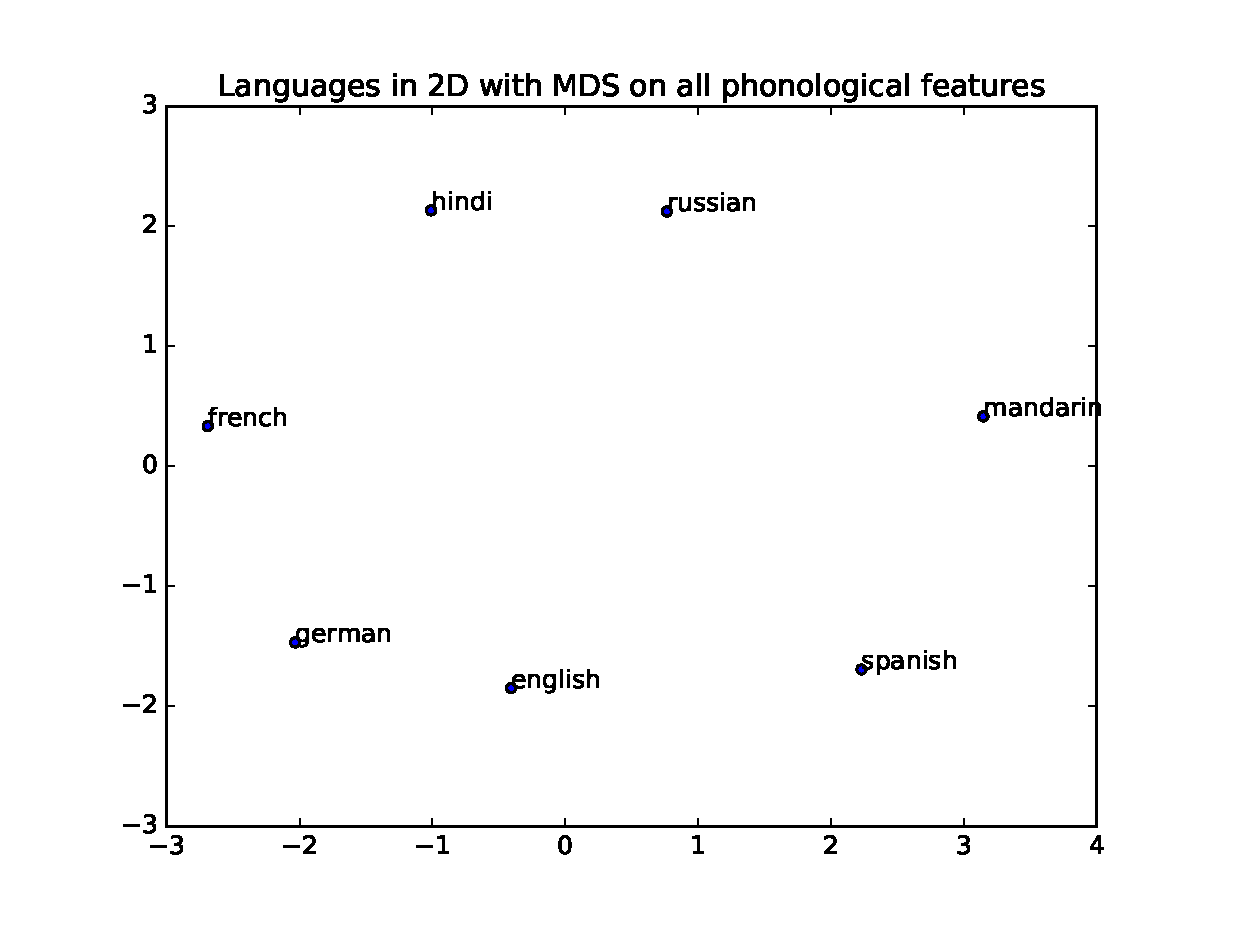
\includegraphics[width=\linewidth]{figures/all_MDS.eps}
  \caption{2D visualization of all features with MDS.}\label{fig:all_mds}
\endminipage\hfill
\\
\minipage{0.55\textwidth}
  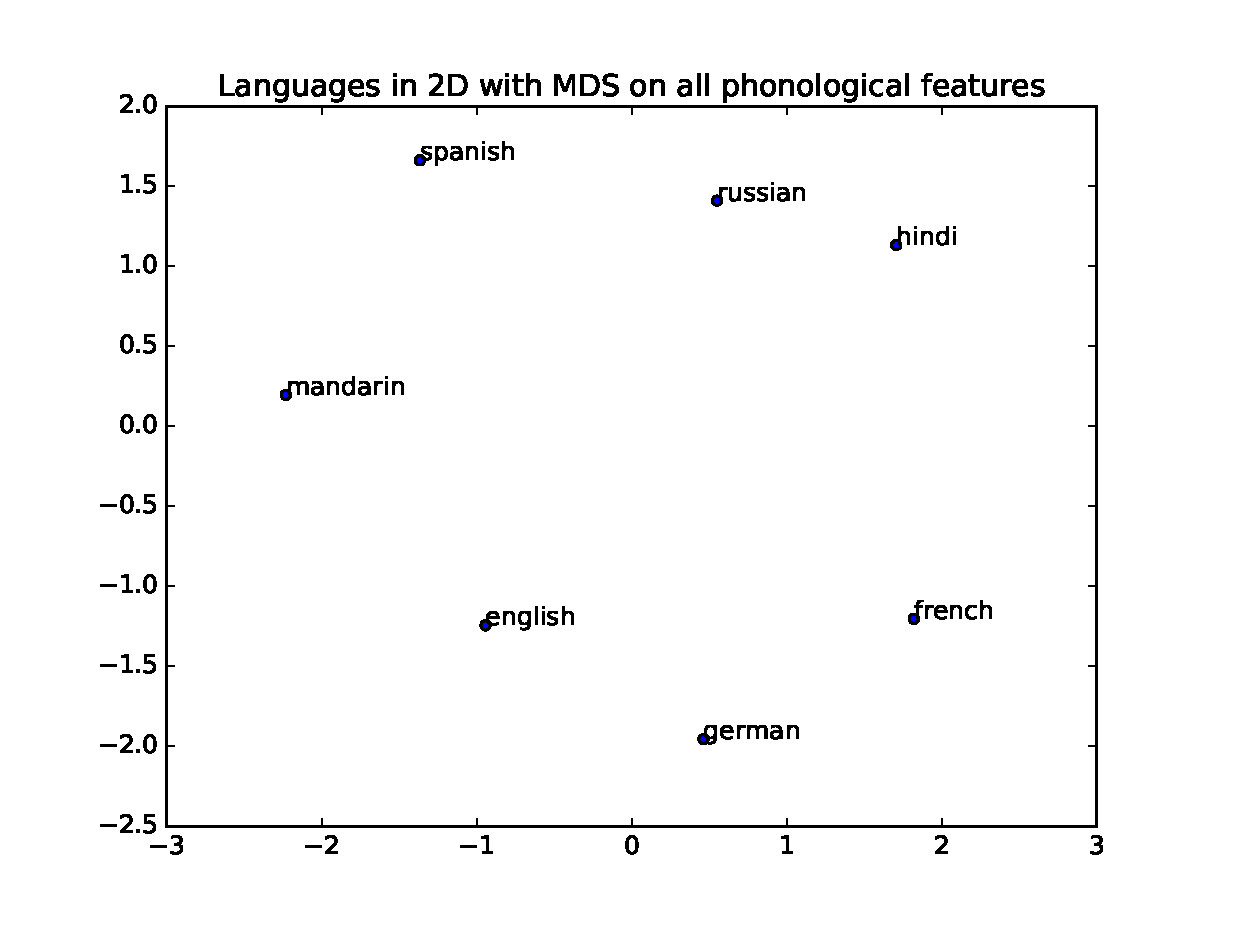
\includegraphics[width=\linewidth]{figures/phono_MDS_wals.eps}
  \caption{2D visualization of phonetic only features with MDS.}\label{fig:phonetic_mds}
\endminipage\hfill
\\
\minipage{0.55\textwidth}%
  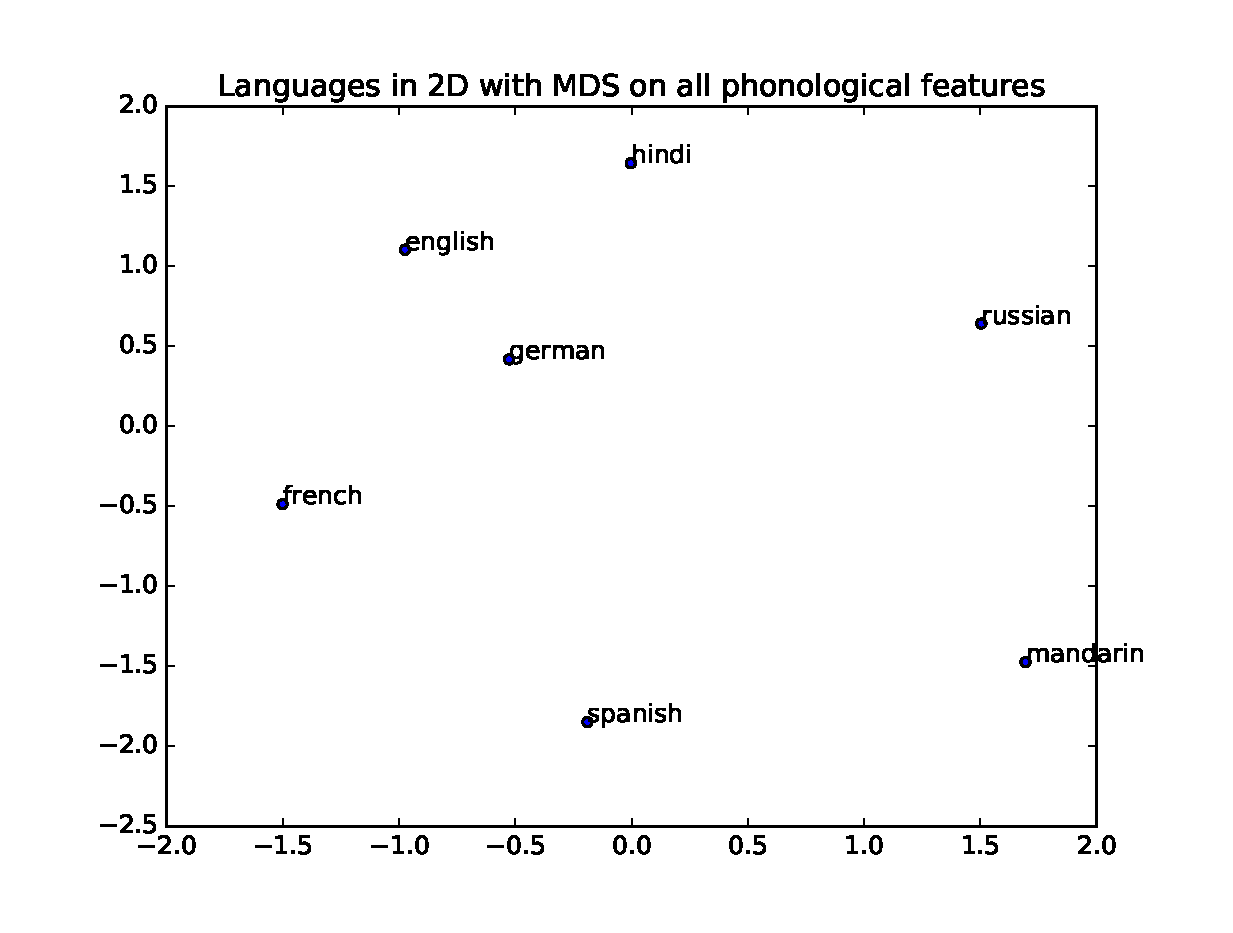
\includegraphics[width=\linewidth]{figures/rhythmic_MDS.eps}
  \caption{2D visualization of rhythmic only features with MDS.}\label{fig:rhythmic_mds}
\endminipage
\end{figure}

Along with the 2-dimensional visualization, normalized pair-wise distance matrices are also shown in table \ref{table:conf_all} for all features, table \ref{table:conf_phonetic} for phonetic features and table \ref{table:conf_rhythmic} for rhythmic features. The pairwise distance between two languages is calculated as follows: count the number of different values for corresponding dimensions of the feature vectors of two languages without one-hot encoding. This will result in a $N \times N$ matrix where N is the number of languages; normalize the matrix by the maximum value in the matrix. From the feature visualization and normalized pair-wise distance matrices, it can be found that English, German and French are relatively close to each other on all three feature space while other languages are relative far from those three languages. If English is regarded as L2, German is closest to English on all features space. Furthermore, German is closer to English on rhythmic space than phonetic space. So is French. However, Mandarin and Spanish are closer to English on phonetic space than rhythmic space. One important question this study wants to investigate is that whether those L1 to L2 distance patterns will manifest in the accented speech perception: how the relative importance of segmental features and supra-segmental features relates to the distance to L2 on phonetic and rhythmic space.

\begin{table}[t]
\centering
\caption{Normalized pairwise distance on all features space.}
\label{table:conf_all}
\resizebox{0.55\columnwidth}{!}{%
\begin{tabular}{|c|c|c|c|c|c|c|c|}
\hline
 & German & Spanish & French & Russian & Hindi & English & Mandarin \\ \hline
German & 0 & 0.92 & 0.33 & 0.67 & 0.67 & 0.33 & 0.83 \\ \hline
Spanish &  & 0 & 0.83 & 0.67 & 0.75 & 0.67 & 0.50 \\ \hline
French &  &  & 0 & 0.67 & 0.58 & 0.58 & 1.00 \\ \hline
Russian &  &  &  & 0 & 0.42 & 0.58 & 0.75 \\ \hline
Hindi &  &  &  &  & 0 & 0.50 & 0.92 \\ \hline
English &  &  &  &  &  & 0 & 0.83 \\ \hline
Mandarin &  &  &  &  &  &  & 0 \\ \hline
\end{tabular}}
\end{table}

\begin{table}[t]
\centering
\caption{Normalized pairwise distance on phonetic features only space.}
\label{table:conf_phonetic}
\resizebox{0.55\columnwidth}{!}{%
\begin{tabular}{|c|c|c|c|c|c|c|c|}
\hline
 & German & Spanish & French & Russian & Hindi & English & Mandarin \\ \hline
German & 0 & 1.00 & 0.29 & 0.71 & 0.86 & 0.43 & 0.71 \\ \hline
Spanish &  & 0 & 1.00 & 0.57 & 0.71 & 0.57 & 0.43 \\ \hline
French &  &  & 0 & 0.71 & 0.57 & 0.71 & 1.00 \\ \hline
Russian &  &  &  & 0 & 0.29 & 0.57 & 0.71 \\ \hline
Hindi &  &  &  &  & 0 & 0.71 & 0.86 \\ \hline
English &  &  &  &  &  & 0 & 0.71 \\ \hline
Mandarin &  &  &  &  &  &  & 0 \\ \hline
\end{tabular}}
\end{table}

\begin{table}[t]
\centering
\caption{Normalized pairwise distance on rhythmic features only space.}
\label{table:conf_rhythmic}
\resizebox{0.55\columnwidth}{!}{%
\begin{tabular}{|c|c|c|c|c|c|c|c|}
\hline
 & German & Spanish & French & Russian & Hindi & English & Mandarin \\ \hline
German & 0 & 0.80 & 0.40 & 0.60 & 0.40 & 0.20 & 1.00 \\ \hline
Spanish &  & 0 & 0.60 & 0.80 & 0.80 & 0.80 & 0.60 \\ \hline
French &  &  & 0 & 0.60 & 0.60 & 0.40 & 1.00 \\ \hline
Russian &  &  &  & 0 & 0.60 & 0.60 & 0.80 \\ \hline
Hindi &  &  &  &  & 0 & 0.20 & 1.00 \\ \hline
English &  &  &  &  &  & 0 & 1.00 \\ \hline
Mandarin &  &  &  &  &  &  & 0 \\ \hline
\end{tabular}}
\end{table}

The previous features are summarized by linguistics on a high systematic level. How those features manifest themselves in the acoustic recordings of different languages? How the languages' differences manifest themselves in the key parameters of acoustic speech signal including intensity, pitch, formants, envelop and so on? Several studies have investigate this and those findings. An early study \citep{parmenter1933experimental} compared the acoustic characteristics between English and French reading speech and showed that pitch is more important as an element of accent than intensity for French speech while intensity is more important for English speech. Also, French speech has more pitch variation than English. Studies in \citep{jongman1989acoustic,bradlow1995comparative,al2005does} investigated the relationship between vowel inventories and vowel space (defined as the two-dimensional area bounded by lines connecting first and second formant frequency coordinates of vowels \citep{fant1973speech}) and concluded that vowel space depends on the size of vowel inventory: the larger the inventory, the bigger the acoustic space. The work by \citep{wagner2003voice} showed that predominant factors in voice quality are different across different languages. In terms of speech rhythm, an influential study in \citep{ramus1999correlates} studied the representation of linguistic speech rhythm in acoustic speech signal. Several acoustic measurements for speech rhythm are proposed to discriminate the rhythm classes of different languages. Those measurements include the percentage of vocalic segment in an utterance ($\%V$), the standard deviation of consonant intervals ($\Delta C$) and the standard deviation of vowel intervals ($\Delta V$). Figure \ref{fig:rhythm_lang} is taken from \citep{ramus1999correlates} to show how $\%V$ and $\Delta C$ can discriminate languages. Based this study, other measurements like variational coefficient of consonant/vowel intervals \citep{dellwo2006rhythm}, pairwise variability index (PVI) of consonant/vowel intervals \citep{grabe2002durational} are also proposed. Those studies that correlate those linguistically summarized phonological language features with acoustic measurements lay the foundation of the methodology used in this study.

\begin{figure}
\centering
\captionsetup{justification=centering}
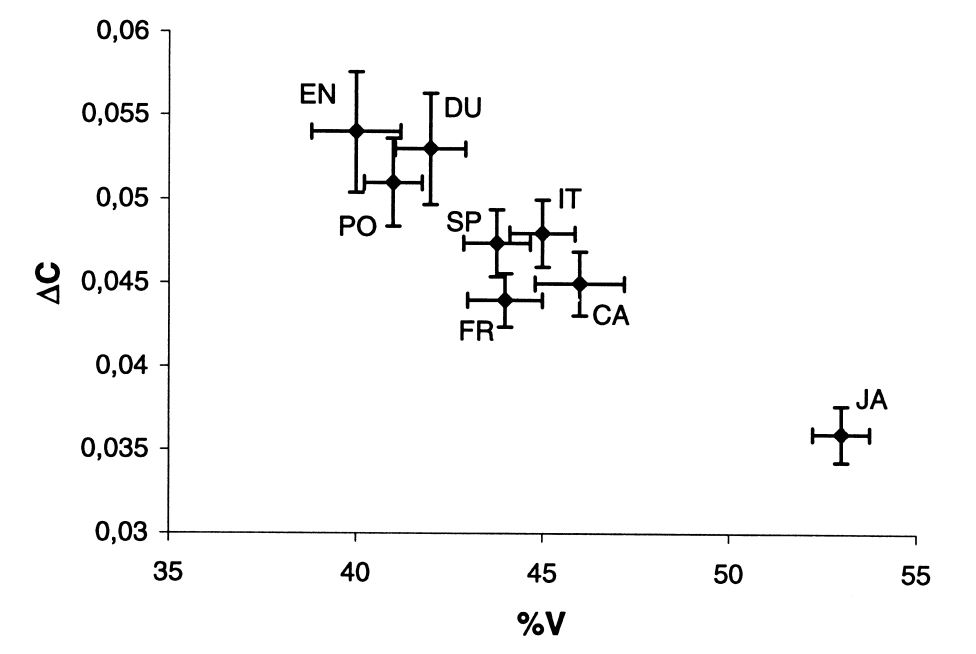
\includegraphics[width = 0.8\linewidth]{figures/ramus_paper.JPG}
\caption{Distribution of languages over the ($\%V$, $\Delta C$) plane. EN: English, PO: Polish, DU: Dutch, SP: Spanish, IT: Italian, FR: French, CA: Catalan, JA: Japanese. Taken from \citep{ramus1999correlates}}
\label{fig:rhythm_lang}
\end{figure}

\section{L2 learning theories}

In the literature, there is a huge body of research on the L1 acquisition: how a child acquires a complicated linguistic system including different levels of information without explicit guidance. As summarized by \cite{chang2010first}, those studies both the effect of an innately endowed Universal Grammar and the effect of the timely input on L1 acquisition. Similar research track has been borrowed to study the L2 learning theories: investigating both the influence of already built linguistic system (L1) and some universal effect that are independent of the already built linguistic system. It has been shown that while moving toward to the target L2 linguistic system, L2 learners usually show trackable difference from the implementation of native L2 speakers, which is attributed to the influence of the learner's L1. In terms of phonology, this is where the perceived foreign accent comes from. Considering L1 interference mechanism, i.e., the phonological knowledge transfer from L1 to L2, are focused by the majority of the literature and is more related to the current study, in this chapter research body on phonetic acquisition will be reviewed. Specifically, some well-established L2 learning theories focusing on the accented phoneme production will be introduced first. Then, studies on speech prosody acquisition in L2 learning will be covered. Last subsection will focus on the role of L1 in L2 learning and elaborate more on the L1's interference in L2 learning.

\subsection{Phonetic acquisition}

There have been studies trying to explain the origin of the foreign accent in producing L2 phonemes. The critical period hypothesis from L1 acquisition was extended to L2 acquisition, positing that a critical age or period after which L2 speech production could not be native like because of the neurological maturation \citep{long1990maturational}. Other studies assumes the failure to acquire native-like production of L2 is caused by factors like inaccurate perception of L2 sounds, inadequate phonetic input, insufficient motivation, psychological reasons and incorrect L2 habit because of incorrect instructions \citep{flege1988production}. Although all these observations partly show evidence of the origin of the foreign accent, they fail to explain the L2 learning process in a systematic way and how L2 learning is different from L1 acquisition. Nonetheless, there is consensus achieved by the community that the earlier one starts to learn a L2 the better\footnote{There is still some outliers found by researchers, for example it was reported that both early L2 learners still failed to achieve native-like production while late L2 learners did \citep{flege1995second}}.

Developed by \cite{flege1995second}, the speech learning model (SLM) are the most influential study in L2 speech learning literature. Different from the critical period hypothesis, SLM assumes that the phonetic systems used in the production and perception of vowels and consonants is active during the whole life span. It functions like a dynamic system that can encode all phonetic input. As mentioned in \citep{flege1995second}, ``the phonetic systems reorganize in response to sounds encountered in an L2 through the addition of new phonetic categories, or through the modification of old ones''. L1 and L2 phonetic categories exist in a shared system and there is motivation to keep them distinct from each other. This indicates that the formation of the phonetic system of accented speech is based on the L2 learner's already-established L1 phonetic system. To explain this age-related L2 learning process, SLM has 4 postulates and 7 hypotheses. The 4 postulates \citep{flege1995second} are:

\begin{enumerate}
\item The mechanisms and processes used in learning the L1 sound system, including category formation, remain intact over the life span, and can be applied to L2 learning.
\item Language-specific aspects of speech sounds are specified in long-term memory representations called phonetic categories.
\item Phonetic categories established in childhood for L1 sounds evolve over the life span to reflect the properties of all L1 or L2 phones identified as a realization of each category.
\item Bilinguals strive to maintain contrast between L1 and L2 phonetic categories, which exist in a common phonological space.
\end{enumerate}

The 7 hypotheses are based on those 4 postulates and on evidences from data analysis in previous studies on speech production of l2 learners. Next, each hypothesis together with evidences and predicts will be introduced (most can be found in the review paper \cite{flege1995second}).

\textbf{Hypothesis 1:} sounds in the L1 and L2 are related perceptually to one another at a position-sensitive allophonic level, rater than at a more abstract phonemic level. L2 learners will perceive positional allophones in the L2 to the most similar positionally defined allophone in the L1. Studies have shown that it is easier for L2 learners to produce and perceive certain allophones of English phonemes than others. Native Japanese speakers are taken as example. It is hard for native Japanese speakers producing and perceiving English /\textipa{l}/ and /\textipa{r}/ because in Japanese there is only one liquid while English has two. Thus, the contrast between /\textipa{l}/ and /\textipa{r}/ is difficult to attain. However, it has been found that the production accuracy of these two liquids depends on phonological environments. In \citep{strange1992learning}, the authors showed that native Japanese learners of English characteristically perceive and produce English liquids more accurately in word-final than word-initial position. They attributed this to that the acoustic difference between English /\textipa{l}/and /\textipa{r}/ is more robust in final than initial position \citep{sheldon1982acquisition}. This indicates the position-sensitive relationship between L1 and L2 sounds in allpphonic level.

\textbf{Hypothesis 2:} a new phonetic category can be established for an L2 sound that differs phonetically from the closest L1 sound if bilinguals discern at least some of the phonetic differences between the L1 and L2 sounds. The likelihood of the formation of a new phonetic category increases with the dissimilarity between an L2 sound and the closet L1 sound. Several studies have shown that when a novel phoneme (not exist in L1 or very different from L1 phonemes) is encountered, L2 learners can usually produce it accurately. In \citep{flege1987production}, the authors found that native English speakers can produce the French vowel /\textipa{y}/, a vowel that does not exist in English, relatively accurately compared to native French speakers. \cite{flege1997english} further showed that native Dutch speakers can produce the English vowel /\textipa{\ae}/ accurately and same results were found in another study on German speakers \citep{flege1997perception}. Those findings suggest that if the phonetic differences between the L2 sound to the closet L1 sound exist obviously, the production of the L2 sound can be produced accurately.

\begin{figure}
\centering
\captionsetup{justification=centering}
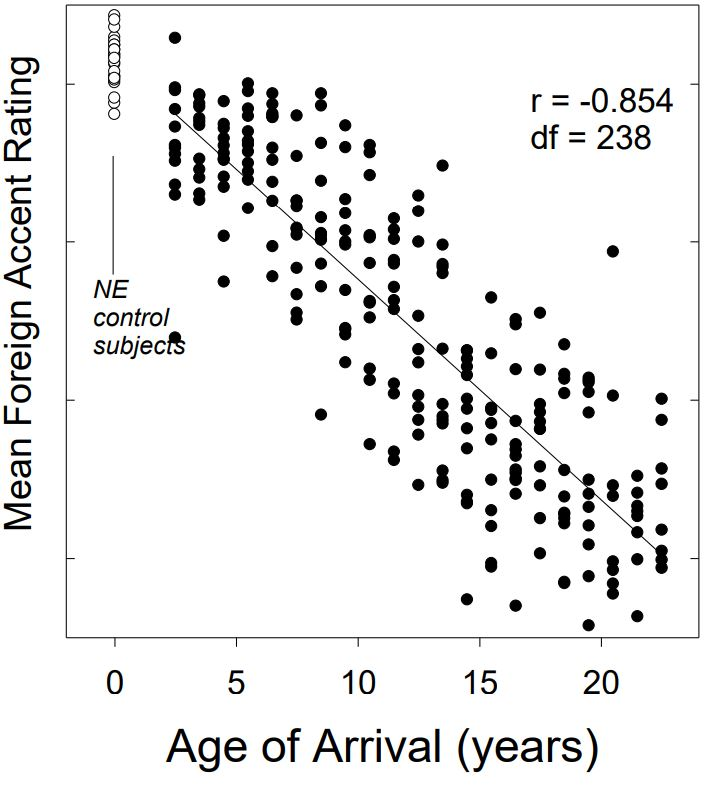
\includegraphics[width = 0.8\linewidth]{figures/accentedness_AOA.JPG}
\caption{The mean foreign accent ratings (Y-axis) of English sentences spoken by native Korean immigrants to US. X-axis represents the age of arrival. Taken from \citep{flege1999native}.}
\label{fig:accent_example}
\end{figure}

\textbf{Hypothesis 3:} The likelihood of phonetic differences between L1 and L2 sounds, and between L2 sounds that are noncontrastive in the L1, being discerned decreases as the age of learning increases. For example, the study in \citep{butcher1978influence} showed that the perceived distance between /\textipa{ae}/ in English and /\textepsilon/ in German is greater for German children than adults. \cite{weiher1975lautwahrnehmung} also showed that German adults but not children have difficulty discriminating /\textipa{ae}/ in English and /\textepsilon/. Based on this hypothesis, it can be predicted that with the increasing of the age of learning, more sounds in L2 will be inaccurately produced. Thus, a linear relationship between perceived accentedness and age of learning is shown in figure \ref{fig:accent_example}, in contrast to the sharp discontinuity in the L2 pronunciation ability suggested by the critical period hypothesis.

\textbf{Hypothesis 4:} Category formation for an L2 sound may be blocked by the mechanism of equivalence classification. When the block occurs, speakers tend to use a single phonetic category to process perceptually similar L1 and L2 sounds, resulting in inaccurate production of L2 sounds. The study by \cite{flege1987production} showed that French learners who are native American English speakers produce the French phoneme /\textipa{u}/ with second formant ($F_2$) values higher than native French speakers, which is influenced by the high-$F_2$ /\textipa{u}/ in English. \cite{chang2008phonetic} also reported that native American English speakers also produce Mandarin phoneme /\textipa{u}/ with higher $F_2$. \cite{flege1987production} also showed that native English speakers produce French voiceless stops with too long voice onset times (VOTs), under influence from the long-lag VOT of English voiceless stops.

\textbf{Hypothesis 5:} The phonetic category established for L2 sounds by a bilingual may differ from a monolingual's if: 1) the bilingual's category deviates from an L2 category to maintain phonetic contrast between categories in a common L1-L2 phonological space; or 2) the bilingual's representation is based on different features, or feature weights, than a monolingual's. The evidence can be found in the study by \cite{munro1993productions} where the authors showed that even experienced L2 English speakers who are native Arabic speakers produce vowels that are considered to have accent. According to the study, the accentedness was due to non-native production of duration differences between tense and lax English vowels. They suggest that in this case the L2 tense and lax categories might have been interpreted as long and short categories, which exist in Arabic. The evidence of the second point is shown in \citep{munro1996effects}. This study showed that English learners with Italian as native language can not produce accurate phoneme /\textrhookschwa/, although those learners started to speak English at their ten years age and were rated to have very mild foreign accent. The authors considered he reason to be related to the retroflex feature that is used to discriminate from other English vowels but not exist in Italian.

\textbf{Hypothesis 7:} The production of a sound eventually corresponds to the properties represented in its phonetic category representation. This hypothesis can be regarded as the result of hypothesis 2, 4 and 5, stating the L2 sound will eventually be produced as specified in phonetic category representation. If the presentation matches the category for native L2 speakers, then the L2 sound can be produced accurately; if new phonetic category for L2 sounds is not formed or different from monolingual's, there will be inaccurate pronunciation.

To summarize, SLM claims the age of learning has significant on second language learning: this can be seen from those hypotheses that age of learning directly influence the formation of phonetic categories to produce L2 sounds. Also, pre-established L1 phonetic categories will affect the way L2 sounds are perceived  and thus will also influence the formation of phonetic categories. If similar sounds in L2 are too close to sounds in l1, then equivalence classification will use the same phonetic category to produce the similar sounds, resulting in perceivable inaccurate pronunciation for L2 native speakers. Sometimes, phonetic categories built for novel L2 sounds can still be different from native's due to the dissimilation occurs between L1 and L2 phonetic categories to maintain phonetic contrast between categories in a common L1-L2 phonological space. SLM mainly deals with phonetic acquistion, i.e. the segmental accuracy of L2 production. However, a lot of studies have shown that inaccurate supra-segmental productions can also result in perceivable foreign accent \citep{rognoni2013testing,winters2013perceived}. In the next subsection, speech prosody acquisition in the literature will be reviewed to reveal the mechanism L2 learners use to achieve native-like productions of speech prosody.



\subsection{Prosody acquisition}

In the previous subsection, fundamental studies on L2 learning are reviewed. It also can be found that these studies mainly focus on phonetic part in terms of the whole phonological system. Although the study by \cite{munro1993productions} investigated the durations of tense and lax English vowels produced by native Arabic speakers and durations of vowels are related to speech prosody \citep{ramus1999correlates}, most analysis in these studies only deals with pronunciation of specific phonemes; some even use isolated phonemes or words \citep{flege1987production}. Whether the theories proposed by these studies can be applied to prosodic inaccuracy of non-native L2 speech is still questionable \citep{rasier2007prosodic}. On the other hand, a review survey by \cite{gut2009non} showed that for all studies on L2 speech learning from 1969 to 2008, L2 intonation was only investigated in nine studies and L2 speech rhythm was only investigated in four studies \citep{mennen2004bi,altmann2006perception,rasier2007prosodic,lin2008interlanguage}. This indicates that the speech prosody in L2 speech is quite underexplored. In this subsection, literature on acquisition of speech prosody during L2 learning will be reviewed.

The study by \cite{mennen2004bi} investigated how the Dutch non-native speakers of Greek realize the timing of a phonologically identical rise: nonfinal or prenuclear rises. This phonological property was realized differently by native Dutch and native Greek speakers: 1) at different time; The peak in the rise appeared earlier in Dutch than in Greek. 2) The peak time in Dutch depends on the the phonological length of the vowel of accented syllable while Greek did not. By analyzing the timing patterns of the rise using five native Dutch speakers speaking Greek, the authors concluded that there existed a bi-directional interference in the realization of the rising accent: the L1 Dutch affected the realization in Greek and the L2 Greek also affected the realization in Dutch. The dissertation by \cite{altmann2006perception} studied the perception and production of advanced learners of English with different L1 backgrounds (Arabic, Chinese, French, Japanese, Korean, Spanish, Turkish) to investigate the effect of L1 stress properties on the L2 acquisition of primary word stress. The results showed that native speakers of L1s with predictable stress felt difficult to locate the stress in English while they were able to produce the correct stress patterns; native speakers of L1s without word-level stress or predictable stress performed well in stress perception but had difficulties in stress production. These results are kind of against the SLM: good perception of stress patterns does not mean good production. In the study by \cite{rasier2007prosodic}, the authors reviewed the prosody acquisition of L1 learning and proposed a general framework to study the prosody transfer from L1 to L2 in L2 learning. The model was tested in a study of accent in L2 Dutch proposed by native French speakers and L2 French produced by native Dutch speakers. Their results showed that the difference between French and Dutch on accent placement influenced the acquisition process of accentuation. The ``Markedness'' proposed in \cite{eckman1977markedness} is an important factor in predicting and explaining learning difficulties in L2 prosody learning.

The previous studies mainly focus on stress and accent. The following introduced studies in this paragraph investigate the prosodic properties acquisition in terms of duration and duration variability measurements which have been shown to able to discriminate among languages within different rhythmic classes \cite{ramus1999correlates,grabe2002durational}. Those measurements include:

\begin{enumerate}
\item $\Delta V$: the standard deviation of vocalic intervals
\item $\Delta C$: the standard deviation of consonantal intervals
\item $\%V$: percentage of vocalic intervals in the sentence
\item $VarcoV$: the standard deviation of vocalic intervals divided by the mean vocalic interval duration and multiplied by 100
\item $VarcoC$: the standard deviation of consonantal intervals divided by the mean consonantal interval duration and multiplied by 100
\item $nPVI-V$: the normalized PVI for vocalic intervals
\item $rPVI-C$: the raw PVI for consonantal intervals
\end{enumerate}

The study in \citep{stockmal2005measures} examined speech rhythm of the Latvian produced by native Russian learners. In their result, there was no clean increase in vocalic variability between experienced and low-level learners, in spite that Latvian is significantly less stress-timed than Russian. They concluded that even if the learner's L1 is stress-timed and has higher vocalic variability, at the early stage of acquisition the accented speech can still match the L2 in terms of lower vocalic variability. They also found that the consonantal duration variability increased significantly during L2 acquisition and attributed to the difficulties of consonants articulation. \cite{white2007calibrating} used all the seven rhythmic measurements and showed that those measurements were able to separate stress-timed English and Dutch and syllable-timed Spanish and French. They also applied the measurement to quantifying the influence of L1 on L2 rhythm acquisition when switching between stress-timed and syllable-timed. In the experiment consisting of native Spanish subjective speaking English and native English speakers speaking Spanish, it was found that the $VarcoV$, $nPVI-V$ and $rPVI-C$ were in the intermediate stage during the transfer from L1 to L2, indicating clearly the influence of L1 rhythm on l2. In the experiment consisting of native Dutch subjective speaking English and native English speakers speaking Dutch (both the two languages are stress-timed), it was found that there was no clear influence of L1. The authors believed that if L1 and L2 are already rhythmic similar, the L2 learners tend to make little accommodation and use their L1 rhythmic patterns. \cite{lin2008interlanguage} examines the accented English speech produced by native Mandarin speakers in terms of four measurements of speech rhythm: $\%V$, $\Delta C$, $rPVI-C$ and $nPVI-V$. With the reading and conversational recordings of 6 subjects, the authors showed that the value of $\%V$ of Mandarin accented English is in the middle of the value of native English speakers (lower) and native Mandarin speakers (higher). They explained that this indicated the L1 rhythm patterns had an effect on L2 rhythm patterns in terms of $\%V$; The average nPVI value was very close to native English speakers and the authors attributed this to that those Mandarin subjects mastered the vocalic variability. However, the average values of other two measurements are way higher than native English speakers. The authors believed it was because the consonantal duration patterns were much harder to acquire for Mandarin speakers when speaking English. Similar results were also reported in \citep{kawase2016influence} where the rhythmic acquisition of native Japanese (mora-timed) learners of English (stress-timed) was studied. \cite{li2014l2} conducted experiments on durational variation in L2 English productions by: L1 Mandarin learners and L1 German learners compared to native control values in English. The results showed that the L1 groups followed comparable developmental paths in their acquisition of vocalic variability and accentual lengthening. However, the two L1 groups diverged in the proportion of vocalic materials in their L2 utterances and indicated L2 acquisition patterns that are consistent with direct transfer from the L1. Thus, they claimed that there was a multisystemic model of L2 rhythm acquisition and both transferred L1 knowledge and universal effects independent of L1 played a role. \cite{ordin2015acquisition} did similar experiments to examine the differences in durational variability (several rhythmic measurements) between proficiency levels in L2 English spoken by French and German learners. They found that speech rhythm in L2 English learners in both groups developed from more syllable-timed toward more stress-timed patterns irrespective of the L1 had similar rhythmic patterns. However, they also showed that there were differences between the German and French groups: German learners achieved a degree of durational variability typical of the target language while French learners exhibited lower variability than native speakers.

Recently there are also some studies investigating the relative importance of suprasegmental measurements to accentedness perception compared to segmental measurements. In (\cite{rognoni2013testing}, \cite{winters2013perceived}), the authors transplanted the prosody measurements (F0 and duration) between native English speech and accented English speech in both directions to analyze the relative importance of segmental and suprasegmental features' contribution to accentedness perception. They both found that though prosodic features contribute to the perception of accentedness, segmental features is more important than suprasegmental features. The study in (\cite{polyanskaya2016relative}) applied the similar transplantation method to speaking rate and speech rhythm and they drew the conclusion that speech rhythm contributed more to accentedness perception than speaking rate. A following study by \cite{van2017l1} further investigated the interplay of different rhythmic measurements including intonation, rhythm and speech rate and they found that while all measurements contributed to accentedness perception, intonation contributed the most for Dutch learners. However, all of these studies only did the transplantation on one foreign language (Italian, German, French or Spanish) and the contrastive information among different L1s was ignored. Another work by \cite{saito2016second} studied the relative contribution of segmental and supra-segmental to accentedness at different proficiency levels through regression analysis. Their subjects were Japanese who were learning English at different stages.

The prosody acquisition during L2 learning can be summarized as following:
\begin{enumerate}
\item Although there are evidences showing that some universal effects exist in prosody acquisition, most studies report the influence of the L1 on the prosody production of L2. This is similar to the phonetic acquisition.
\item Not all of the prosodic properties depend on the L1 during speech prosody acquisition, in spite that those properties can well discriminate between L1 and L2.
\item When the contrastive information between L1 and L2 can be well perceived, the prosody acquisition follow a path from L1 prosody features to L2 prosody features; when the contrastive information between L1 and L2 is not well perceived or the L1 and L2 prosodic patterns are very close, there is no clear sign of the influence of L1 prosodic patterns.
\end{enumerate}


\subsection{Role of L1 in L2 learning}

In last two subsections, studies dealing with the phonological system acquisition during L2 learning are introduced. However, a lot of studies only investigate one pair of L1 and L2: a one to one mapping, which can not reveal whether the difference of L1s can be projected to the accented L2 speech. Combining the acquisition of L2 in both segmental and supra-segmental perspective, it can be found that different L1s can result in different developments of L2 acquisition. A following question is that how the segmental and supra-segmental production developments of L2 learners from different L1s are different. Since different L1s have very different segmental and supra-segmental characteristics compared to L2, L2 learners from different L1s should undergo different procedures in both segmental and supra-segmental feature space as in the findings by \cite{ordin2015acquisition} although there exist some universal effects. In this subsection, a brief introduction of studies examining multiple L1s and one or multiple L2s are reviewed.
\cite{arslan1997study} calculated four temporal measurements: word-final stop closure duration, VOT, average voicing duration and word duration across three L1 accents: German, Mandarin and Turkey for a set of English words (``target'', ``teeth'', ``catch'', ``communication'') which include a stop consonant in the initial position. While word-final stop closure duration was found to be most discriminative among accents, different accents showed very different patterns in terms of the four measurements. English words with Mandarin accents are the most different from native produced words. German and Turkey speakers are relatively closer to native produced words compared to Mandarin. \cite{mccullough2013perceived} investigated the correlation between different segmental measurements in non-native speech and the perceived accentedness. Speakers from different L1 backgrounds (Hindi, Mandarin and Korean) were rated and analyzed based on their produced English speech. They showed that Hindi has the strongest accent compared to Mandarin and Korean speakers. Analysis of measurements including VOT, vowel quality (measured by F1 and F2 of vowel), vowel durations and F0 differences indicated that non-native speech produced by Hindi speakers showed clear difference compared to Mandarin and Korean speakers while Mandarin and Korean speakers had similar pattern. For supra-segmental measurements, \cite{ramus1999correlates} studied the rhythmic properties across eight languages (English, Polish, Dutch, French, Spanish, Italian, Catalan and Japanese) and applied acoustical rhythmic measurements to language discrimination. They plotted these eight languages on a three dimensional rhythmic space consisting of 1) the proportion of vocal intervals within the sentence. 2) the standard deviation of the duration of vocalic intervals within each sentence 3) the standard deviation of the duration of consonantal intervals within each sentence. The results indicated that there may be more to speech rhythm than just the classification of stress-, syllable and more-timed languages. Also, the difference among different L1s was very obvious. This study inspired the work by \cite{white2007calibrating} and \cite{lai2013applying} where the authors applied similar acoustic analysis of the rhythm properties of both reading and spontaneous L2 speech. \cite{white2007calibrating} applied similar acoustical rhythmic measurements to quantifying the influence of L1 on L2 rhythm. They expected that speakers switching ``rhythm class (stress-timed or syllable timed)'' should show rhythm scores different from both their native and target languages. They found that the standard deviation of vocalic interval duration divided by the mean vocalic interval duration offered the most discriminative analysis of L1, L2 and L1 accented L2, which suggests L1 accented L2 is like an intermediate stage during the transfer from L1 to L2 and speakers with different L1 backgrounds show differences in their accented L2 speech in terms of these rhythmic features. While previous study used reading speech as material, the work by \cite{lai2013applying} investigates the rhythmic measurements of spontaneous L2 speech produced by speakers from different L1 backgrounds. TOEFL Practice Online assessment of 239 speakers from 50 L1 backgrounds was used as speech material. They compared the rhythmic properties of accented L2 speech with the study by \cite{ramus1999correlates} and showed the difference between rhythmic properties of L1 speech and L1 accented L2 speech and also the difference between rhythmic properties of reading and spontaneous accented L2 speech. However, the different rhythmic properties of different L1s were mostly kept in the L1 accented L2 speech.

It can be concluded that in the phonological space of languages, at least on some dimensions (including both segmental and supra-segmental dimensions) L2 learners from different L1 backgrounds follow an speech acquisition path which starts from their L1s and goes towards the target L2. On the path, the L2 speech produced by different L1 learners still show differences that depend on the difference in L1s.

\section{Computational model of accentedness perception}
\label{sec:com_model}

Previous sections reviewed the language differences, second language acquisition of both segmental and supra-segmental phonological properties and how different L1s will result in different development path in L2 learning. This section deals with the learning outcome: accentedness, which is usually defined as the degree of perceived foreign accent. Specially, this section focuses on how accentedness is related to acoustic characteristics of accented speech and whether the accentedness of a speaker can be predicted with computational models given produced accented speech. Furthermore, investigating the relationship between perceived accentedness and acoustic measurements is also a commonly used methodology in L2 learning studies as shown in \citep{ordin2015acquisition,saito2016second}.

Huge amount of studies have been done to investigate the relationship between perceived accentedness and acoustic information such as segmental and suprasegmental measurements and these studies lay the foundation of computational models for accentedness perception. Segmental features measured in short time period, including voice onset time (VOT, defined as the duration between the release of a consonant and the onset of voicing )\citep{lisker1964cross,mccullough2013perceived,mccullough2013perceived}, pronunciation of vowels and consonants \citep{flege1995second,deterding2006pronunciation,sangwan2012automatic}, vowel quality, vowel duration, short-time F0 and harmonics  \citep{mccullough2013acoustic, mccullough2013perceived}, have been shown to contribute significantly to the perception of accentedness. Suprasegmental measurements are also found to be very important to accentedness perception. For example, in  \citep{hardman2014accentedness} the authors investigated the interlanguage match effect of Mandarin-accented English. They found that Mandarin accent had a large negative effect on intelligibility, but the talker accuracy was still high. They considered that low intelligibility was due to a combination of the segmental variation and its misalignment with higher levels of prosody. This means accented speech can be segmentally close to native speech but still results in low intelligibility and high accentedness score due to suprasegmental mismatch. The study by \cite{munro2001modeling, mok2008comparing, kang2010relative} found that suprasegmental measurements such as speaking rate, consonantal/vocalic/syllabic durations, pauses, stress and pitch range of non-native L2 speakers also contribute to the perception of accentedness. How to convert those measurements (Although some of them are computed automatically, most are measured with human labor) in previously introduced studies to acoustic features that can be computed automatically from acoustic signal is the main goal of a computation model for accentedness perception.

Those studies in phonological linguistics have inspired research on computational models for accentedness perception. In the field of computer-assisted pronunciation training (CAPT) and computer-aided language learning (CALL), which has been proved to be able to improve language learning especially word pronunciation \citep{neri2008effectiveness}, many studies investigated improving second language learning and education using computer based accentedness evaluation systems. The goal of automatic accentedness evaluation is to build a statistical machine learning model that predicts the accentedness score of non-native speakers which is supposed to be highly correlated with humans' rating of accentedness score. Acoustic features that can represent the segmental and suprasegmental measurements of accentedness speech are extracted in an automatic way and the evaluation model is responsible for learning the mapping from acoustic features to accentedness score in a supervised learning way. Some studies only focus on pronunciation part of non-native L2 speech while some recent work also includes suprasegmental features.

The first work that aims to develop computer based systems for language learning instruction was conducted in Speech Technology and Research Laboratory at SRI International. Their early pronunciation scoring systems (\cite{bernstein1990automatic}) were designed as text-dependent, which means nonnative speakers must read fixed words or sentences. Text-dependency makes these systems very hard to be used for real language training and evaluation. Their following work focused on text-independent system. The corpus they developed consisted of 100 native French speakers from Paris and 100 American students speaking French. Nonnative French speakers were asked to read designed speech materials including common sentences, newspaper sentences and imitated speech after listening to a native reading the same sentence. Nonnative speakers were rated by language experts on a 1-5 (unintelligible to native quality) scale. The task was to automatically grade the pronunciation performance of nonnative speakers. In (\cite{neumeyer1996automatic}), an automatic pronunciation scoring system was proposed based on an ASR system. First, nonnative speech was segmented using the alignments provided by the ASR system. Four scores were calculated including Hidden Markov Model (HMM) log-likelihood score on each segment, phone classification scores on each segment, segment duration scores calculated by log probability of a phone duration model trained with native speakers, and time scores calculated by averaged and normalized time between syllables. Correlation with human raters showed that segment duration scores provided the highest correlation (sentence level: 0.46, speaker level: 0.74). In their following work, improvement was reported, for example sentence level correlation was improved to 0.50 and speaker level correlation was improved to 0.88 by using average phone segment posterior probabilities, which was calculated by frame-based phone posterior probability. And using score combination (input to linear or nonlinear regression models), sentence level correlation was lifted to 0.62 (\cite{franco1997automatic}). This line of research was extended to assessing pronunciation quality on individual phone segment using the same database (\cite{kim1997automatic}). Listeners were asked to only rate certain segments and same scores were calculated on each segment. Still, log-posterior probability scores provided the highest correlation. The overall speaker level correlation was 0.88. It was also found that human-machine correlation was higher than human-human correlation on both phone segment level and speaker level. A summarization and extension of their previous work on pronunciation scoring was given in (\cite{xi2010eduspeak}). In this research, Spanish was the L2 speech and Spanish learners are native American English speakers. They found word duration scores provided better results than phone duration scores.

In (\cite{sangwan2012automatic}), the authors proposed a automatic accent analysis system of Mandarin accented English using phonological features. With a trained HMM based phonological feature classification system, they built two Markov Models to capture the dynamics of phonological features for both American English speech and Mandarin-accented English. State transitions and state durations of phonological features were believed to carry very important accent-related information. For a given English word produced by a Mandarin speaker, accentedness was represented by delta log-likelihood that is calculated by the log-likelihood of the two trained phonological features Markov models. The accentedness indicator was on a scale from -1 to +1 (from non-native like to native like). Through experiments on CU-Accent corpus (\cite{angkititrakul2006advances}), a correlation of 0.8 was reported between human assigned scores and scores provided by the proposed system. The authors in (\cite{william2013automatic}) proposed a new algorithm for automatic accentedness evaluation. The system had two parts. In the alignment part, speech utterance is processed using a Weighted Finite State Transducer (WFST) based decoder of an ASR system to automatically estimate the pronunciation mismatches including substitution, deletion and insertion errors. In the scoring part, two scoring systems which unilize the pronunciation mismatches from the alignment phase were proposed: a WFST-scoring system to measure the degree of accentedness on a scale from -1 (non-native) to +1 (native), and a maximum entropy (ME) based system to assign perceptually motivated scores to pronunciation mismatches. The proposed algorithm was also evaluated on CU-Accent corpus. The results showed that the correlation between human raters and machine system was as high as 0.89. In (\cite{chen2015automatic}), a learning-to-rank based automatic pronunciation scoring framework was proposed. The motivation was that they believed it is easier for a human rater to make a relative judgement than to assign an exact score. They used similar feature sets as in (\cite{kim1997automatic}). These phone-level scores were then converted to word-level scores, which were used to train the learn-to-rank model. The output of the learn-to-rank model was quantized onto the 1 (unintelligible)-5 (intelligible) scale, which was the rating scale for listeners. The results on a Taiwan Mandarin speech corpus showed that the proposed system achieved a better correlation compared to human ratings. In (\cite{rasipuram2015automatic}), the authors developed an automatic acccentedness evaluation system based on comparison of instances of native and nonnative speakers at the acoustic-phonetic level. The main advantage of their system was its capability to go beyond the instantaneous phoneme level scoring, and provided utterance level and speaker level scoring of accentedness. A Deep Neural Network (DNN) based acoustic model was used to map the input feature vectors into sequences of HMM states. A dynamic programming based sequence matching algorithm was employed to calculate the pronunciation mismatch between nonnative speakers and native speakers. Human ratings on a scale from 0 (no foreign accent)-6 (foreign accent) was collected for Finnish, German and Mandarin-accented English and final reported correlations for Mandarin-accented English between human raters and machine were 0.66 on sentence level and 0.73 on speaker level.

Nativeness evaluation of nonnative English speakers was also introduced into Interspeech 2015 paralinguistic changes (\cite{schuller2015interspeech}). The dataset included nonnative English speakers with multiple mother tongues including Mandarin. In their baseline system, Opensmile (\cite{eyben2010opensmile}) was used to extract acoustic features from utterances. Support vector regression (SVR) was employed to predict the nativeness score. The challenges of this task were that the rating scale of train, development and test sets were different and it was a cross-corpora task. The reported correlation coefficient between predicted nativeness and human ratings was around 0.4 on sentence level. Several papers were submitted to improve the baseline system. In (\cite{grosz2015assessing}), instead of using SVR, DNN and Gaussian Process regression were employed for regression analysis with the same acoustic feature sets as the baseline system. They reported higher correlation coefficients than the baseline system. The authors in (\cite{ribeiro2015combining}) developed several feature sets besides the baseline features. Their feature sets, including phonotactic models (for language identification) based features, n-grams counts based features and ivectors, were both employed as the input feature sets for SVR, which means three complex models needed to be prepared: a language identification model, an ASR model and an ivector extraction model. The correlation reported on test set was 0.58, which was much higher than the baseline system. In (\cite{black2015automated}), the authors also focused on feature development for nativeness evaluation. Different from previous study that employed several feature sets from other related tasks, this paper developed multiple feature sets at multiple time scales to include both segmental and suprasegmental information. These feature sets consisted of data-driven features, including baseline acoustic features and other low level descriptors used in their previous studies, and knowledge based features, including utterance level pausing features, speaking rate related features, lexical stress, intonation and speech rhythm related features, and phone-level pronunciation features. Extraction of knowledge based features needed an ASR system trained on native speakers to provide alignment and phone-level likelihood. Their result was the best among all submissions, with correlation coefficient as high as 0.75 on test set.

In recent studies, state-of-the art ASR systems based on recent advancement in DNNs are investigated in automatic non-native speech assessment. In (\cite{tao2016exploring}), the authors trained an non-native spontaneous speech ASR using over 800 hours of native-speech recordings. They investigated three ASR systems: traditional GMM-HMM system, DNN-HMM system and GMM-HMM system using DNN as feature extractor. Several feature sets are extracted from non-native speech, part of which is based on the trained ASR systems. These feature sets were categorized into fluency, rhythm/intonation/stress, pronunciation, grammar and vocabulary use of the non-native speech, covering both the segmental and supra-segmental measurements of non-native speech. Their system can achieve as high as 0.78 correlation with human raters on non-native spontaneous speech. In (\cite{qian2017bidirectional}), a recurrent neural network (RNN) acoustic model is applied to children's speech recognition to improve the automatic assessment system of children's non-native speech. Their motivation is that most current automatic accentedness assessment systems use ASR trained on adults which do not perform well for children's speech. Their ASR system was purely trained on children's speech and same feature sets as in \cite{tao2016exploring} were used to represent the proficiency of children's speech. Their final reported correlation between system's prediction and human raters are 0.76 on non-native children's speech.

To summarize, on specific task the correlation between the predicted accentedness score (or other scores related to foreign accent) and human ratings can be as high as 0.8. Basically, the most important part is the feature extraction, i.e. to extract accent related representations from acoustic signal. Most studies use ASR trained on native L2 corpus to quantify how well the L2 learner's pronounce each segment (phoneme or word) and results have shown that those measurements based on ASR can give good results. For speech prosody, there does not exist a feature extraction scheme yet. Recent studies extract durational measurements based on computer-generated phoneme and word alignments to represent speech prosody and achieve good results.

\section{Motivation and predictions}

The motivations and predictions of this study are listed as following:
\begin{enumerate}
\item Existing studies on perception of accursedness only investigates the L2 influence on the accented speech. However, clear evidences have been show that either on phonetic systme acquisition or speech prosody acquisition, the L1 of the speaker has significant influence on the formation of foreign accent. Thus in the study, both segmental and supra-segmental information of L1 will be examined to evaluate their contribution of the perception of accentedness. Based on SLM and speech prosody acquisition studies, it is expected that by several measurements of L1's information manifesting in accented speech will be correlated with the accentedness score and by integrating those measurements into automatic accentedness evaluation system the performance will be improved.
\item Although there have been studies investigating the learning outcomes of learners from different L1 backgrounds \citep{li2014l2,white2007calibrating}, there still does not exist a way to quantify the learning process, i.e. to show at which stage the learners are at during the learning process. This study will try to use contrastive information between L1 and accented speech and between L2 and accented speech to illustrate and quantify the learning process and to see how those contrastive information correlates with the accentedness score. It is expected that some measurements can be used to illustrate the acquisition procedure of the L2 learner.
\item Although there are some studies on the relative contribution of segmental and supra-segmental measurements to the perception of foreign accent, all of these studies only did the transplantation on one foreign language (Italian, German, French or Spanish) and the difference among different L1s was ignored. This study will check if the relative importance of segmental and supra-segmental depends on the L1 and if it relates to they way L1 and L2 are different.
\end{enumerate}


\chapter{Methodology Overview}
\label{sec:methodology}
\section{Introduction}
To answer the research questions and test the hypotheses proposed in chapter \ref{introduction}, this dissertation adopts a computational model to investigate the relationship between acoustic representation of accented speech and perceived accentedness. Given accented speech dataset, the core modules of a computational model include feature extraction algorithms to convert acoustic signal to representations related to perceived accentedness, and data analyses to explore the relationship between acoustic representations and perceived accentedness. A following methodology with 3 steps will be employed:
\begin{enumerate}
\item Accented speech recordings collection. The very first step is to acquire accented speech data. Then, the accentedness score of each accented speaker needs to be collected to quantify how strong the foreign accent is for native L2 speakers.
\item Measurements related to perceived accentness will be extracted from the acoustic signals. This involves different feature extraction schemes. Some measurements represent pronunciation characteristics and some represent prosodic characteristics. This study will extract measurements that quantify how close the pronunciation of accented speech is to L2, and measurements that quantify how close the prosody of accented speech is to L1.
\item Statistical data analysis is to examine how the perceived accentedness scores (dependent variables) are decided by those acoustic measurements (independent variables) extracted from the acoustic signals. It includes correlation analysis between independent variables and dependent variables, and regression analysis between groups of independent variables and dependent variables. This study will do regression analyses with different groups of independent variables, for example group of independent variables that are only related to L2, and group of independent variables that are related to both L1 and L2.
\end{enumerate}
This chapter will mainly focus on the first two parts and following chapters will introduce the details of data analysis and corresponding results. Part of this chapter is excerpted from a conference paper by the author \citep{tu2018investigating}.

\section{Data collection}

\label{sec:data_collection}

\subsection{Dataset selection}

Many non-native speech datasets have been published in the literature \citep{raab2007non}. However, most of them are either not publicly available nor do not have speakers from several different L1s. To have more control on the datasets, the GMU speech accent archive (SAA) \citep{weinberger2013speech} was chosen as the data source of the speech recordings used in this dissertation. The SAA provides speech samples recorded by speakers from over 300 different L1s. More than 2000 speakers (there are 600 native English speakers currently) read the same paragraph in English:

\vspace{4pt}
\textit{Please call Stella.  Ask her to bring these things with her from the store: six spoons of fresh snow peas, five thick slabs of blue cheese, and maybe a snack for her brother Bob. We also need a small plastic snake and a big toy frog for the kids. She can scoop these things into three red bags, and we will go meet her Wednesday at the train station.}
\vspace{4pt}

This paragraph was chosen because it includes all of the phonological features considered part of native English speech \citep{kunath2010wisdom}. With transcription available, it is also easy to derive fine-grained measurements on small phonological unit with computed start and end time. SAA also provides detailed information of the speaker, including age, gender, birth place, native language, English residence country, length of residence and age of English onset. Part of these information is decisive to their degree of foreign accent. The non-native speech corpus used in this study is a subset of the GMU SAA. Four foreign languages: German (9 females, 21 males), French (15 females, 15 males), Mandarin (15 females, 15 males) and Spanish (15 females, 15 males), each of which has 30 speakers. 30 native English speakers (15 females, 15 males) are also added to the set as control native speakers. The four foreign languages are selected because they have diverse contrastive properties with English in both phonetic and prosodic subspaces. The English residence country is limited to the USA, and native English speakers are also born in the USA. This resulted in 150 speakers in the final dataset. The length of each speaker's recording varies in a range from 15-40 seconds. The sampling rate was reduced to 16kHz from 44.1kHz.



\subsection{Accentedness score collection}

SAA does not provide accentedness scores for their speech recordings. In order to quantify the perceived accentedness score , the best way is to ask native speakers of American English to rate the foreign speakers in the dataset. Considering the time and money cost of on-site data collection, Amazon Mechanical Turk (AMT), which is the most popular online crowdsourcing platform, will be chose to acquire the accentedness scores from multiple native American English speakers. The study by \cite{kunath2010wisdom} also collected accentedness scores for recordings in SAA on AMT, and they reported that the collected ratings were reliable enough.

The first step of the accentedness score collection is to find annotators to participate in the task, and determine the accentedness score scale. The current accentedness annotation task has several requirements for the annotators: 1) Born in the USA (must be native speaker of American English) 2) Monolingual (only speak American English) 3) Don't speak the four target foreign languages (further make sure they do not speak any of the four foreign languages). 4) No hearing impairment (Make sure they can perceive the foreign accent). 5) At least finished 10 Human Intelligence Task (HIT)\footnote{The annotation task on AMT is called HIT.} that are approved (make sure they have experience using the AMT). 6) HIT approval rate is over 90\% on AMT (make sure they devote themselves to each annotation task). Only qualified participants are allowed to do the annotation. To discretize the accentedness, this study employs a four-point scale where one represents no accent/negligible accent, two represents mild accent, three represents strong accent, and four represents very strong accent. This scale has been used in previous collected datasets for example the CSLU: Foreign Accented English datasets \citep{choueiter2008empirical}, and it is believed that for non-expert annotators a 4-point scale is of less amount of annotation work and higher accuracy compared to a larger scale.

AMT needs an annotation protocol that clearly introduces the whole procedure to finish the annotation task. A website was designed to realize this protocol. The diagram in figure \ref{fig:amt_procedure} shows the whole procedure of the data annotation process.

\begin{figure}[t]
\centering
\captionsetup{justification=centering}
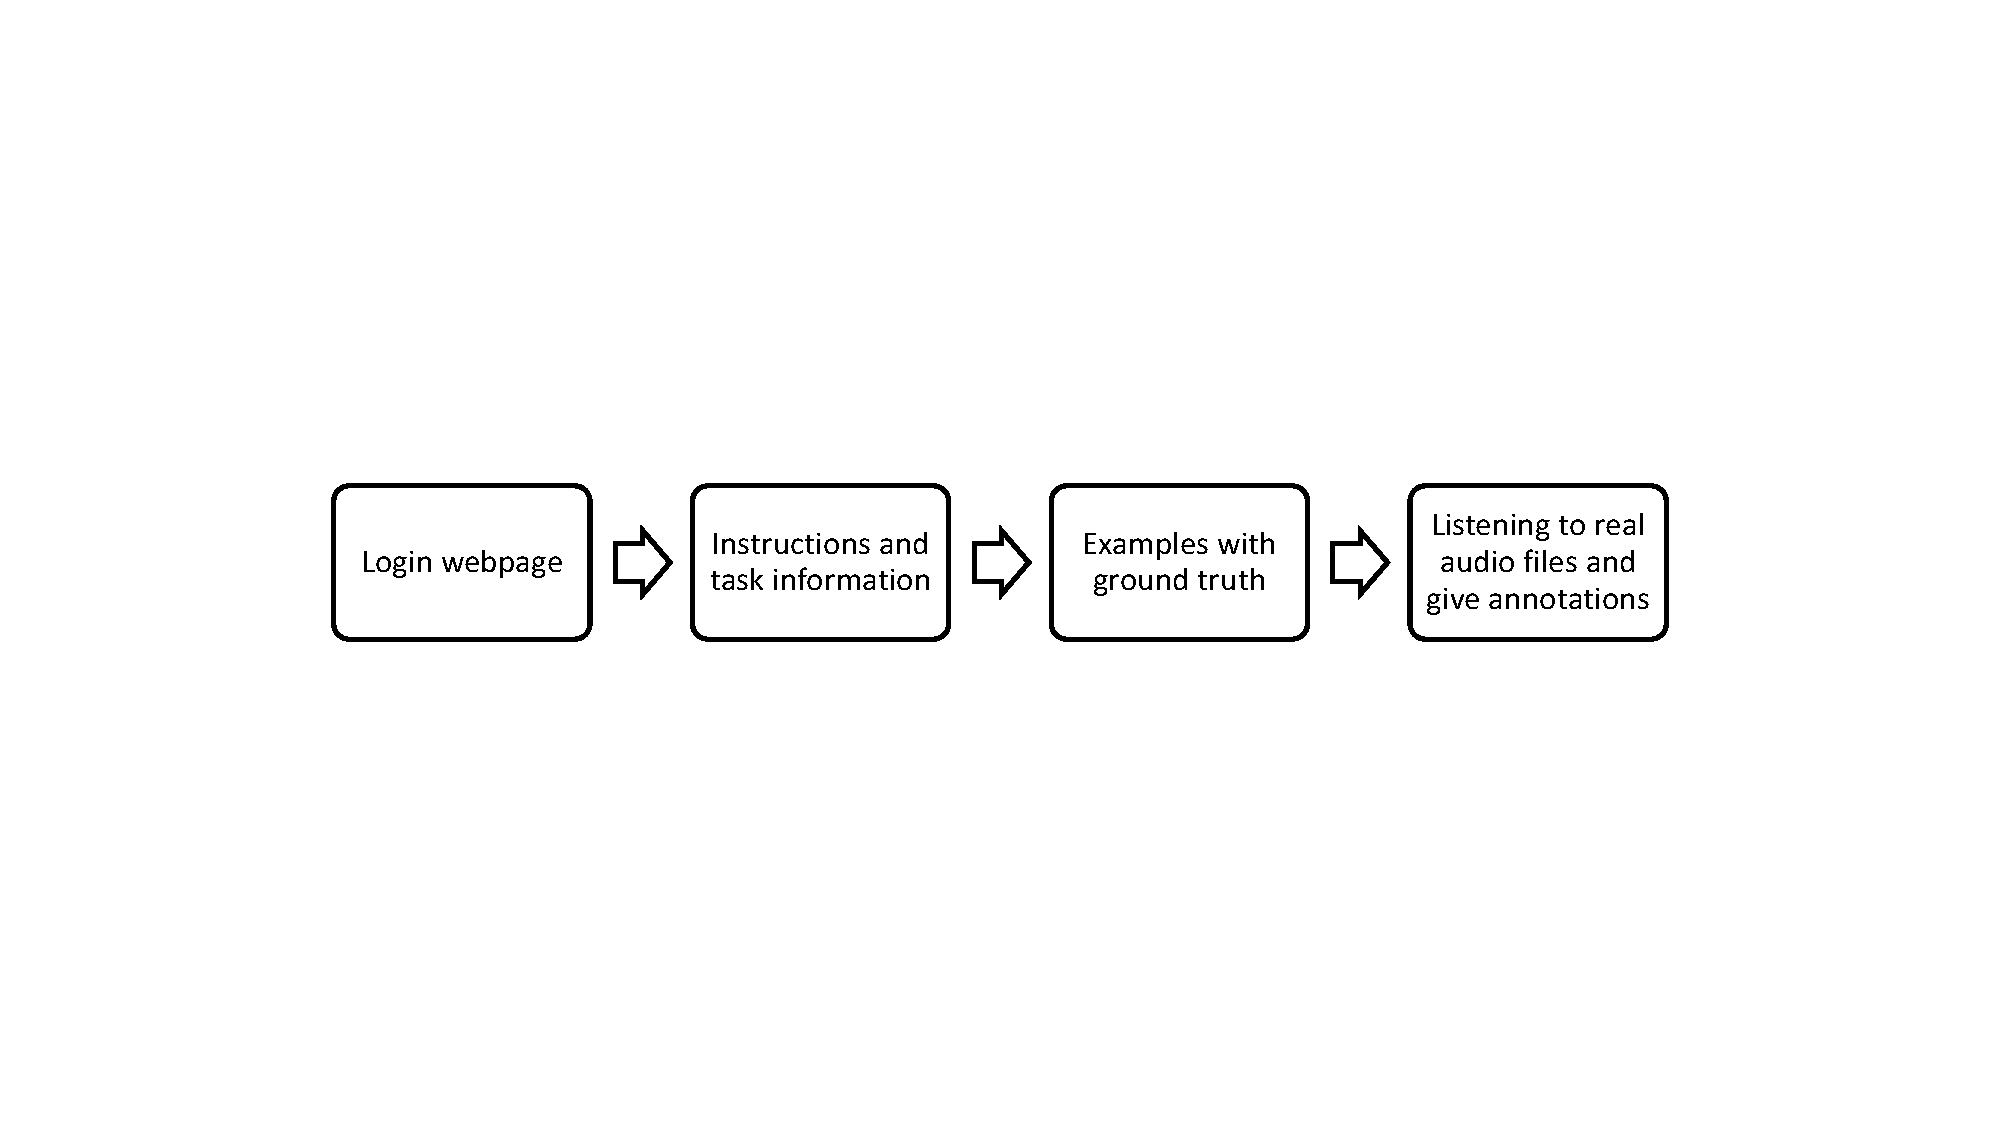
\includegraphics[width = 1.0\linewidth]{figures/amt_procedure.pdf}
\caption{The four steps of the annotation webpage.}
\label{fig:amt_procedure}
\end{figure}

\begin{enumerate}
\item The annotators will first see a webpage (as shown in figure \ref{fig:amt_login}), asking them to create a new user or login as a return user. The user ID will be used as identifier to locate their ratings.
\item After finishing step 1, a detailed task instruction and information will be shown to the annotators. The detail is in appendix \ref{sec:appendix1}. There is also a consent form (in appendix \ref{sec:appendix2}) for the annotators.
\item Then, four recordings, which are with no accent, mild accent, strong accent and very strong accent respectively, are presented to the annotators for them to get familarization with the 4-point rating scale, as shown in figure \ref{fig:amt_example}. The groundtruth labels are provided by experienced native American English speakers. This step also enables the annotators be familiar with the content of the recordings.
\item At last, annotators move to the real listening task, as shown in figure \ref{fig:amt_listen}. Each annotator first listens to the recording, then make a choice about the degree of perceived foreign accent and whether the annotator is confident in the response. All 150 speech recordings (including native English speech and accented speech) are randomly permuted in order. If the workers on AMT are asked to listen all of the utterances, the task would take more than 1 hour, and a lot of factors will impact the quality of the collected ratings, such as worker's fatigue \citep{rzeszotarski2013inserting}. To avoid this, all the utterances are segmented to retain only the first 10 seconds, resulting in 25 minutes listening time for each worker. Previous study \citep{munro1995foreign} has shown that the sentence length in the range of 7-13 seconds has little impact on the perceived accentedness. Considering the annotation time and a 2 minutes break, each worker needs to spend about 30-40 minutes for this task. Those annotators finish the task will be rewarded \$1.5.
\end{enumerate}


\begin{figure}[t]
\centering
\captionsetup{justification=centering}
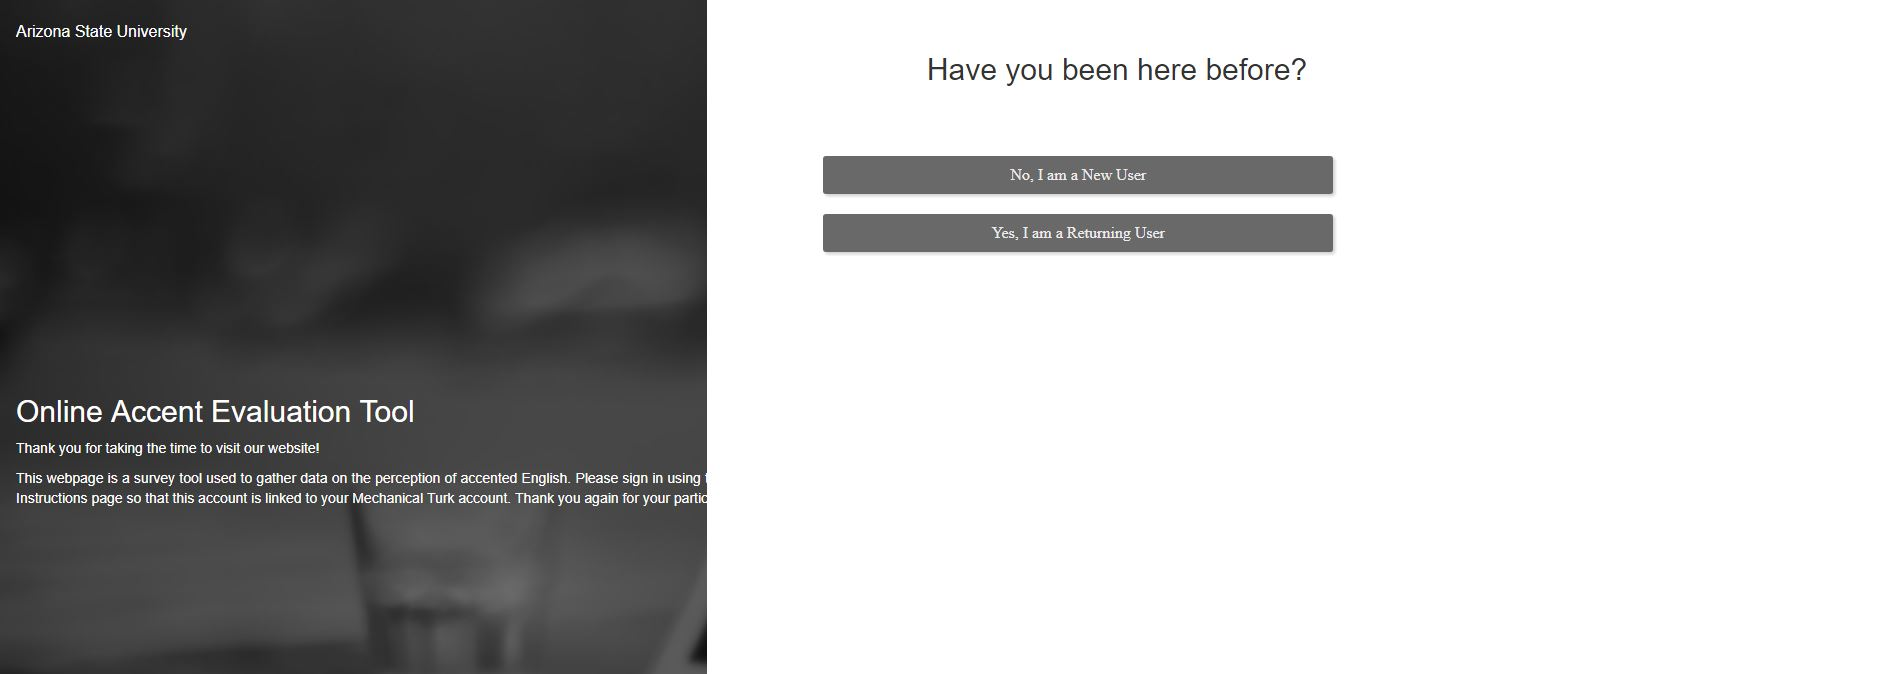
\includegraphics[width = 0.8\linewidth]{figures/webpage1.JPG}
\caption{Annotator's login page.}
\label{fig:amt_login}
\end{figure}

\begin{figure}[t]
\centering
\captionsetup{justification=centering}
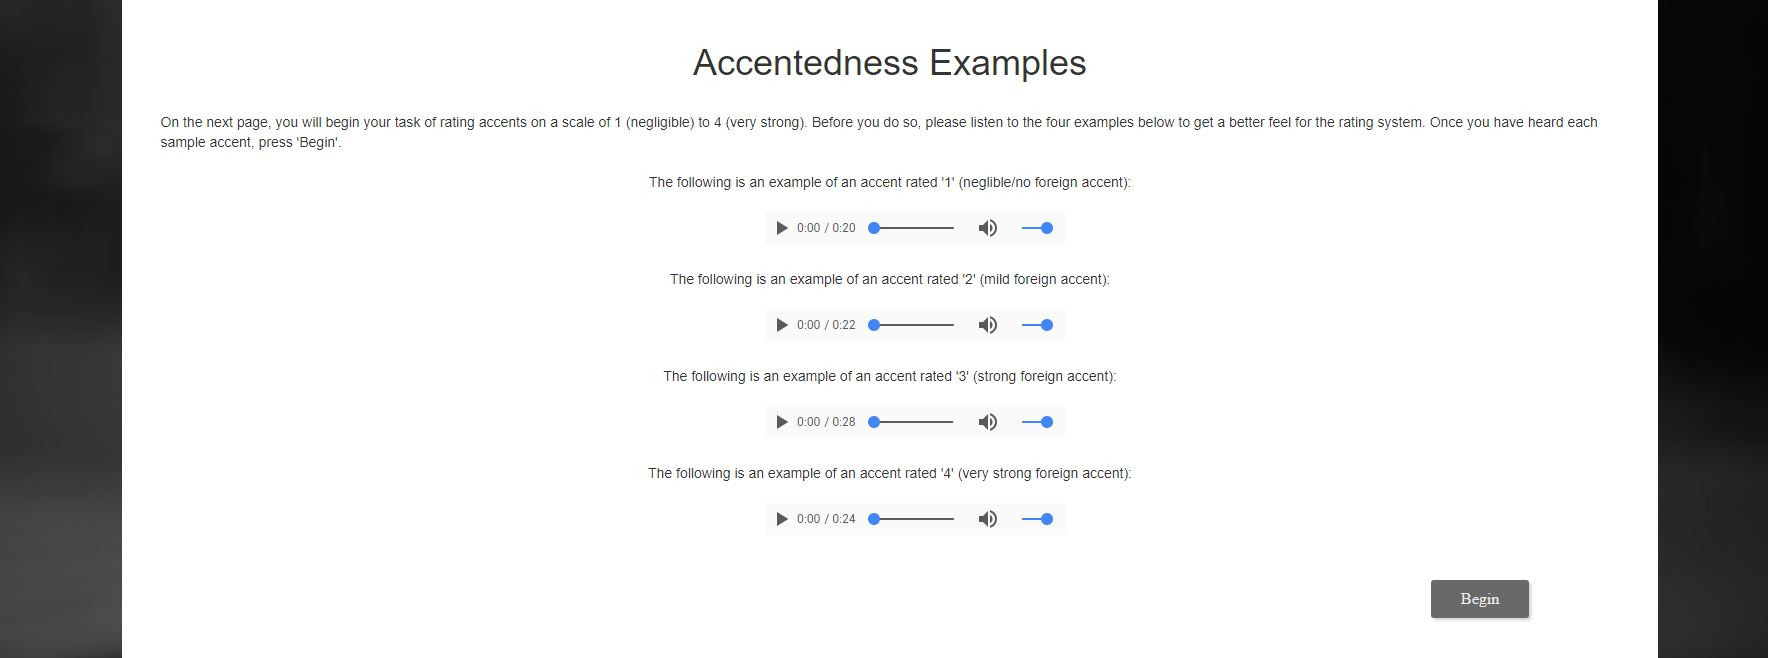
\includegraphics[width = 0.8\linewidth]{figures/webpage2.JPG}
\caption{Example accented speech recordings with groundtruth accentedness scores.}
\label{fig:amt_example}
\end{figure}

\begin{figure}[t]
\centering
\captionsetup{justification=centering}
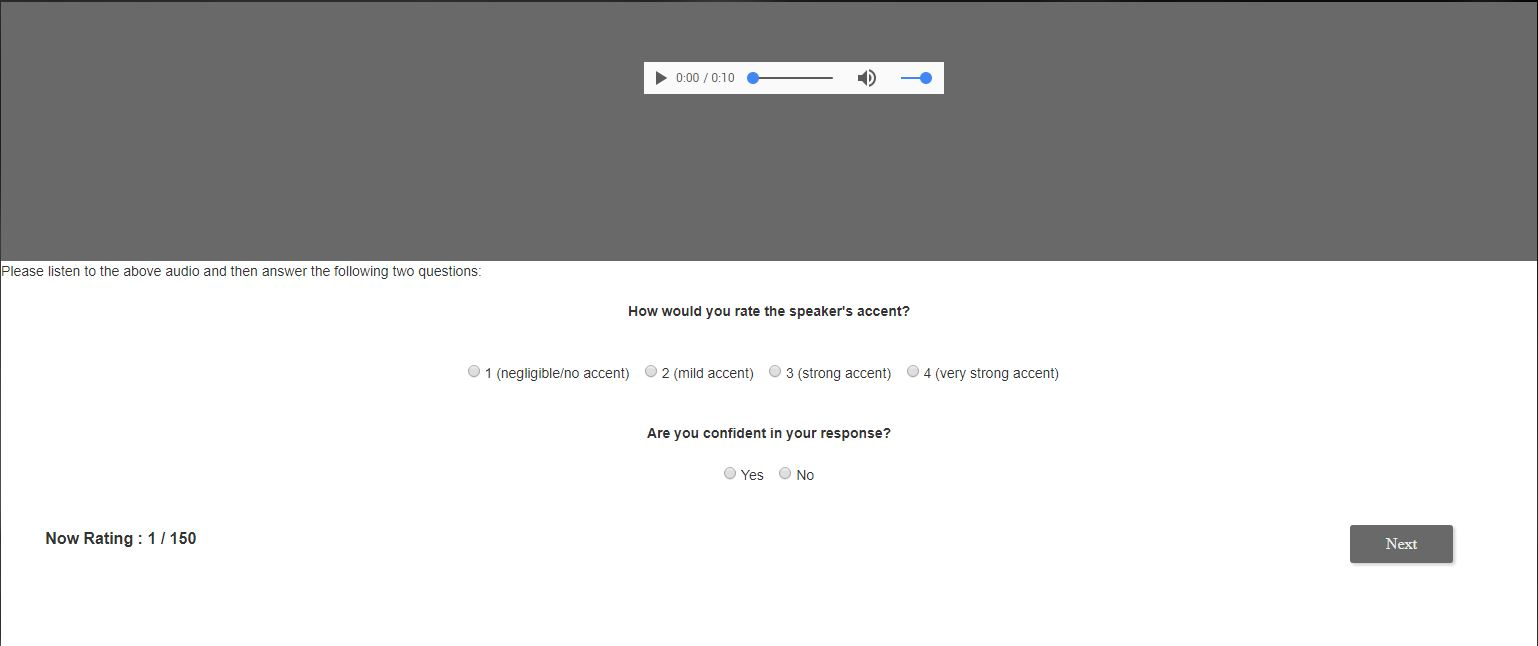
\includegraphics[width = 0.8\linewidth]{figures/webpage3.JPG}
\caption{How speech samples are presented to the annotators in listening task.}
\label{fig:amt_listen}
\end{figure}

Finally, 13 evaluators finished all the listening tasks. The average ratings of all 13 evaluators are taken as the final accentedness rating of each speaker; other studies have used the average of 10 AMT non-expert annotations in other natural language tasks \citep{snow2008cheap}. The pairwise average inter-rater correlation coefficients are shown in figure \ref{fig:pairwise_corr} for each rater, which is calculated by taking the average of the correlation coefficients of the current worker's ratings with other worker's ratings. The average inter-rater correlation coefficients (calculated as the average of all annotators' correlation with other annotators) is 0.73, which is higher enough to prove the consistency of the ratings from 13 evaluators. In figure \ref{fig0}, the histograms of the collected ratings across four different foreign languages are presented. It can be found that Mandarin speakers have the strongest accent while German speakers have the mildest accent. This is consistent with expectations considering the phonological similarity between German and English as opposed to other 3 languages. The low accentedness and lack of strongly-accented speakers in the German and French database also means that the variances of the accentedness ratings for these language are relatively low. This poses a challenge in the statistical modeling, which will be further examined in later chapters. In contrast, the average accentedness rating of native English speaker in the dataset is 1.07, which further validate the efectiveness of the annotation.

\begin{figure}[t]
\centering
\captionsetup{justification=centering}
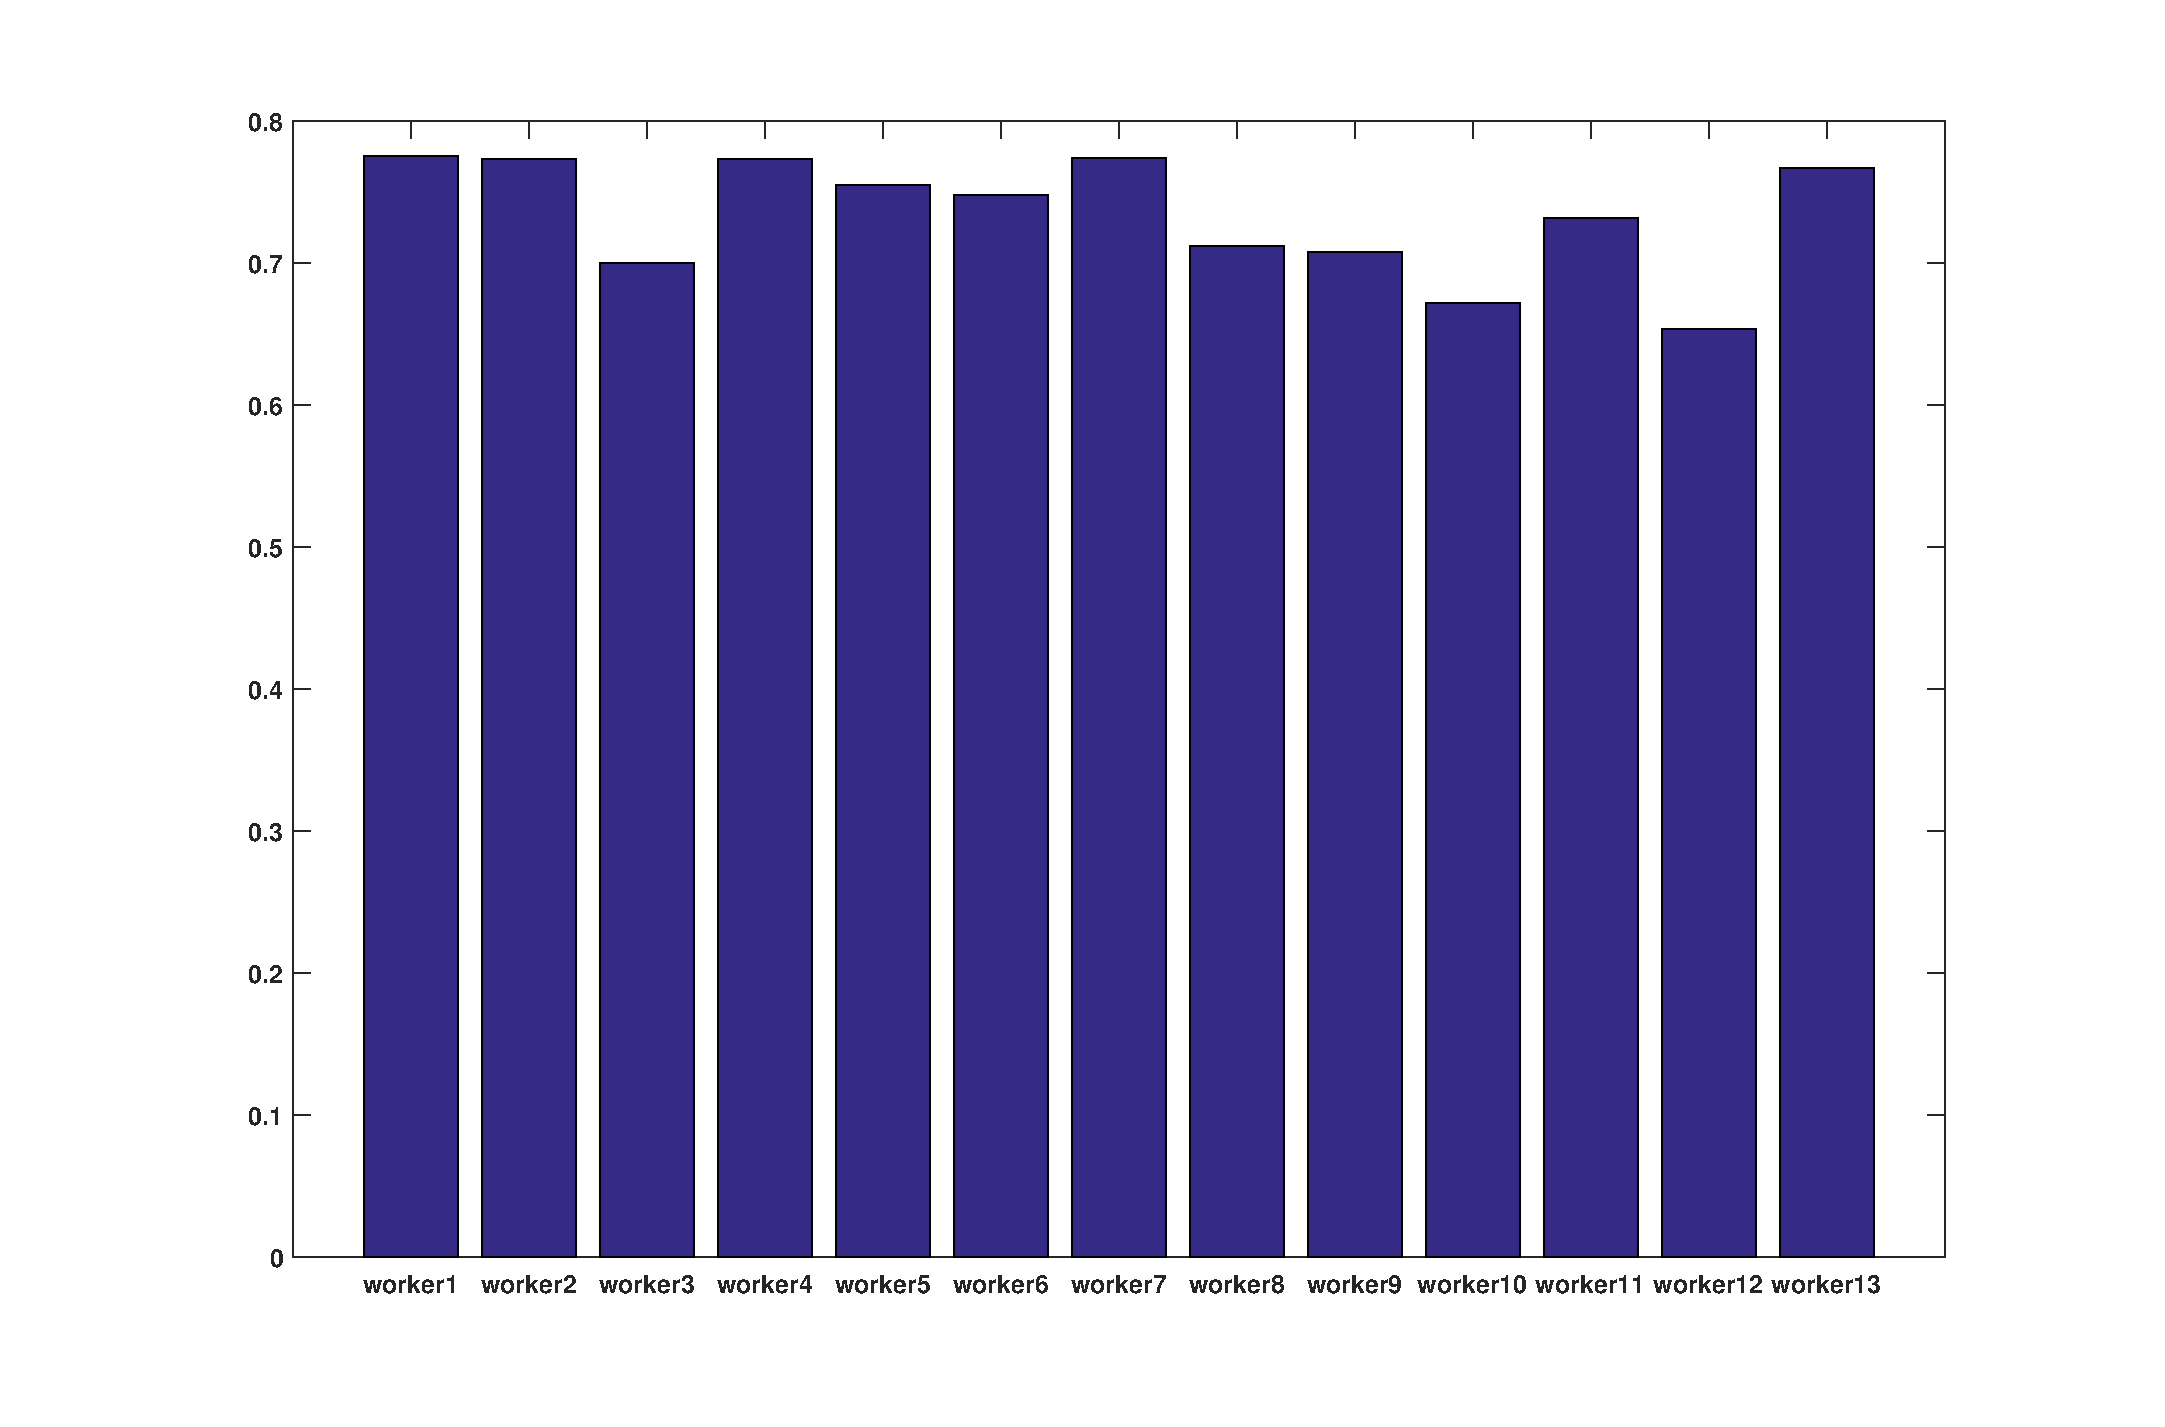
\includegraphics[width = 0.8\linewidth]{figures/mean_pairwise_correlation_without_work4.eps}
\caption{Pairwise average correlation coefficients of each worker.}
\label{fig:pairwise_corr}
\end{figure}

\begin{figure}[h]
        \begin{minipage}[t]{0.5\linewidth}
        \centering
            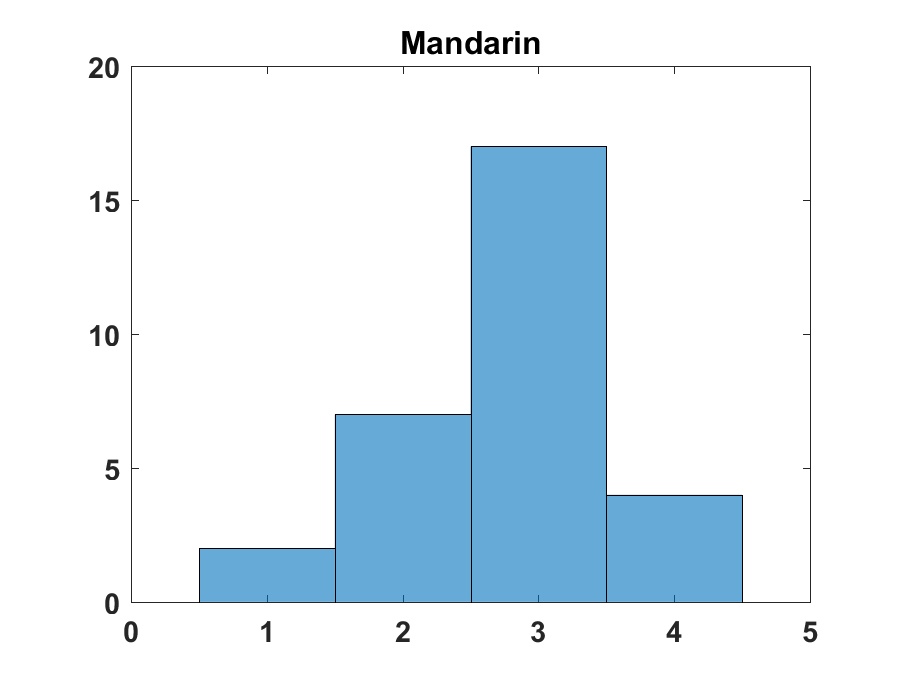
\includegraphics[width=3in]{figures/Mandarin_hist.eps}
        \end{minipage}%
        \begin{minipage}[t]{0.5\linewidth}
        \centering
            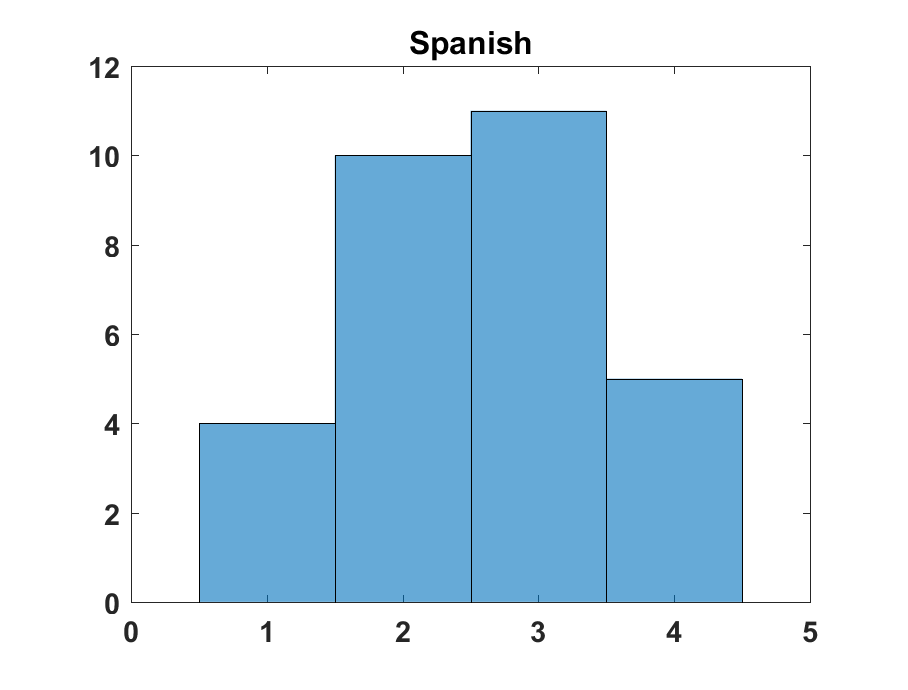
\includegraphics[width=3in]{figures/Spanish_hist.eps}
        \end{minipage}%
        \\
        \begin{minipage}[t]{0.5\linewidth}
        \centering
            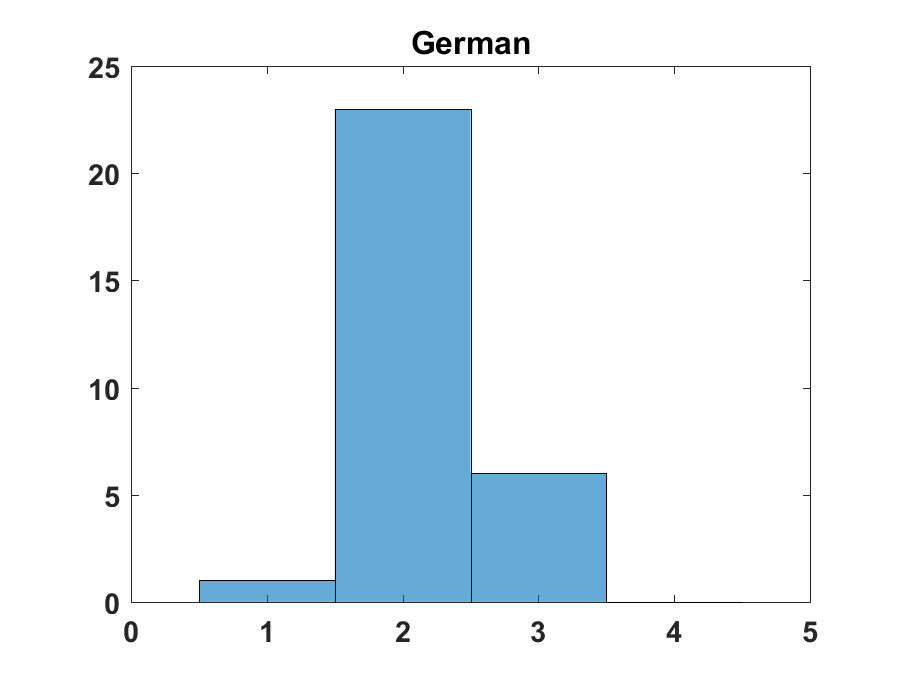
\includegraphics[width=3in]{figures/German_hist.eps}
        \end{minipage}%
        \begin{minipage}[t]{0.5\linewidth}
        \centering
            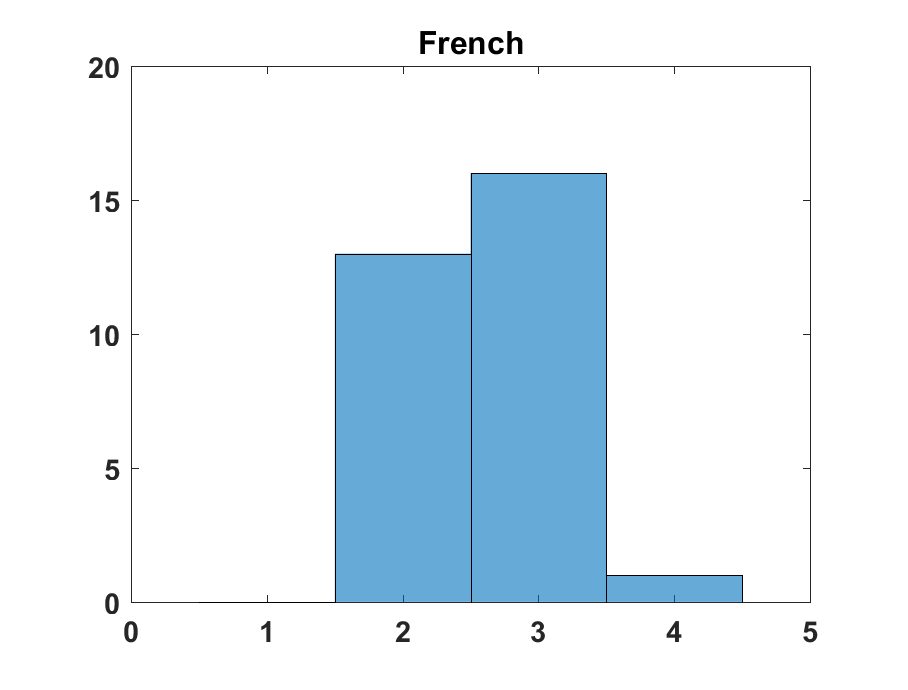
\includegraphics[width=3in]{figures/French_hist.eps}
        \end{minipage}%
        \caption{Histograms of accentedness scores of different L1s.}
        \centering
        \label{fig0}
     \end{figure}

\section{Acoustic analysis}

With the accentedness score for each speaker in the accented speech dataset collected, the next step is to extract measurements from the acoustic signal to represent the foreign accent. As mentioned in chapter \ref{introduction}, this study will analyze acoustic measurements in two subspaces: one is characterized by phonetic measurements and the other is characterized by prosodic measurements. Thus, the acoustic analysis here is also done in the two subspaces. Specifically, pronunciation scores of phonemes (including vowels and consonants) and syllables are calculated as representation of the phonetic subspace. The pronunciation scores are computed based on previous studies on phoneme-level goodness of pronunciation (GOP) \citep{witt2000phone}, which relies on an already-trained automatic speech recognition (ASR) system on native L2 speech. Prosodic measurements are calculated based on the studies by \cite{ramus1999correlates,grabe2002durational}. In this dissertation, more prosodic measurements are included as in \citep{lai2013applying}. Furthermore, the main contribution of this study is to investigate the relationship between L1 related acoustic measurements and accentedness scores. To calculate L1 related acoustic measurements, corpus of different L1s (German, French, Spanish and Mandarin in this study) are also needed. The remaining part of this section will first briefly review the basic concepts of an ASR system. Then, L1 corpus used in this study will be introduced. Finally, acoustic feature extraction scheme for both phonetic and prosodic information will be presented.

\subsection{A brief introduction to ASR}

\begin{figure}[t]
\centering
\captionsetup{justification=centering}
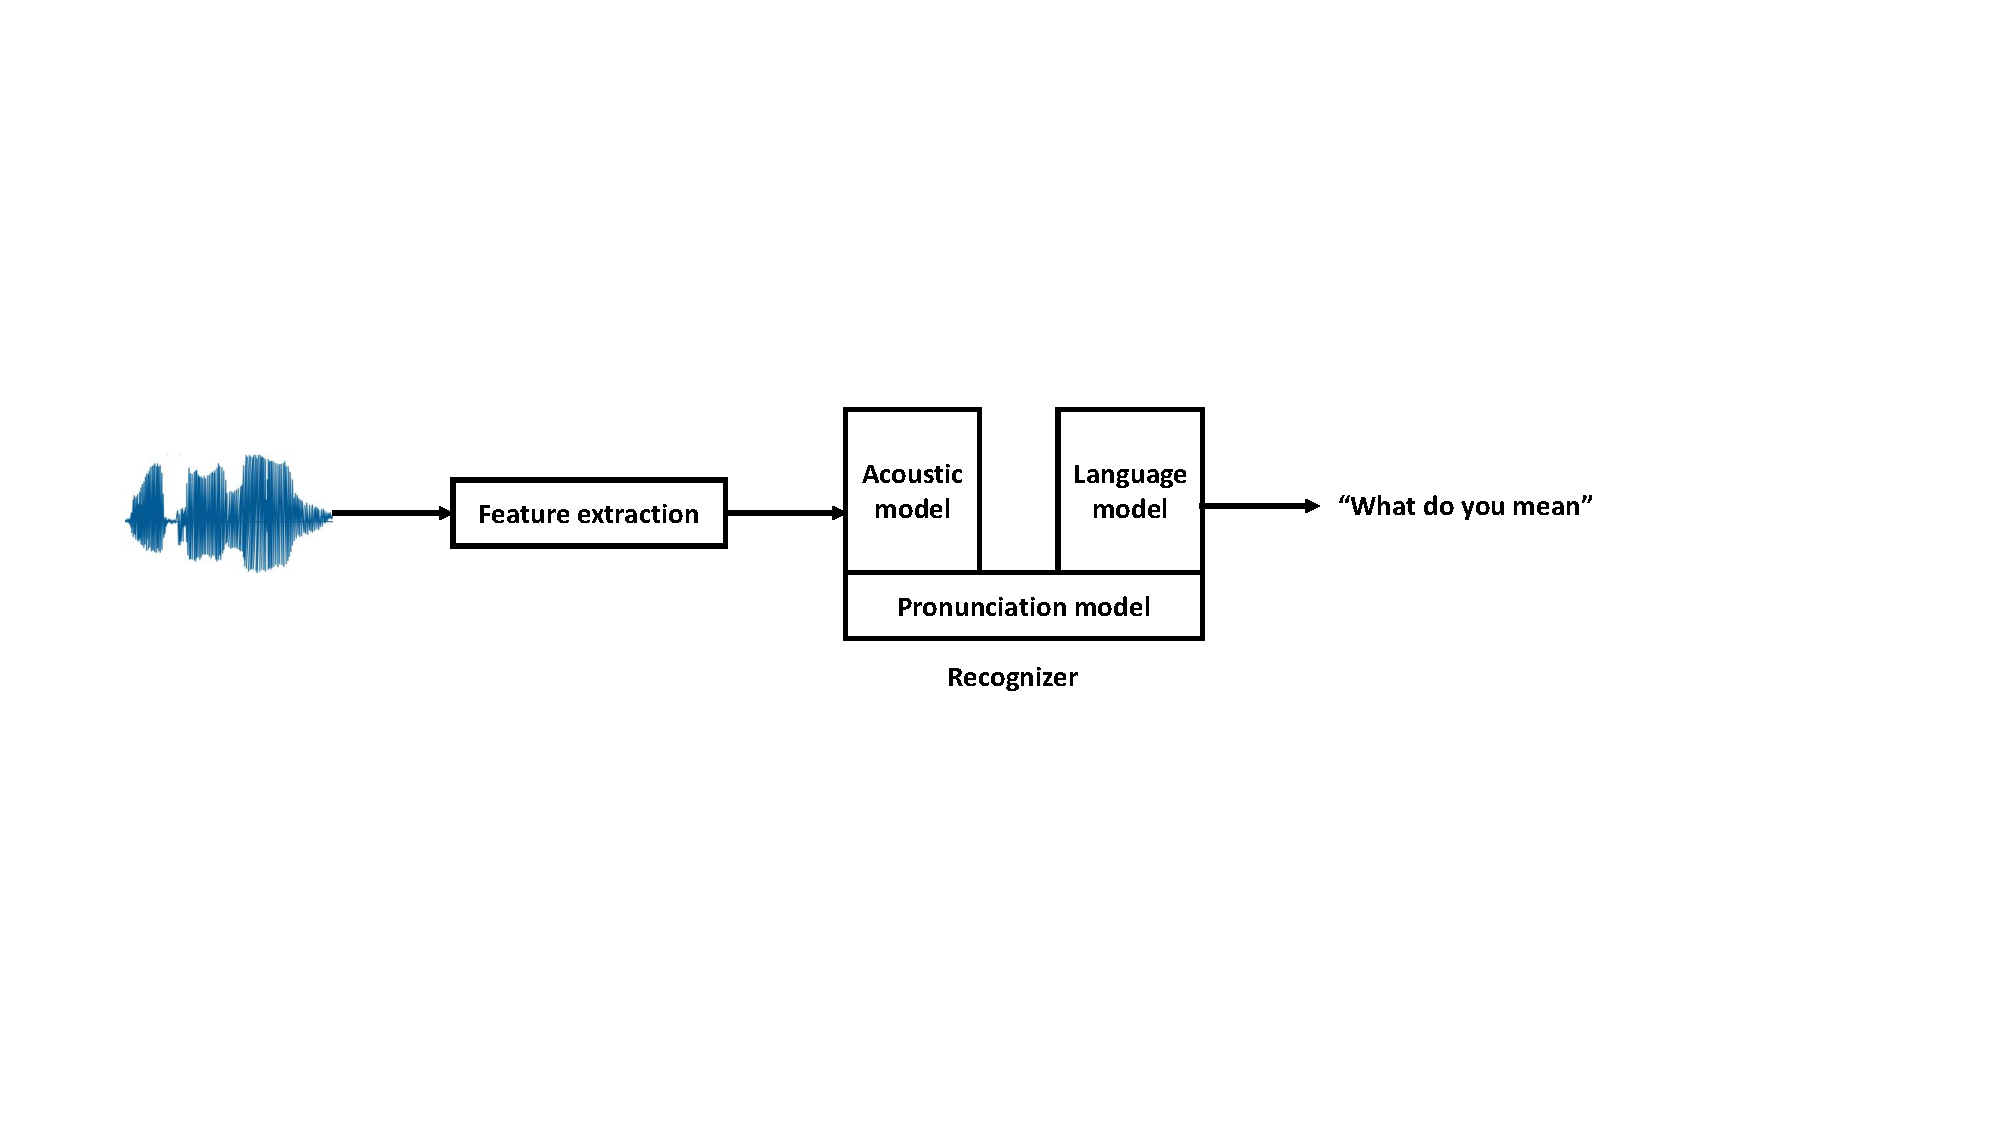
\includegraphics[width = 1.0\linewidth]{figures/ASR_diagram.pdf}
\caption{Diagram of a typical ASR system. The content of the speech signal is ``what do you mean''.}
\label{fig:asr_diagram}
\end{figure}

 Basically, ASR is trying to recognize the content, i.e. what the speaker is saying, in a speech signal. It requires knowledge from different fields, including psychoacoustics, signal processing, linguistics and machine learning\footnote{Recent developments on ASR mainly focus on the machine learning part.}. A simplified diagram of an ASR system is shown in figure \ref{fig:asr_diagram}. The input waveform is first analyzed within short windows (e.g. 25ms), which are also referred to as frames. Frame based analysis of speech signal is based on the assumption that spectral information is stationary in a short window. This process is done frame by frame. Then, a feature (usually based on Discrete Fourier Transformation, DFT) vector is calculated to represent the spectral information in each frame. The 1-dimensional time domain signal is then converted to a 2-dimensional time-frequency representation (DFT dimension $\times$ number of frames). Since phonemes can be discriminated based on spectral information in acoustic signal, this feature vector is believed to carry information of the identity of phonemes.

 \begin{figure}[t]
\centering
\captionsetup{justification=centering}
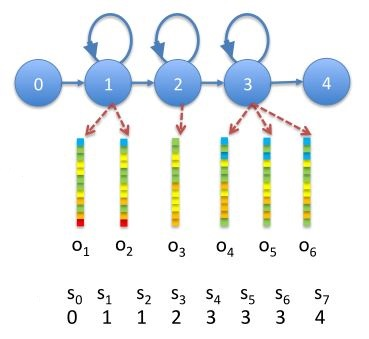
\includegraphics[width = 0.4\linewidth]{figures/HMM_state.JPG}
\caption{How an HMM aligns input feature vectors with the output state sequence.}
\label{fig:hmm_diagram}
\end{figure}

 Then, the feature vectors of a sentence are sent to a recognizer, which includes three parts: acoustic model, language model and pronunciation model. The acoustic model builds the relationship between feature representation and phonemes. A sequential machine learning model called Hidden Markov Model (HMM) is employed to learn the dynamic transition from one phoneme to another based on the observed feature vectors by aligning each frame with a state of an HMM model \citep{rabiner1989tutorial}. The reason to use HMM is that the number of frames is different from the number of phonemes in a sentence. There must be a way to correspond each frame to a sub-phoneme unit, which is called a state in an HMM. Each HMM models one phoneme, and the final acoustic model will have many HMMs. As the HMM shown in figure \ref{fig:hmm_diagram}, input feature vectors $o_1$ to $o_6$ are mapped to a state sequence $s_1$ to $s_6$, each of which corresponds to a state ID in $\{1,2,3\}$. At each frame, it either moves to the next state or stay at the current state. State 0 and 4 are the entrance and exit states of the HMM, which allows transition from a previous phoneme and exit from the current phoneme. Most of the time, a triphone(for example [k-ae+t], [k] is to the left of [ae] and [t] is to the right) instead of a single phone([ae]) is used as the basic modeling unit of an HMM, for the reason that triphone can better model the coarticulation among neighboring phonemes and improve model capability. The possibility a feature vector in one frame is generated by a specific HMM state is modeled with a Gaussian Mixture Model (GMM) or Deep Neural Network (DNN). The possibility a state is transited from another state is decided by an HMM. In summarization, the acoustic model converts a sequence of feature vectors to a sequence of HMM states (with GMM-HMM or GMM-DNN models), and then to phoneme sequence according to the mapping from HMM states to phonemes.

 The language model is to convert phoneme sequences output by acoustic model to feasible word sequences, which complies with human usage of words. The pronunciation model involves in this process: it gives the phoneme sequence of each single word in a language. In a nutshell, the pronunciation model is just the lexicon(or dictionary) of a language in most of the time. Pronunciation model will also be used to convert word sequences in transcriptions to phoneme sequences during training stage of the acoustic mode. There is another term commonly seen in ASR field: forced-alignment. It refers to the process to find the start and end time of a phoneme, word or even sentence in a speech signal given the transcription. This can be achieved using acoustic model and pronunciation model. A lot of studies in computational linguistics use forced-alignment to avoid locating phonemes and words in a speech signal by hand. Practically, Kaldi toolkit \citep{povey2011kaldi} is the most commonly used software to build an ASR system, and it has been well accepted by both academia and industry.

\subsection{Native speech corpus}
In this study, both the L2 and L1s acoustic models and pronunciation models are needed to extract pronunciation score based phonetic features. To build the L2 acoustic model (English for this study), the LibriSpeech corpus \citep{panayotov2015librispeech} with 960 hours of native English speech recordings was used, and the corresponding training scripts\footnote{https://github.com/kaldi-asr/kaldi/tree/master/egs/librispeech/s5} in the Kaldi toolkit. The final acoustic model is a triphone model trained with GMM-HMM on 960 hours of speech data. The feature input is a 39-dimensional second order Mel-Frequency Cepstral Coefficient (MFCC) with utterance-level cepstral mean variance normalization and linear discriminant analysis transformation.

For Mandarin, the publicly accessible AIShell Mandarin Speech corpus (approximately 150 hours training data) \citep{bu2017aishell} and the corresponding Kaldi scripts\footnote{https://github.com/kaldi-asr/kaldi/tree/master/egs/aishell/s5} are used. A pronunciation dictionary is included in the dataset. For the remaining three languages (Spanish, French and German), there are no well organized publicly available data. This study uses data from the Voxforge project, and downloads the speech corpora for French ($\approx$ 30 hours), German ($\approx$ 50 hours) and Spanish ($\approx$ 50 hours). Kaldi scripts\footnote{https://github.com/kaldi-asr/kaldi/tree/master/egs/voxforge/s5} for the Voxforge English dataset are adapted to train the acoustic models of the three foreign languages. The dictionary for these three languages are from the CMU Sphinx system (Download available\footnote{https://sourceforge.net/projects/cmusphinx/files/Acoustic\%20 \\ \hspace*{4mm} and\%20Language\%20Models/}). Compared to English and Mandarin acoustic models, the quality of the German, French and Spanish acoustic models trained on Voxforge dataset are not that good (due to varying vocabulary sizes, different number of speakers across languages; some recordings are with background noise; pronunciation model is not designed for the datasets). Feature types and structures of acoustic models for the four languages are the same as those used in the English acoustic model.

\subsection{Pronunciation score based phonetic feature extraction}
\label{sec:segmental}

\subsubsection{Features based on the L2 acoustic model}
\label{sec:L2_measure}

The trained L2 acoustic model can be regarded as the phonetic patterns of native L2 speakers, and it is natural to measure how good non-native L2 speakers' pronunciation is with the native L2 phonetic patterns. Motivated by the work by \cite{witt2000phone}, the goodness of pronunciation for each phoneme is calculated in the accented speech. To do this, the accented speech is first force-aligned at the phoneme-level using the L2 acoustic model to provide the start and end frame indices of each phoneme. The pronunciation score ($PS_{\mathrm{L2}}$) of the target phoneme $p$ after alignment is defined as
\begin{equation}
\label{gop}
\begin{aligned}
PS_{\mathrm{L2}}(p) &= \log(P(p|\mathbf{O}^{p}))/\left | \mathbf{O}^{p} \right | \\
      &= \log \left [ \frac{P(\mathbf{O}^{p}|p)P(p)}{\sum_{q\in \mathit{Q}} P(\mathbf{O}^{q}|q)P(q)} \right ] /\left | \mathbf{O}^{p} \right |,
\end{aligned}
\end{equation}
where $\mathbf{O}^{p}$ is the feature matrix of phoneme $p$, $\left |\mathbf{O}^{p}\right |$ is the number of frames of phoneme $p$ after alignment, and $\mathit{Q}$ is the set of all phonemes. If we assume equal priors for all phonemes, we approximate the denominator in Eq. \ref{gop} with max operator,

\begin{equation}
\label{gop2}
PS_{\mathrm{L2}}(p) = \log \left [ \frac{P(\mathbf{O}^{p}|p)}{\max_{q\in \mathit{Q}} P(\mathbf{O}^{q}|q)} \right ] /\left | \mathbf{O}^{p} \right |.
\end{equation}

The conditional likelihood of each phoneme (given the speech frames of the corresponding aligned segment) can be calculated by decoding the sequence of speech features using the L2 acoustic model. It is clear that if the most likely phoneme returned by the acoustic model is the same as the target phoneme $p$, then $PS_{\mathrm{L2}}(p)=0$; otherwise, this value will be negative. The interpretation is that the closer $PS_{\mathrm{L2}}(p)$ is to zero, the closer the pronunciation of phoneme $p$ is to that of native speakers.

\subsubsection{L1 acoustic model based measurements}
\label{sec:L1_measure}

Similarly, the trained L1s acoustic models can be regarded as the phonetic patterns of the L1s of accented speakers. These phonetic patterns can decide how much the pronunciation of L2 is influenced by accented speakers' L1s. In contrast to the $PS_{\mathrm{L2}}$ score, there is no transcript to measure the pronunciation of the phonemes in L1. We define a new way to calculate the pronunciation score with the L1 acoustic model which quantifies how close the pronunciation of a phoneme in L2 is to a specific phoneme in L1. The forced-alignment calculated with the L2 acoustic model is used here. The speech frames are first decoded with the L1 acoustic model and find the state path with the highest likelihood. In the path, the corresponding phonemes of each HMM state are recorded and the phoneme with the highest occurrence is considered as the most likely L1 phoneme for a given speech segment. Then, the pronunciation score is calculated as

\begin{equation}
\label{l1gop}
PS_{\mathrm{L1}}(p) = \left [ \sum_{t \in T_p} \log \frac{ \sum_{s \in S_p}P(o_t|s)}  { \sum_{s \in S}P(o_t|s)} \right ] /\left | T_p \right |,
\end{equation}
where $o_t$ is the feature vector for frame $t$ and $p$ is the phoneme with the highest occurrences in the best decoding path of the current segment. $T_p$ is the set of frames where each frame corresponds to an HMM state of phoneme $p$. $S_p$ is the set of HMM states that belong to phoneme $p$ and $S$ is the set of all HMM states. $PS_{\mathrm{L1}}(p)$ essentially quantifies the confidence of the L1 acoustic model that phoneme $p$ was produced for a speech segment. With equation \ref{l1gop}, a pronunciation score based on the L1 acoustic model can be calculated for each phoneme segment in the original alignment. The implementations of both feature sets are available on Github\footnote{https://github.com/tbright17/kaldi-dnn-ali-gop}.

\subsubsection{Sentence-level integration}

Previous introduced feature extraction methods will output both $PS_{\mathrm{L2}}$ and $PS_{\mathrm{L1}}$ on phoneme level. However, accented speech of each speaker is a sentence. Thus, a sentence-level integration method is proposed to convert phoneme-level pronunciation scores to a sentence-level feature vector. Specifically, after phoneme-level features $PS_{\mathrm{L2}}(p)$ and $PS_{\mathrm{L1}}(p)$, are extracted, a sentence-level feature extraction scheme was used to convert phoneme-level measurements to a feature vector with a fixed dimension for each utterance. The pronunciation features for vowels, consonants and syllables are first grouped together, and four statistics for each of these three phonetic categories are then calculated: for both $PS_{\mathrm{L2}}(p)$ and $PS_{\mathrm{L1}}(p)$, the minimum, mean, standard deviation and mean-normalized standard deviation (standard deviation divided by mean) of phoneme-level pronunciation scores of vowels, consonants and syllables in each utterance are calculated (implementation available\footnote{https://github.com/tbright17/accent-feat}). This results in a total of 12 utterance-level features, and a total of 24 utterance-level features combining both pronunciation information from L1 and L2 acoustic models.

\subsection{Prosodic feature extraction}
\label{sec:supraseg}

To represent speech prosody, durational rhythmic measurements of phonemes and syllables are adopted as the studies by \cite{ramus1999correlates,grabe2002durational}. Specifically, an extended speech rhythmic feature set proposed in \citep{lai2013applying} are employed in this study. First, the same forced-alignment results achieved in previous section is reused here to get the start and end time of each phoneme. Then, the following measurements are calculated:
\begin{enumerate}
\item Mean, standard deviation and mean-normalizd standard deviation (standard deviation divided by mean) of durations of vowels, consonants and syllables.
\item Duration proportion of vowels, consonants and syllables, calculated as the total length of vowels, consonants and syllables divided by the length of the sentence (with starting and ending silence removed).
\item Raw Pairwise Variability Index (rPVI) of durations of vowels, consonants and syllables, calculated as:
    \begin{equation}
    \label{eq:rPIV}
    rPVI= \sum_{k=1}^{m-1} |d_k-d_{k+1}|/(m-1),
    \end{equation}
    where $d_k$ is the duration of $k$th phoneme or syllable and $m$ is the total number of phonemes or syllables in a sentence.
\item Normalized Pairwise Variability Index (nPVI) of durations of vowels, consonants and syllables, calculated as:
    \begin{equation}
    \label{eq:nPIV}
    nPVI= \sum_{k=1}^{m-1} |\frac{d_k-d_{k+1}}{(d_k + d_{k+1})/2}|/(m-1),
    \end{equation}
    where the notations are the same as in equation \ref{eq:rPIV}.
\end{enumerate}

Finally, a 18-dimensional feature vector can be extracted from each speech signal. In this study, this rhythmic feature extraction scheme is applied to both L1 speech, L2 speech and accented speech to do contrastive analysis between accented speech and L1, and between L2 speech and accented speech. For the four foreign languages, 1000 sentences with more than 40 phonemes in each are randomly selected from the corresponding native speech corpus. In order to achieve better forced-alignment, another forced-alignment tool \citep{mcauliffe2017montreal} is employed to align phoneme sequences with speech recordings because it comes with well-trained foreign language acoustic models (However, because of lack of information, it can not be used to do the computation in section \ref{sec:L1_measure}). For native English speech, those measurements are directly calculated on the 30 native American English sentences from SAA using the native English acoustic model trained on Librispeech dataset. The average of rhythmic features of each language (four L1s and English) will be used as the speech prosodic patterns of those languages.

\section{Procedure}

 \begin{figure}[t]
\centering
\captionsetup{justification=centering}
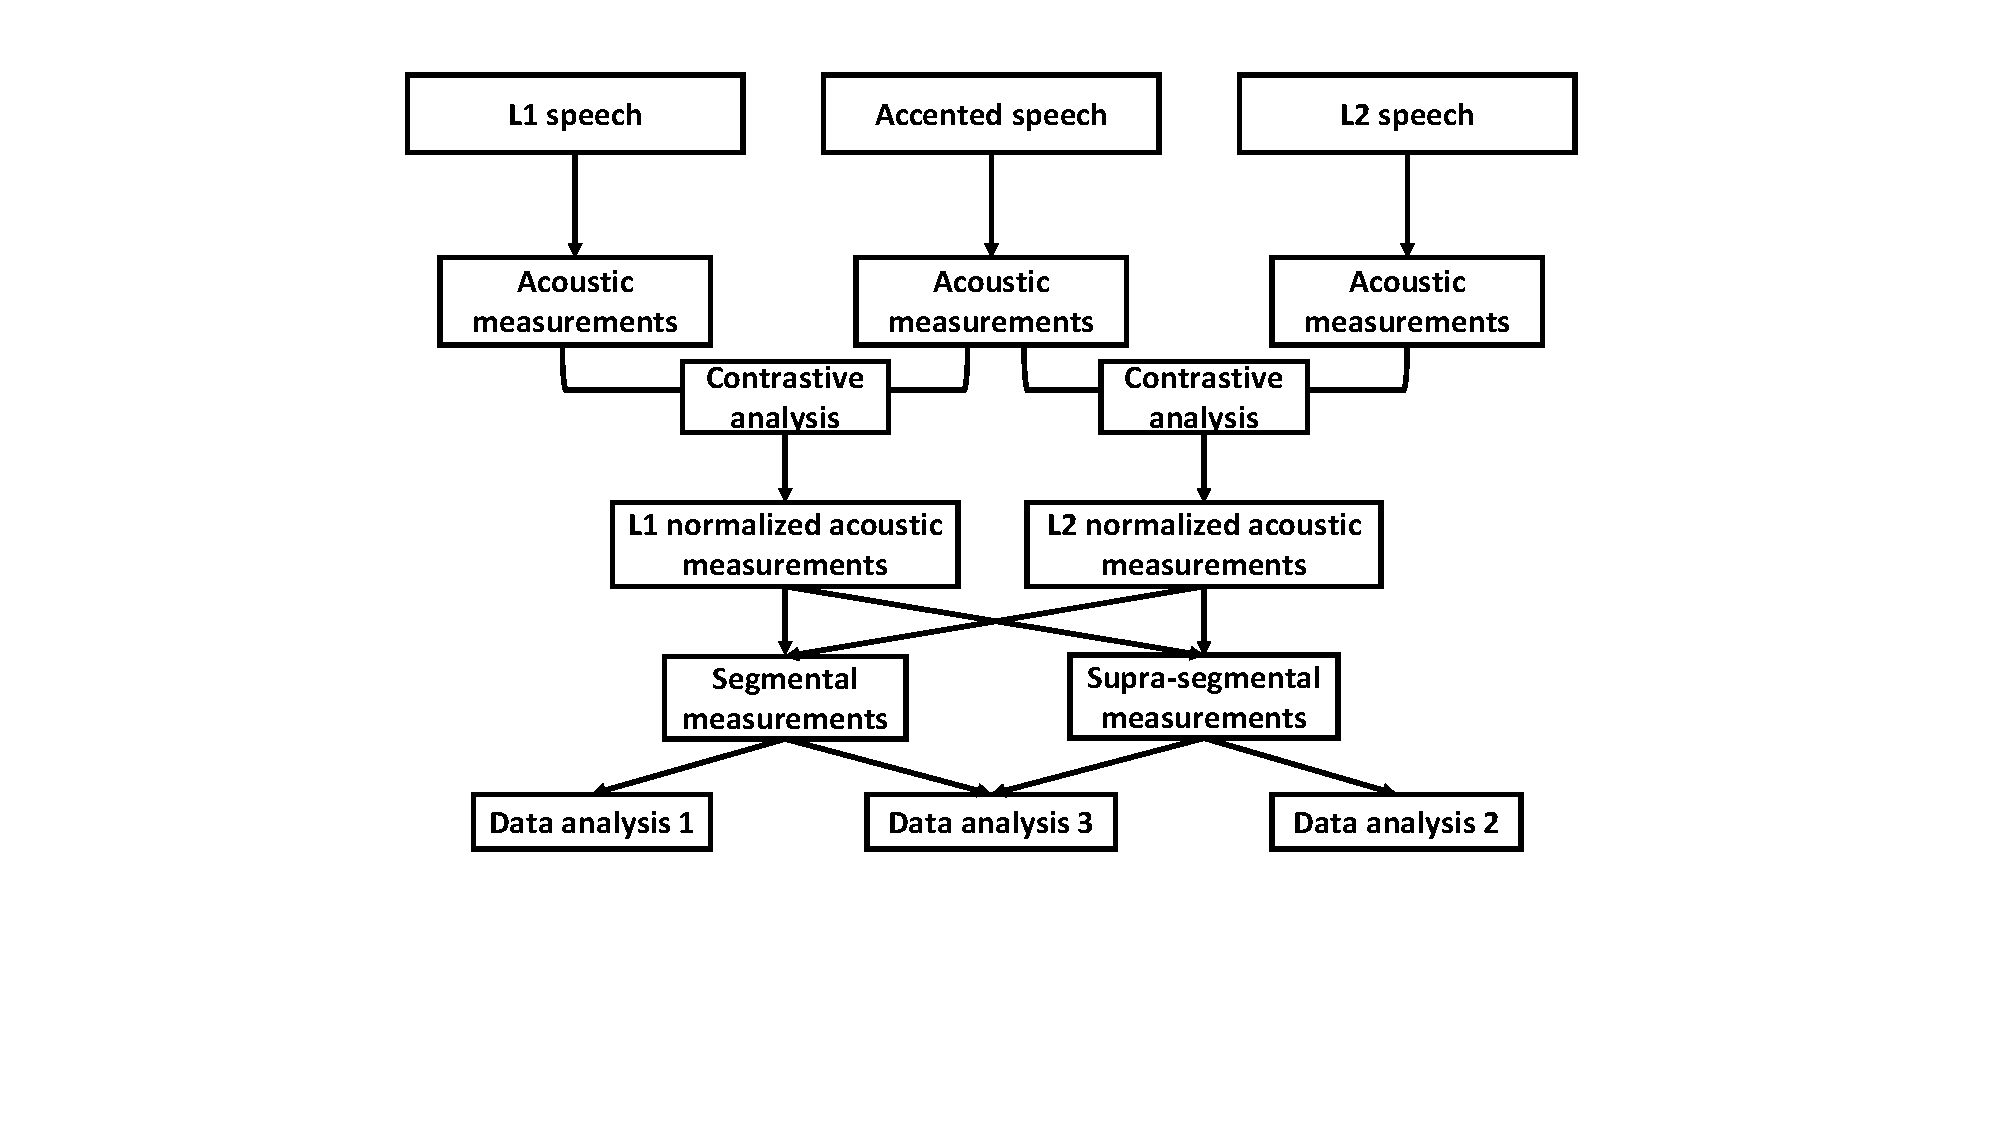
\includegraphics[width = 0.8\linewidth]{figures/method_diagram.pdf}
\caption{Diagram of the methodology used in this study.}
\label{fig:method_diagram}
\end{figure}

The diagram of the methodology used in this study is shown in figure \ref{fig:method_diagram}. After extracting acoustic measurements from native L1 speech, accented speech and native L2 speech, differential analysis, the goal of which is to quantify the difference between two sets of features, is applied to the L1-accented pair and L2-accented pair. Then, two sets of features can be obtained: the L2 normalized acoustic measurements represent how close the phonological properties in accented speech is to native L2 speech; the L1 normalized acoustic measurements represent how close the phonological properties in accented speech is to native L1 speech. The segmental feature extraction scheme in section \ref{sec:segmental} directly output the L1 and L2 normalized acoustic measurements. This is because the input to that scheme in this case is accented speech and L1 or L2 phonetic patterns (defined by L1 or L2 acoustic models), and the output can represent the difference between accented speech and L1/L2 phonetic patterns. In contrast, differential analysis needs to be done for the suprasegmental feature extraction method in section \ref{sec:supraseg}. The L2 and L1 normalized feature sets can be further categorized into segmental measurements and suprasegmental measurements. The first data analysis, which will be introduced in chapter \ref{l1_seg}, will investigate the effect of L1 phonetic patterns on the perception accented speech.  The second data analysis, which will be introduced in chapter \ref{l1_supraseg}, will investigate the effect of L1 prosodic properties on the perception of accented speech. The third data analysis, which will be introduced in chapter \ref{both_l1_l2}, will investigate the effect of L1 phonetic and prosodic patterns on the perception of accented speech, and propose a new computational model to do automatic accentedness evaluation. The data analysis methods used in this study are mainly correlation analysis, which examines how the acoustic measurements and accentedness score are correlated, and multiple regression analysis, which examines how well the combination of multiple acoustic measurements can predict the accentedness score. The whole data analysis procedure involves feature preprocessing, feature selection and mode regularization, which will be introduced in detail in later chapters.

\chapter{L1's effect on phonetic properties of accented speech}
\label{l1_seg}

\section{Introduction}

This section will investigate the statistical relationship between the phonetic acoustic measurements extracted from accented American English speech (independent variables) and the perceived accetendenss score provided by native American English speakers (dependent variables). Two sets of features will be used as independent variables: one is the pronunciation score based features extracted only using L2 acoustic model and the other one is the pronunciation score based features extracted using both L1 and L2 acoustic model. This corresponds to the data analysis 1 in figure \ref{fig:method_diagram} using only L2 normalized segmental acoustic measurements and the combination of  both L1 and L2 normalized segmental acoustic measurements. First, correlational relationship between independent variables and dependent variables. Second, multiple regression analysis will be employed to analyze how well each set of features can predict the accentedness score. Results and discussion are in the final part.

\section{Methods}


For each foreign language, the correlation analysis will be done between each dimension of the feature vector and the accentedness scores ( average of all 13 annotators). The correlation analysis is done L1 independently in hope that some L1 specific information will be revealed. The Spearman correlation coefficients and the corresponding p-value for testing non-correlation will be calculated in this part. Higher correlation coefficients means better correlation and lower p-value means correlation is more significant.

\begin{figure}[t]
        \begin{minipage}[t]{1\linewidth}
        \centering
            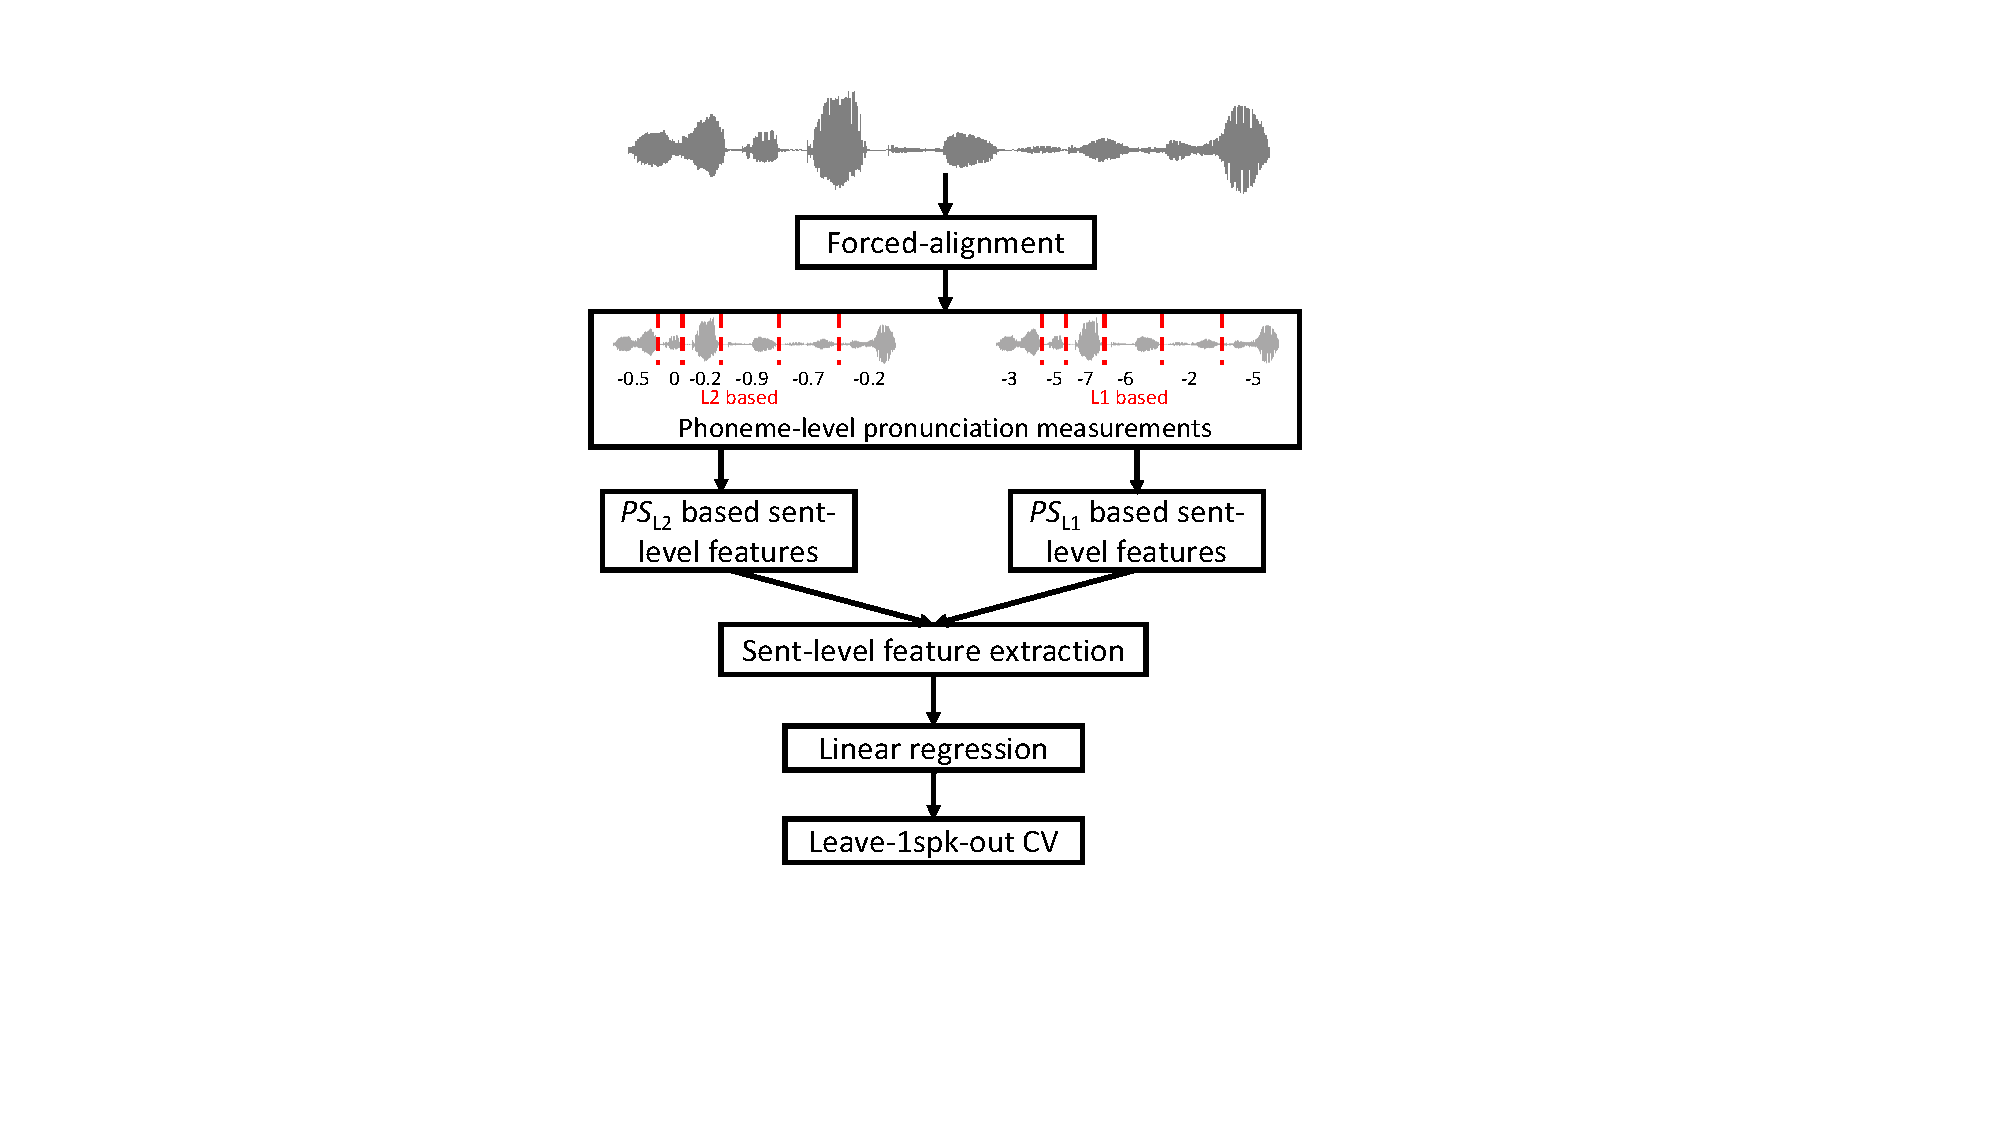
\includegraphics[width=3.0in]{figures/L1_seg_diagram.pdf}
        \end{minipage}%
        \caption{Diagram of the procedure for multiple regression analysis between pronunciation based acoustic measurements and accentedness score.}
        \centering
        \label{fig:l1_seg_diagram}
     \end{figure}

The whole procedure of multiple regression analysis is shown in figure \ref{fig:l1_seg_diagram}. The upper part of the figure shows the feature extraction scheme in section \ref{sec:segmental} and will not be described here. Each speaker had a 12-dimensional feature vector quantifying how close their pronunciation is to L2 and another 12-dimensional feature vector quantifying how close their pronunciation is to their L1.. After extracting utterance-level features for all speakers, each speaker has a feature vector and a corresponding accentedness score (in the range of 1 to 4). For speakers that belong to the same L1 category, a linear regression model with an L2 norm regularizer (or ridge regression) is built with data from 29 speakers used to train the model and the remaining speaker used to evaluate the model. The feature vectors were mean and variance normalized first. Feature selection based on univariate linear regression test \citep{saeys2007review} was also used to select the most predictable features. Basically, the feature selector calculates a score (based on the correlation coefficients between independent variables and dependent variables) for each independent variables given labels in training set and select the independent variables with highest scores. The scikit-learn toolkit was used to implement feature normalization, feature selection and ridge regression \citep{scikit-learn}. To generate the accentedness prediction for all speakers, evaluation using leave-one-speaker-out CV was performed; this means that a feature selector and a ridge regression model is trained on all combinations of 29 speakers out of 30 speakers and tested on the 1 remaining. For different input features (12-dimensional utterance-level features or 24-dimensional utterance-level features), the hyperparameters were tuned to achieve the best performance.

As mentioned in section \ref{sec:data_collection}, the accentedness label distributions for German and French speakers do not span the 1-4 rating scale uniformly. The initial result revealed that the model performance on German and French speakers was comparatively lower (but there was still improvement by adding the feature vector extracted using L1 acoustic model). In an attempt to train our model with more uniformly distributed labels, the German speakers were randomly downsampled from 30 to 18 and French speakers from 30 to 22 in an attempt to uniformly sample the labels. For other two languages, there are still 30 speakers in the results. The Pearson correlation coefficient (PCC, higher better) and the mean absolute error (MAE, lower better) are used to measure the relationship between model prediction and human scores.

\section{Results}

\subsection{Results of correlation analysis}

\begin{table}[]
\centering
\caption{Pearson correlation coefficients (first line) together with p-value (second line) between acoustic measurements extracted from L1 and l2 acoustic models and accentedness scores of four different foreign languages.}
\label{table:seg_corr}
\resizebox{\columnwidth}{!}{%
\begin{tabular}{|c|c|c|c|c|c|c|c|c|}
\hline
 & \multicolumn{4}{c|}{Based on L2 AM} & \multicolumn{4}{c|}{Based on L1 AM} \\ \hline
 & German & French & Mandarin & Spanish & German & French & Mandarin & Spanish \\ \hline
\begin{tabular}[c]{@{}c@{}}Minimum of \\ vowels' PS\end{tabular} & \begin{tabular}[c]{@{}c@{}}-0.00\\ 9.84E-01\end{tabular} & \begin{tabular}[c]{@{}c@{}}-0.05\\ 7.90E-01\end{tabular} & \begin{tabular}[c]{@{}c@{}}-0.53\\ 2.78E-03\end{tabular} & \begin{tabular}[c]{@{}c@{}}-0.17\\ 3.58E-01\end{tabular} & \begin{tabular}[c]{@{}c@{}}0.12\\ 5.11E-01\end{tabular} & \begin{tabular}[c]{@{}c@{}}0.09\\ 6.43E-01\end{tabular} & \begin{tabular}[c]{@{}c@{}}0.12\\ 5.27E-01\end{tabular} & \begin{tabular}[c]{@{}c@{}}0.35\\ 5.89E-02\end{tabular} \\ \hline
\begin{tabular}[c]{@{}c@{}}Minimum of \\ consonants' PS\end{tabular} & \begin{tabular}[c]{@{}c@{}}-0.24\\ 1.95E-01\end{tabular} & \begin{tabular}[c]{@{}c@{}}-0.15\\ 4.33E-01\end{tabular} & \begin{tabular}[c]{@{}c@{}}-0.11\\ 5.69E-01\end{tabular} & \begin{tabular}[c]{@{}c@{}}-0.47\\ 9.26E-03\end{tabular} & \textbf{\begin{tabular}[c]{@{}c@{}}-0.15\\ 4.36E-01\end{tabular}} & \begin{tabular}[c]{@{}c@{}}0.34\\ 6.80E-02\end{tabular} & \begin{tabular}[c]{@{}c@{}}-0.03\\ 8.82E-01\end{tabular} & \begin{tabular}[c]{@{}c@{}}0.07\\ 7.30E-01\end{tabular} \\ \hline
\begin{tabular}[c]{@{}c@{}}Minimum of \\ syllables' PS\end{tabular} & \begin{tabular}[c]{@{}c@{}}0.00\\ 9.83E-01\end{tabular} & \begin{tabular}[c]{@{}c@{}}-0.05\\ 7.85E-01\end{tabular} & \begin{tabular}[c]{@{}c@{}}-0.33\\ 7.69E-02\end{tabular} & \begin{tabular}[c]{@{}c@{}}-0.20\\ 2.82E-01\end{tabular} & \begin{tabular}[c]{@{}c@{}}-0.01\\ 9.50E-01\end{tabular} & \begin{tabular}[c]{@{}c@{}}0.24\\ 2.08E-1\end{tabular} & \begin{tabular}[c]{@{}c@{}}0.31\\ 9.80E-02\end{tabular} & \begin{tabular}[c]{@{}c@{}}0.20\\ 2.98E-01\end{tabular} \\ \hline
\begin{tabular}[c]{@{}c@{}}Average of \\ vowels' PS\end{tabular} & \begin{tabular}[c]{@{}c@{}}-0.23\\ 2.31E-01\end{tabular} & \begin{tabular}[c]{@{}c@{}}-0.43\\ 1.75E-02\end{tabular} & \begin{tabular}[c]{@{}c@{}}-0.64\\ 1.43E-04\end{tabular} & \textbf{\begin{tabular}[c]{@{}c@{}}-0.69\\ 2.21E-05\end{tabular}} & \begin{tabular}[c]{@{}c@{}}-0.10\\ 5.85E-01\end{tabular} & \begin{tabular}[c]{@{}c@{}}0.28\\ 1.39E-01\end{tabular} & \begin{tabular}[c]{@{}c@{}}0.55\\ 1.52E-03\end{tabular} & \textbf{\begin{tabular}[c]{@{}c@{}}0.53\\ 2.68E-03\end{tabular}} \\ \hline
\begin{tabular}[c]{@{}c@{}}Average of \\ consonants' PS\end{tabular} & \textbf{\begin{tabular}[c]{@{}c@{}}-0.41\\ 2.54E-02\end{tabular}} & \begin{tabular}[c]{@{}c@{}}-0.33\\ 7.95E-02\end{tabular} & \begin{tabular}[c]{@{}c@{}}-0.64\\ 1.40E-04\end{tabular} & \textbf{\begin{tabular}[c]{@{}c@{}}-0.69\\ 2.08E-05\end{tabular}} & \begin{tabular}[c]{@{}c@{}}0.06\\ 7.63E-01\end{tabular} & \textbf{\begin{tabular}[c]{@{}c@{}}0.56\\ 1.45E-03\end{tabular}} & \begin{tabular}[c]{@{}c@{}}0.33\\ 7.18E-02\end{tabular} & \begin{tabular}[c]{@{}c@{}}0.31\\ 9.56E-02\end{tabular} \\ \hline
\begin{tabular}[c]{@{}c@{}}Average of \\ syllables' PS\end{tabular} & \begin{tabular}[c]{@{}c@{}}-0.33\\ 7.08E-02\end{tabular} & \begin{tabular}[c]{@{}c@{}}-0.36\\ 4.07E-02\end{tabular} & \begin{tabular}[c]{@{}c@{}}-0.68\\ 3.07E-05\end{tabular} & \begin{tabular}[c]{@{}c@{}}-0.68\\ 2.86E-05\end{tabular} & \begin{tabular}[c]{@{}c@{}}0.00\\ 9.96E-01\end{tabular} & \begin{tabular}[c]{@{}c@{}}0.48\\ 6.70E-03\end{tabular} & \textbf{\begin{tabular}[c]{@{}c@{}}0.56\\ 1.17E-03\end{tabular}} & \begin{tabular}[c]{@{}c@{}}0.44\\ 1.40E-02\end{tabular} \\ \hline
\begin{tabular}[c]{@{}c@{}}STD of \\ vowels' PS\end{tabular} & \begin{tabular}[c]{@{}c@{}}0.17\\ 3.73E-01\end{tabular} & \begin{tabular}[c]{@{}c@{}}0.14\\ 4.65E-01\end{tabular} & \begin{tabular}[c]{@{}c@{}}0.61\\ 2.76E-04\end{tabular} & \begin{tabular}[c]{@{}c@{}}0.43\\ 1.62E-02\end{tabular} & \begin{tabular}[c]{@{}c@{}}-0.06\\ 7.52E-01\end{tabular} & \begin{tabular}[c]{@{}c@{}}-0.32\\ 8.22E-02\end{tabular} & \begin{tabular}[c]{@{}c@{}}-0.47\\ 9.05E-03\end{tabular} & \begin{tabular}[c]{@{}c@{}}-0.31\\ 9.40E-02\end{tabular} \\ \hline
\begin{tabular}[c]{@{}c@{}}STD of \\ consonants' PS\end{tabular} & \begin{tabular}[c]{@{}c@{}}0.26\\ 1.61E-01\end{tabular} & \begin{tabular}[c]{@{}c@{}}0.22\\ 2.38E-01\end{tabular} & \begin{tabular}[c]{@{}c@{}}0.40\\ 3.05E-02\end{tabular} & \begin{tabular}[c]{@{}c@{}}0.61\\ 3.45E-04\end{tabular} & \begin{tabular}[c]{@{}c@{}}-0.07\\ 7.24E-01\end{tabular} & \begin{tabular}[c]{@{}c@{}}-0.19\\ 3.10E-01\end{tabular} & \begin{tabular}[c]{@{}c@{}}0.38\\ 4.00E-02\end{tabular} & \begin{tabular}[c]{@{}c@{}}-0.16\\ 3.88E-01\end{tabular} \\ \hline
\begin{tabular}[c]{@{}c@{}}STD of \\ syllables' PS\end{tabular} & \begin{tabular}[c]{@{}c@{}}0.16\\ 4.04E-01\end{tabular} & \begin{tabular}[c]{@{}c@{}}0.12\\ 5.41E-01\end{tabular} & \begin{tabular}[c]{@{}c@{}}0.43\\ 1.87E-02\end{tabular} & \begin{tabular}[c]{@{}c@{}}0.34\\ 6.48E-02\end{tabular} & \begin{tabular}[c]{@{}c@{}}-0.07\\ 7.04E-01\end{tabular} & \begin{tabular}[c]{@{}c@{}}-0.38\\ 3.95E-02\end{tabular} & \begin{tabular}[c]{@{}c@{}}-0.10\\ 5.94E-01\end{tabular} & \textbf{\begin{tabular}[c]{@{}c@{}}-0.53\\ 2.49E-03\end{tabular}} \\ \hline
\begin{tabular}[c]{@{}c@{}}STD\_norm of \\ vowels' PS\end{tabular} & \begin{tabular}[c]{@{}c@{}}0.29\\ 1.22E-01\end{tabular} & \textbf{\begin{tabular}[c]{@{}c@{}}0.49\\ 6.36E-03\end{tabular}} & \begin{tabular}[c]{@{}c@{}}0.36\\ 5.30E-02\end{tabular} & \begin{tabular}[c]{@{}c@{}}0.52\\ 2.97E-03\end{tabular} & \begin{tabular}[c]{@{}c@{}}0.12\\ 5.44E-01\end{tabular} & \begin{tabular}[c]{@{}c@{}}0.11\\ 5.51E-01\end{tabular} & \begin{tabular}[c]{@{}c@{}}-0.22\\ 2.35E-01\end{tabular} & \begin{tabular}[c]{@{}c@{}}-0.23\\ 2.20E-01\end{tabular} \\ \hline
\begin{tabular}[c]{@{}c@{}}STD\_norm of \\ consonants' PS\end{tabular} & \begin{tabular}[c]{@{}c@{}}0.33\\ 7.56E-02\end{tabular} & \begin{tabular}[c]{@{}c@{}}0.32\\ 8.90E-02\end{tabular} & \textbf{\begin{tabular}[c]{@{}c@{}}0.73\\ 4.97E-06\end{tabular}} & \begin{tabular}[c]{@{}c@{}}0.56\\ 1.22E-03\end{tabular} & \begin{tabular}[c]{@{}c@{}}0.06\\ 7.64E-01\end{tabular} & \begin{tabular}[c]{@{}c@{}}-0.07\\ 6.94E-1\end{tabular} & \begin{tabular}[c]{@{}c@{}}-0.44\\ 1.54E-02\end{tabular} & \begin{tabular}[c]{@{}c@{}}-0.01\\ 9.73E-01\end{tabular} \\ \hline
\begin{tabular}[c]{@{}c@{}}STD\_norm of \\ syllables' PS\end{tabular} & \begin{tabular}[c]{@{}c@{}}0.39\\ 3.51E-02\end{tabular} & \begin{tabular}[c]{@{}c@{}}0.42\\ 1.96E-02\end{tabular} & \begin{tabular}[c]{@{}c@{}}0.69\\ 2.82E-05\end{tabular} & \begin{tabular}[c]{@{}c@{}}0.57\\ 9.85E-04\end{tabular} & \begin{tabular}[c]{@{}c@{}}0.09\\ 6.48E-01\end{tabular} & \begin{tabular}[c]{@{}c@{}}0.23\\ 2.27E-01\end{tabular} & \begin{tabular}[c]{@{}c@{}}-0.33\\ 7.26E-02\end{tabular} & \begin{tabular}[c]{@{}c@{}}0.21\\ 2.63E-01\end{tabular} \\ \hline
\end{tabular}
}
\end{table}

In table \ref{table:seg_corr}, PCC (first line) together with p-value (second line) between acoustic measurements extracted from L1 and l2 acoustic models and accentedness scores of four different foreign languages are presented. In the table, ``AM'' is short for ``acoustic model''; ``PS'' is short for ``pronunciation score''; ``STD'' is short for ``Standard deviation''; ``STD\_norm'' is short for ``mean normalized standard deviation''. For each feature set (based on L2 AM or based on L1 AM), the highest correlation between each feature and accentedness score is in bold for all four foreign languages. From the table, there are several interesting observations:

\begin{figure}[t]
        \begin{minipage}[t]{0.5\linewidth}
        \centering
            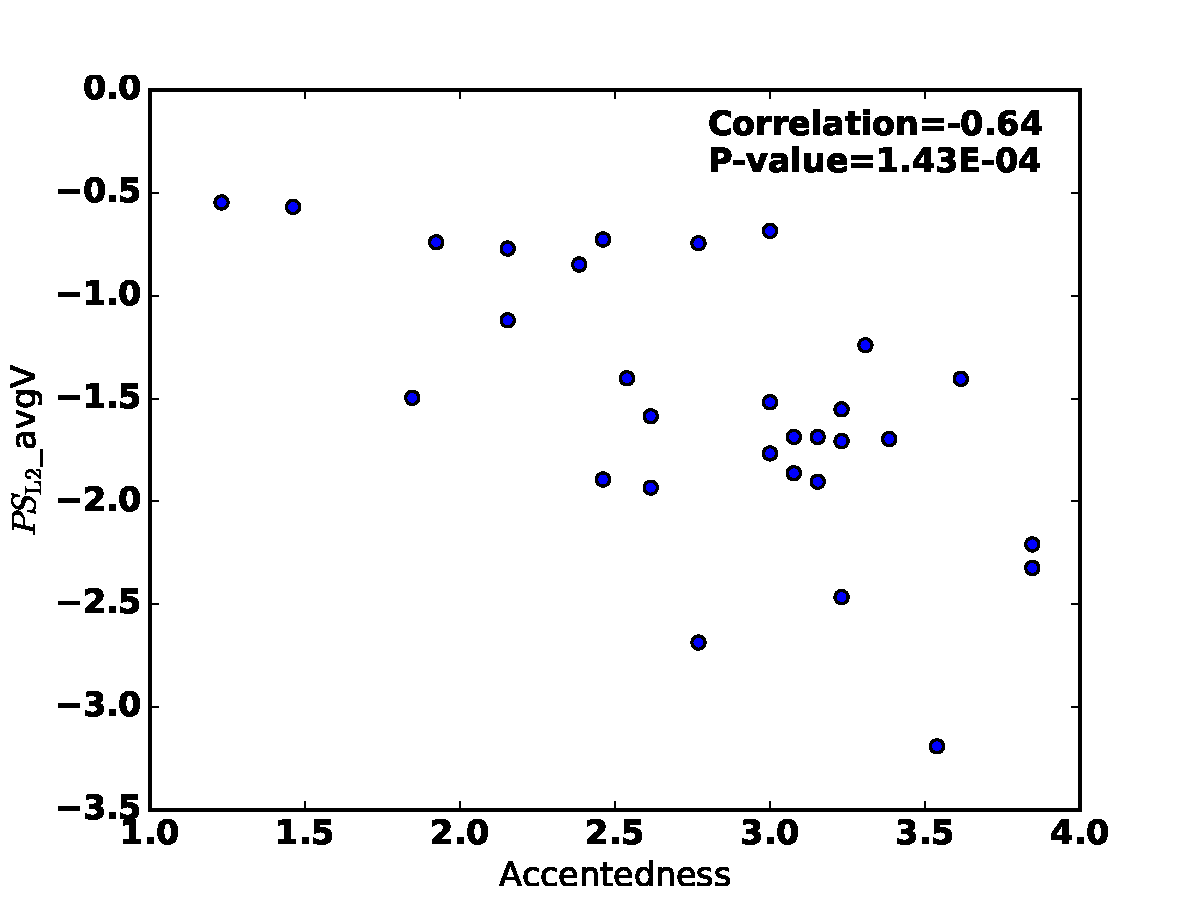
\includegraphics[width=3in]{figures/seg_scatter/figure2_1.pdf}
        \end{minipage}%
        \begin{minipage}[t]{0.5\linewidth}
        \centering
            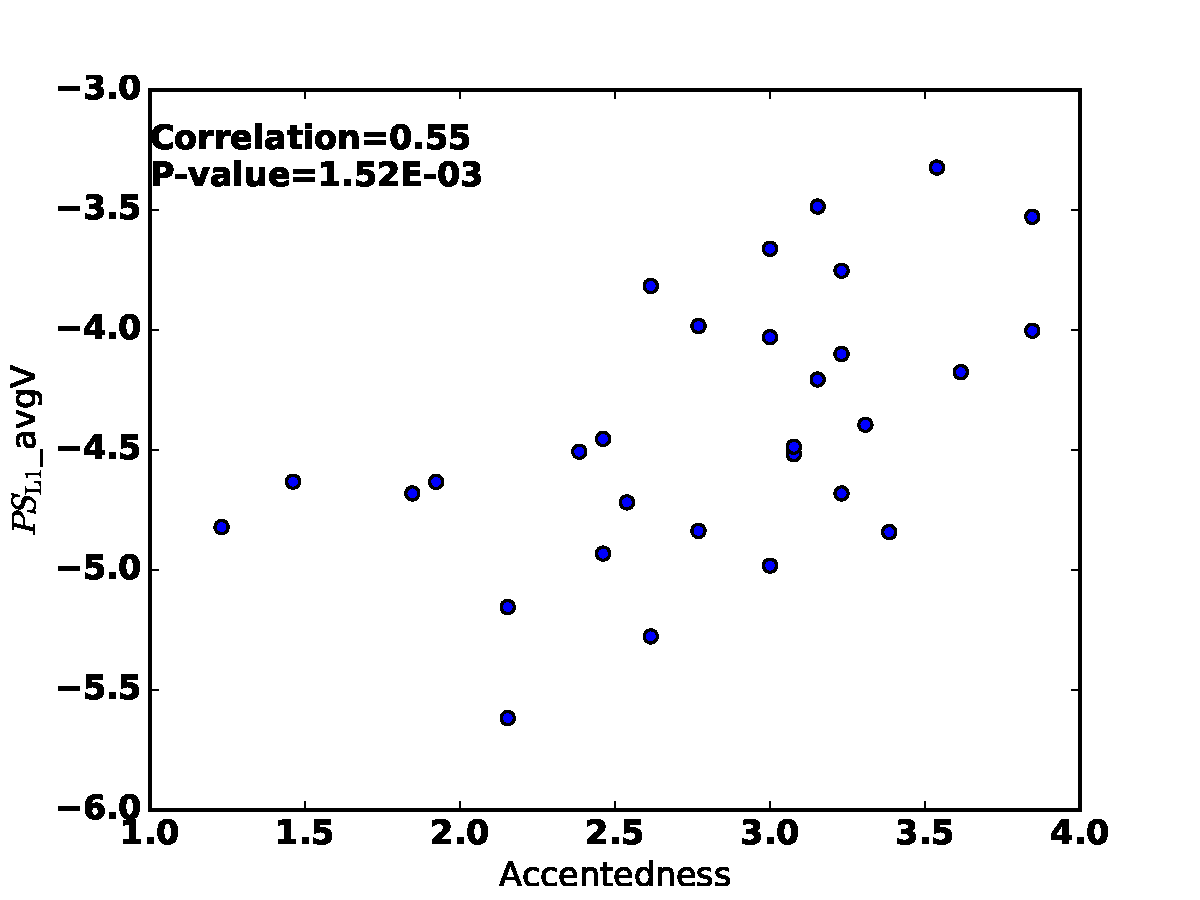
\includegraphics[width=3in]{figures/seg_scatter/figure2_2.pdf}
        \end{minipage}%
        \\
        \begin{minipage}[t]{0.5\linewidth}
        \centering
            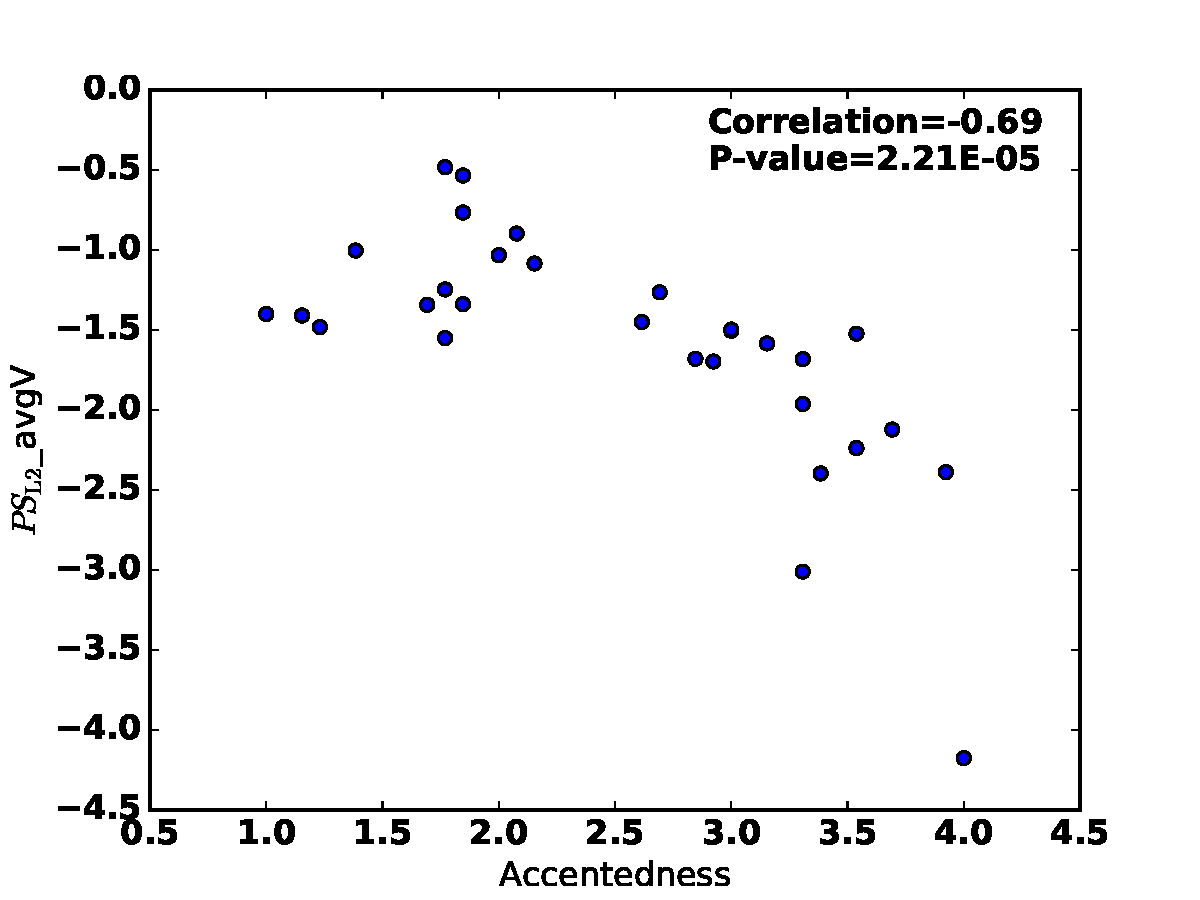
\includegraphics[width=3in]{figures/seg_scatter/figure2_3.pdf}
        \end{minipage}%
        \begin{minipage}[t]{0.5\linewidth}
        \centering
            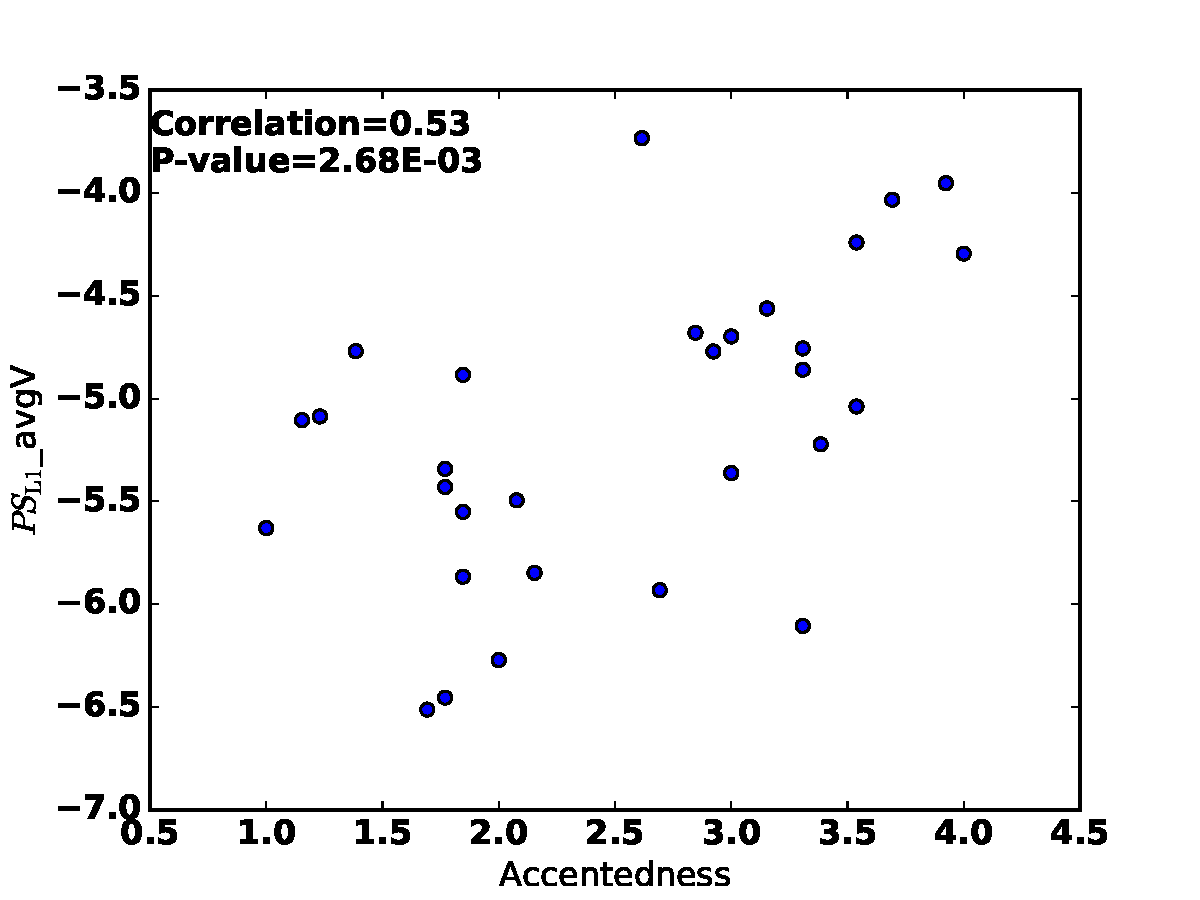
\includegraphics[width=3in]{figures/seg_scatter/figure2_4.pdf}
        \end{minipage}%
        \caption{Scatter plots between accentedness scores and one dimension of features for Mandarin (first row) and Spanish (second row) speakers.}
        \centering
        \label{fig:seg_scatter}
     \end{figure}

\begin{enumerate}
 \item For minimum and average features (row 3 to row 8), the correlations with low p-value (means significantly correlated) achieved with L2 acoustic model are negative while those achieved with l1 acoustic model are positive. This can be interpreted with the physical meanings of the two feature sets. As introduced in section \ref{sec:segmental}, for these pronunciation score based features, higher value means closer to pronunciation patterns model by corresponding acoustic models. Thus, for minimum and average features extracted with L1 acoustic model, higher value means the pronunciation of English is closer to pronunciation patterns of the L1; If a speaker is using the pronunciation patterns of his L1 to produce English, very possibly he has a high accentedness score (towards 4 on the scale); Thus, the correlation coefficients between minimum and average features and accentedness scores are positive. On the contrary, for minimum and average features extracted with L2 English acoustic model, higher value means the pronunciation with accent is closer to pronunciation patterns of native English speakers; Thus, the correlation coefficients are negative. In most cases, the correlation coefficients of minimum features are relatively low while the correlation coefficients of average features are relatively high, which tells that the accentedness score can not be determined by one or two very low pronunciation scores.
 \item For STD features (row 9 to row 11), the patterns are on the other side compared to minimum and average features. This is also easy to interpret: higher STD means there are some very low pronunciation scores; In terms of features extracted with L2 acoustic models, this means possibly higher accentedness score; In terms of features extracted with L1 acoustic models, this means possible lower accentedness score. The correlation coefficients of STD features are also relatively low compared to average features.
 \item STD\_norm features (row 12 to row 14) extracted with L1 acoustic model are not very correlative with accentedness score. However, those extracted with L2 acoustic models can have very high correlation coefficients (such as Mandarin speakers). STD\_norm features are calculated by dividing values of STD features with values of average features. Ideally, it should have same correlational pattern with STD features considering average features and STD features are oppositely correlated with accentedness score.
 \item While the features achieved with L2 acoustic models have higher correlation coefficients with accentedness score, features extracted with L1 acoustic models also show high correlations. This partly support the hypothesis in chapter \ref{introduction} that ``the phonological distance between accented speech and speaker's L1 are negatively correlated with perceived accentedness;''. In figure \ref{fig:seg_scatter}, the scatter plots between average of vowels' PS and accentedness score are presented for Mandarin and Spanish speakers. Based on this observation, it is more likely that when combining features extracted with both L1 and L2 acoustic models can better fit the accentedness score.
\end{enumerate}

\subsection{Results of multiple regression analysis}

In table \ref{table:seg_pred}, both the PCCs and MAEs between model predicted accentedness and human annotated accentedness for 4 groups of speakers are presented. The results of German and French speakers before down-sampling are also showed in the parentheses. There is a clear improvement when adding L1 acoustic model based features for all 4 L1s. These results show that there is an improvement in model performance consistently and across all languages after adding features from the L1 acoustic model. It proves that the L1 contrastive information between accented speech and L1 can provide extra information for accentedness prediction. This is despite the fact that the annotators know little about the acoustic properties of the speakers' L1s.

\begin{table}[t]
\centering
\caption{PCCs and MAEs between predicted accentedness and human scores for speakers of 4 different L1s.}
\label{table:seg_pred}
\begin{tabular}{|c|c|c|c|c|}
\hline
\multirow{2}{*}{} & \multicolumn{2}{c|}{$PS_{\mathrm{L2}}$ only} & \multicolumn{2}{c|}{$PS_{\mathrm{L2}}$ and $PS_{\mathrm{L1}}$} \\ \cline{2-5}
 & PCC & MAE & PCC & MAE \\ \hline
Mandarin & 0.707 & 0.343 & \textbf{0.727} & \textbf{0.329} \\ \hline
Spanish & 0.681 & 0.535 & \textbf{0.730} & \textbf{0.464} \\ \hline
German & \begin{tabular}[c]{@{}c@{}}0.734\\ (0.082)\end{tabular} & \begin{tabular}[c]{@{}c@{}}0.204\\ (0.301)\end{tabular} & \textbf{\begin{tabular}[c]{@{}c@{}}0.833\\ (0.144)\end{tabular}} & \textbf{\begin{tabular}[c]{@{}c@{}}0.163\\ (0.287)\end{tabular}} \\ \hline
French & \begin{tabular}[c]{@{}c@{}}0.531\\ (0.254)\end{tabular} & \begin{tabular}[c]{@{}c@{}}0.335\\ (0.406)\end{tabular} & \textbf{\begin{tabular}[c]{@{}c@{}}0.619\\ (0.411)\end{tabular}} & \textbf{\begin{tabular}[c]{@{}c@{}}0.303\\ (0.370)\end{tabular}} \\ \hline
\end{tabular}
\end{table}

In order to show that features extracted with L1 acoustic model really helps with predicting accentedness scores, in table \ref{table:seg_feat_sel}, L1 acoustic model based features that are selected to predict accentedness scores are showed. Since the multiple regression analyses are done language-independently, different sets of features are selected for different languages, and the number of features selected for each language is also presented in the table. Note that for German and French, the feature selection results are based on subsets of speakers after downsampling. It can be found that for all four languages, the average pronunciation score of vowels, consonants and syllables together with minimum of vowels' pronunciation score and standard deviation of vowels' pronunciation scores are selected. This indicates that the first order information of pronunciation scores extracted with L1 acoustic model can better predict the accentedness score. The results of the multiple regression analysis further validate the hypothesis in chapter \ref{introduction} that ``If this distance information is added to the feature sets for automatic accentedness evaluation, the performance will be improved.

\begin{table}[]
\centering
\caption{Selected features that are extracted with L1 acoustic model for each language. ``num\_feature'' stands for the total number of selected features by feature selection.}
\label{table:seg_feat_sel}
\resizebox{\columnwidth}{!}{%
\begin{tabular}{|c|c|c|c|c|}
\hline
 & German (num\_feat=24) & French (num\_feat=16) & Mandarin (num\_feat=14) & Spanish (num\_feat=14) \\ \hline
\begin{tabular}[c]{@{}c@{}}Minimum of \\ vowels' PS\end{tabular} & Yes & Yes & Yes & Yes \\ \hline
\begin{tabular}[c]{@{}c@{}}Minimum of \\ consonants' PS\end{tabular} & Yes &  &  &  \\ \hline
\begin{tabular}[c]{@{}c@{}}Minimum of \\ syllables' PS\end{tabular} & Yes & Yes &  &  \\ \hline
\begin{tabular}[c]{@{}c@{}}Average of \\ vowels' PS\end{tabular} & Yes & Yes & Yes & Yes \\ \hline
\begin{tabular}[c]{@{}c@{}}Average of \\ consonants' PS\end{tabular} & Yes & Yes & Yes & Yes \\ \hline
\begin{tabular}[c]{@{}c@{}}Average of \\ syllables' PS\end{tabular} & Yes & Yes & Yes & Yes \\ \hline
\begin{tabular}[c]{@{}c@{}}STD of \\ vowels' PS\end{tabular} & Yes & Yes & Yes & Yes \\ \hline
\begin{tabular}[c]{@{}c@{}}STD of \\ consonants' PS\end{tabular} & Yes &  &  &  \\ \hline
\begin{tabular}[c]{@{}c@{}}STD of \\ syllables' PS\end{tabular} & Yes & Yes &  & Yes \\ \hline
\begin{tabular}[c]{@{}c@{}}STD\_norm of \\ vowels' PS\end{tabular} & Yes &  &  &  \\ \hline
\begin{tabular}[c]{@{}c@{}}STD\_norm of \\ consonants' PS\end{tabular} & Yes & Yes & Yes &  \\ \hline
\begin{tabular}[c]{@{}c@{}}STD\_norm of \\ syllables' PS\end{tabular} & Yes &  & Yes &  \\ \hline
\end{tabular}
}
\end{table}

\section{Discussion}

The results in table \ref{table:seg_pred} reveal that the improvement in performance varies across different L1s. There are several possible reasons for this including the different modeling quality of the L1s' ASR systems,  the accentedness annotation quality, or the contribution of articulation features to perceived impressions of accentedness for different languages. Another interesting aspect that is worthy of additional investigation is that although there is knowledge transfer from L1 to L2 during L2 acquisition, this influence can vary across different L1s and even different speakers. For example, some research suggests that there exist some universal effects in L2 learning process that are independent of a speaker's L1 \cite{chang2010first}. The approach in thisstudy may provide a means of comparing L1-specific and L1-agnostic pronunciation errors in an attempt to computationally identify some of the universal effects. Specifically, comparing the L1 and L2 acoustic pronunciation scores of English phonemes produced by L2 learners can indicate which English phonemes are not pronounced well due to the speaker is using a similar way with phonemes in L1 phonetic system (high L1 acoustic model based pronunciation score), and which English phonemes are not pronounced well but they also have low L1 acoustic model based pronunciation score (means the pronunciation pattern has nothing to do with the L1 phonetic system).

It has been shown that the proposed feature sets can boost the performance of accentedness prediction. However, there is still room for improvement. First, as mentioned previously, the GMU speech accent archive dataset has a limited number of speakers and small variation of accentedness for some languages. The recording environment also varies by speaker. A cleaner dataset with uniform accentedness ratings is better suited for our application. Second, the amount and quality of training data for L1 acoustic models can be improved since it is quite limited for some of the languages (Spanish, German and French in this study). More accurate L1 acoustic models may result in an improvement of algorithm performance. Third, it is well known that accentedness is related to both pronunciation and prosodic features. This chapter mainly focuses on pronunciation based features. In the next chapter, the same framework will be extended to speech prosody features.

\chapter{L1's effect on prosodic properties of accented speech}
\label{l1_supraseg}

\section{Introduction}

The previous chapter applies the proposed methodology for accentedness perception to pronunciation based segmental features, and proves that integrating L1 pronunciation information by extracting pronunciation scores of accented English speech with L1 acoustic model can improve the prediction accuracy of accentedness perception. This chapter will focus on apply the same methodology to speech prosodic features to study whether L1 prosodic patterns affect the perception of accentedness. As mentioned in chapter \ref{sec:methodology}, durational rhythmic features will be used as proxy of speech prosody. The methods and analysis of results are almost the same as chapter \ref{l1_seg}. Details will be introduced in following sections.

\section{Methods}

Chapter \ref{sec:methodology} describes the procedure to extract durational rhythmic features. The extracted rhythmic features for native L1, accented L2 speech and native L2 are represented with $\mathbf{x_{L1}}$, $\mathbf{X_{acc}}$ and $\mathbf{x_{L2}}$ respectively. Note that $\mathbf{x_{L1}}$ and $\mathbf{x_{L2}}$ are vectors because they are the average of features extracted from multiple speech recordings. These three sets of features are converted to accent related features by taking the absolute difference between $\mathbf{x_{L1}}$ and $\mathbf{X_{acc}}$ and $\mathbf{x_{L2}}$ and $\mathbf{X_{acc}}$. $\left| \mathbf{x_{L2}}-\mathbf{X_{acc}} \right|$ represent the difference between the rhythmic patterns of accented speech and target L2 speech, while $\left| \mathbf{x_{L1}}- \mathbf{X_{acc}} \right|$ represents the difference between the rhythmic patterns of accented speech and speaker's L1 speech. Here, the subtraction is broadcasted to every row of $\mathbf{X_{acc}}$ to get the contrastive information for each speaker with accent.

The first analysis is the correlation analysis between speech prosodic features and accentedness scores averaged on 13 annotators. Similarity, the PCC is calculated between every features of the 18-dimensional feature vectors in a language-dependent way. The procedure is different from previous chapter observing that the feature dimension is higher than pronunciation features. Thus, only the top-12 features with highest PCC with accentedness scores are shown for each language together with the p-values (lower p-value stands for more statistically significant correlation).

Same multiple regression analysis is done except that the number of input features is changed to 18. Downsampling is not used since it does not help for German speakers. Thus, for each language, multiple regression analysis is conducted between 18-dimensional speech rhythmic measurements and accentedness  scores of 30 speakers. Specifically, $\left| \mathbf{x_{L2}}-\mathbf{X_{acc}} \right|$ is used as the baseline model which only takes the difference of speech rhythmic patterns between accented speech and L2 into consideration. Then, $\left| \mathbf{x_{L1}}- \mathbf{X_{acc}} \right|$ can be combined into the baseline feature set to model the distance between accented speech and L1 on suprasegmental feature space. Finally, input to the baseline model is a 18-dimensional feature vector, and adding L1-related information result in a 36-dimensional feature vector.

As in chapter \ref{l1_seg}, the input feature vectors are first normalized with mean and standard deviation on each dimension. Then, a feature selector based on univariate regression test is applied to select the most predictable features. Ridge regression is used to learn the relationship between input features and accentedness score. The same leave-one-speaker-out CV is employed to evaluate the performance on accentedness prediction. Hyperparameters including number of features selected and strength of 2-norm regularization in ridge regression are tuned to achieve the best CV performance. PCC and MAE are reported language dependently. To better illustrate the process, figure \ref{fig:l1_supraseg_diagram} shows the whole procedure of multiple regression analysis.

\begin{figure}[t]
        \begin{minipage}[t]{1.0\linewidth}
        \centering
            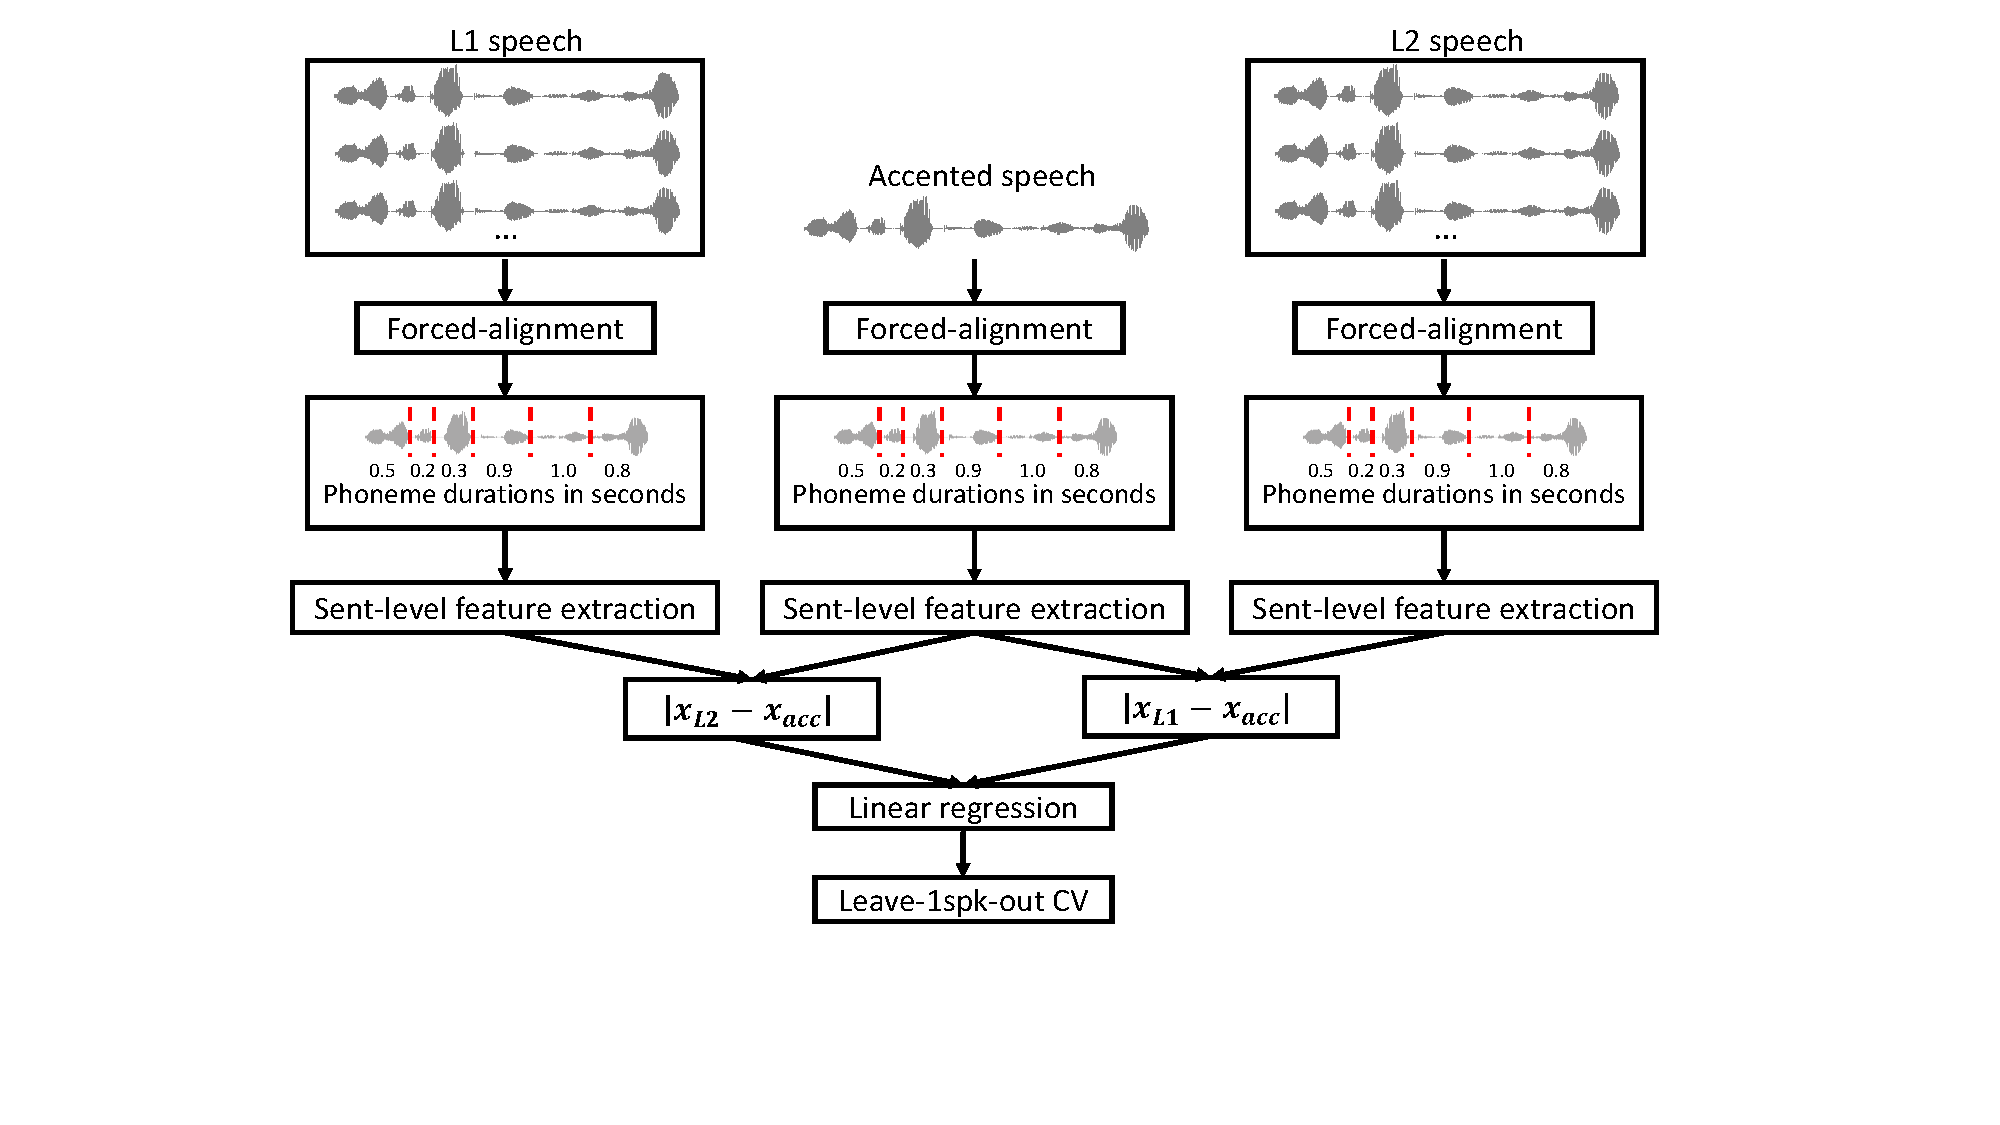
\includegraphics[width=5.0in]{figures/method_diagram_supraseg.pdf}
        \end{minipage}%
        \caption{Diagram of the procedure for multiple regression analysis between suprasegmental prosodic features and accentedness scores. Here, $\mathbf{x_{L1}}$ and $\mathbf{x_{L2}}$ are the average of features of all speech recordings. $\mathbf{x_{acc}}$ is the feature vector for one accented speech recording.}
        \centering
        \label{fig:l1_supraseg_diagram}
     \end{figure}

\section{Results}
\subsection{Results of correlation analysis}

\begin{figure}[]
        \begin{minipage}[t]{0.5\linewidth}
        \centering
            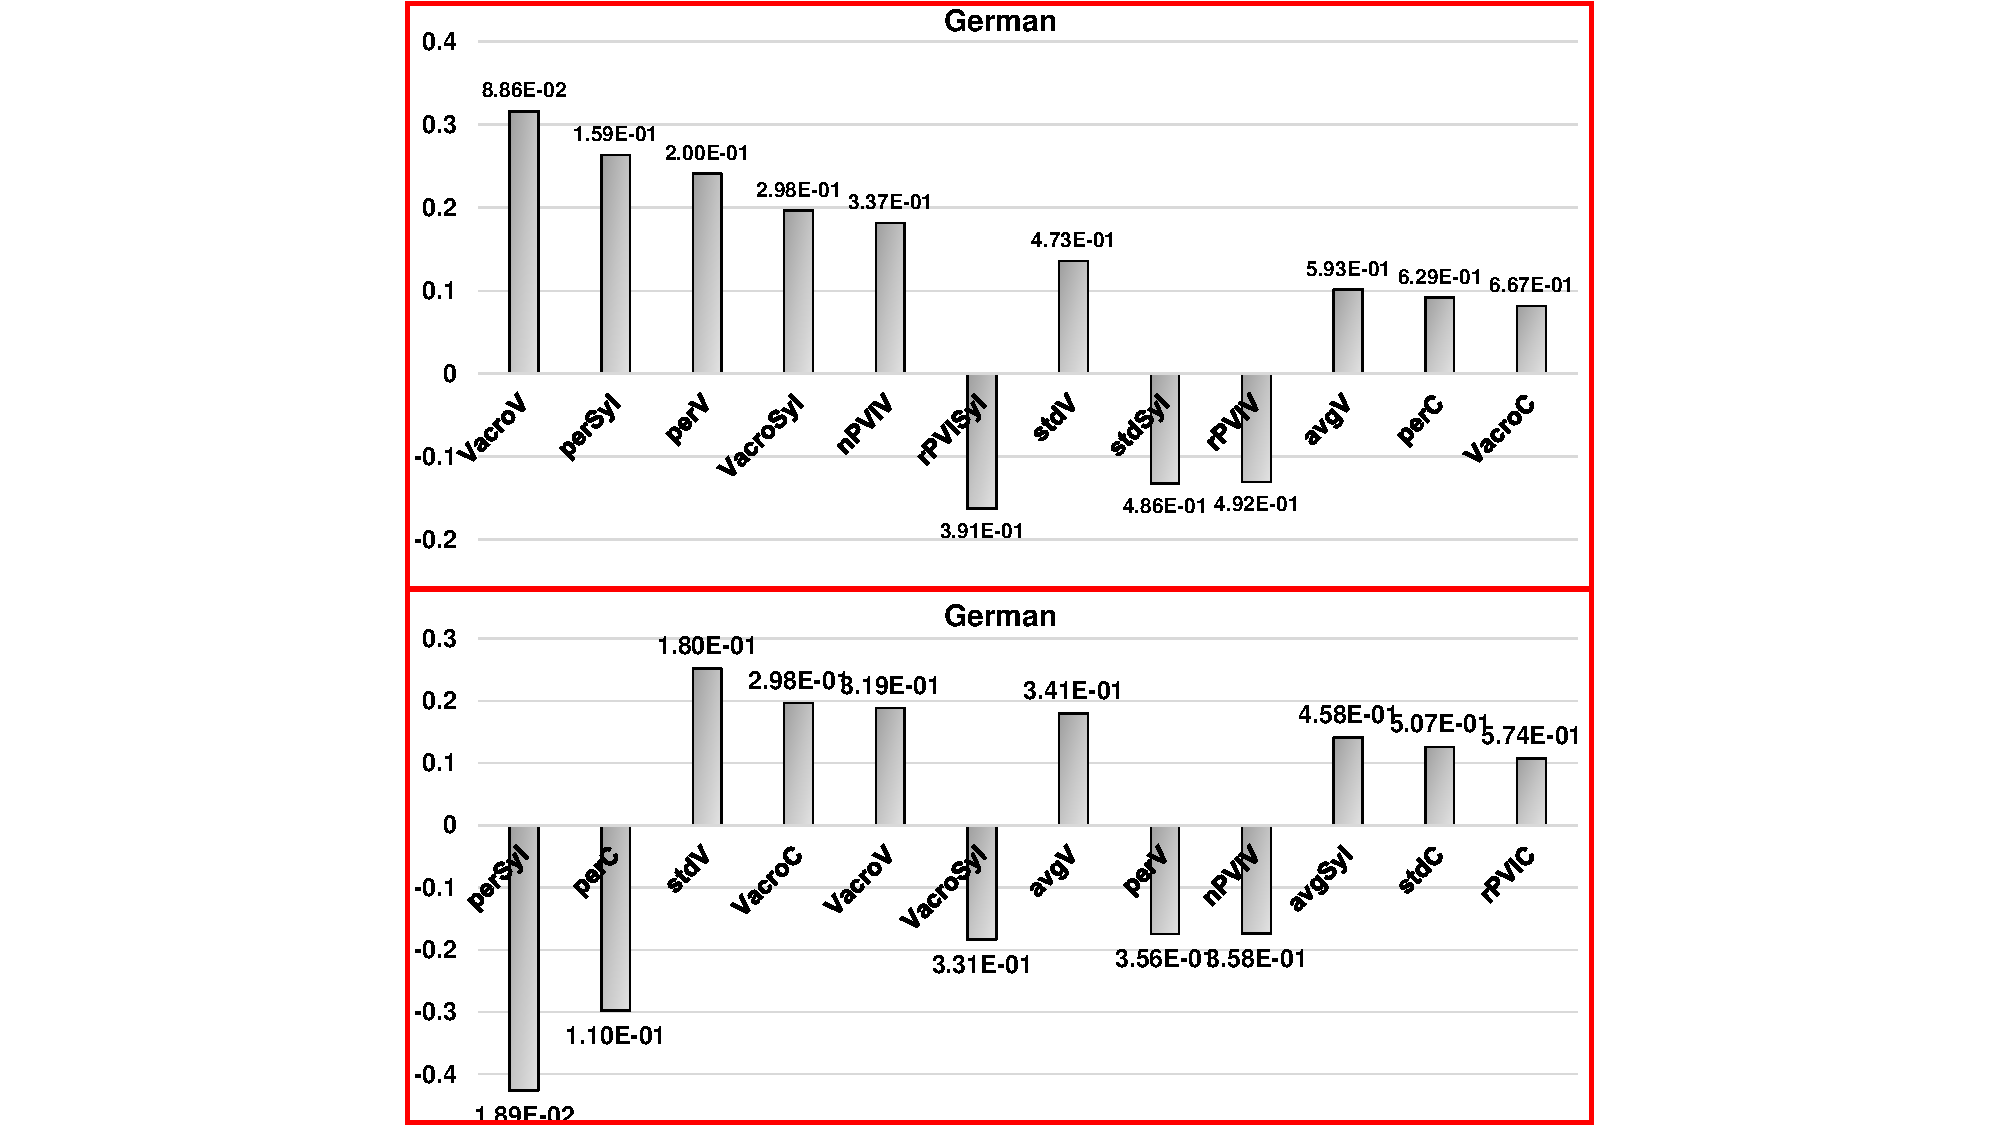
\includegraphics[width=3in]{figures/supra_seg_bar_plot/german.pdf}
        \end{minipage}%
        \begin{minipage}[t]{0.5\linewidth}
        \centering
            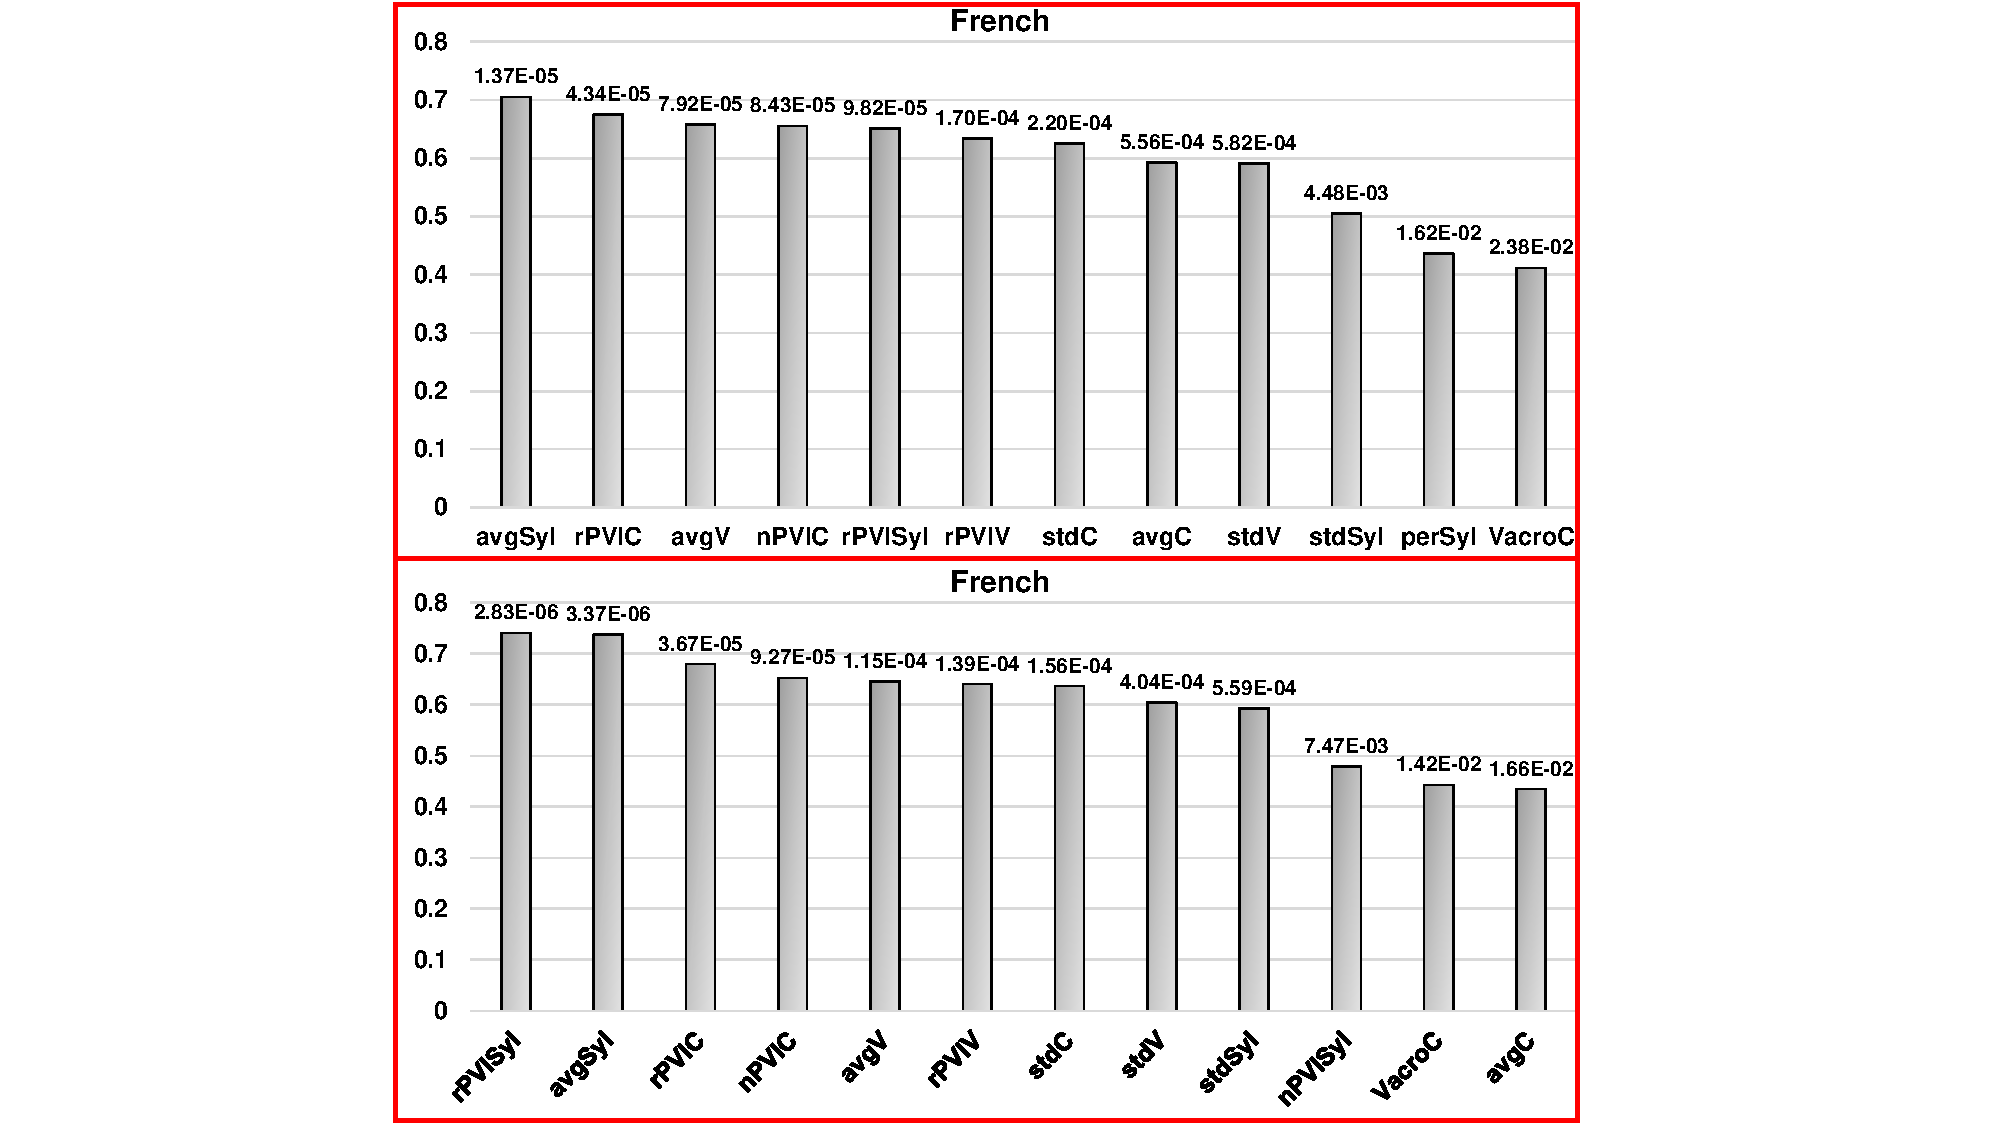
\includegraphics[width=3in]{figures/supra_seg_bar_plot/french.pdf}
        \end{minipage}%
        \\
        \begin{minipage}[t]{0.5\linewidth}
        \centering
            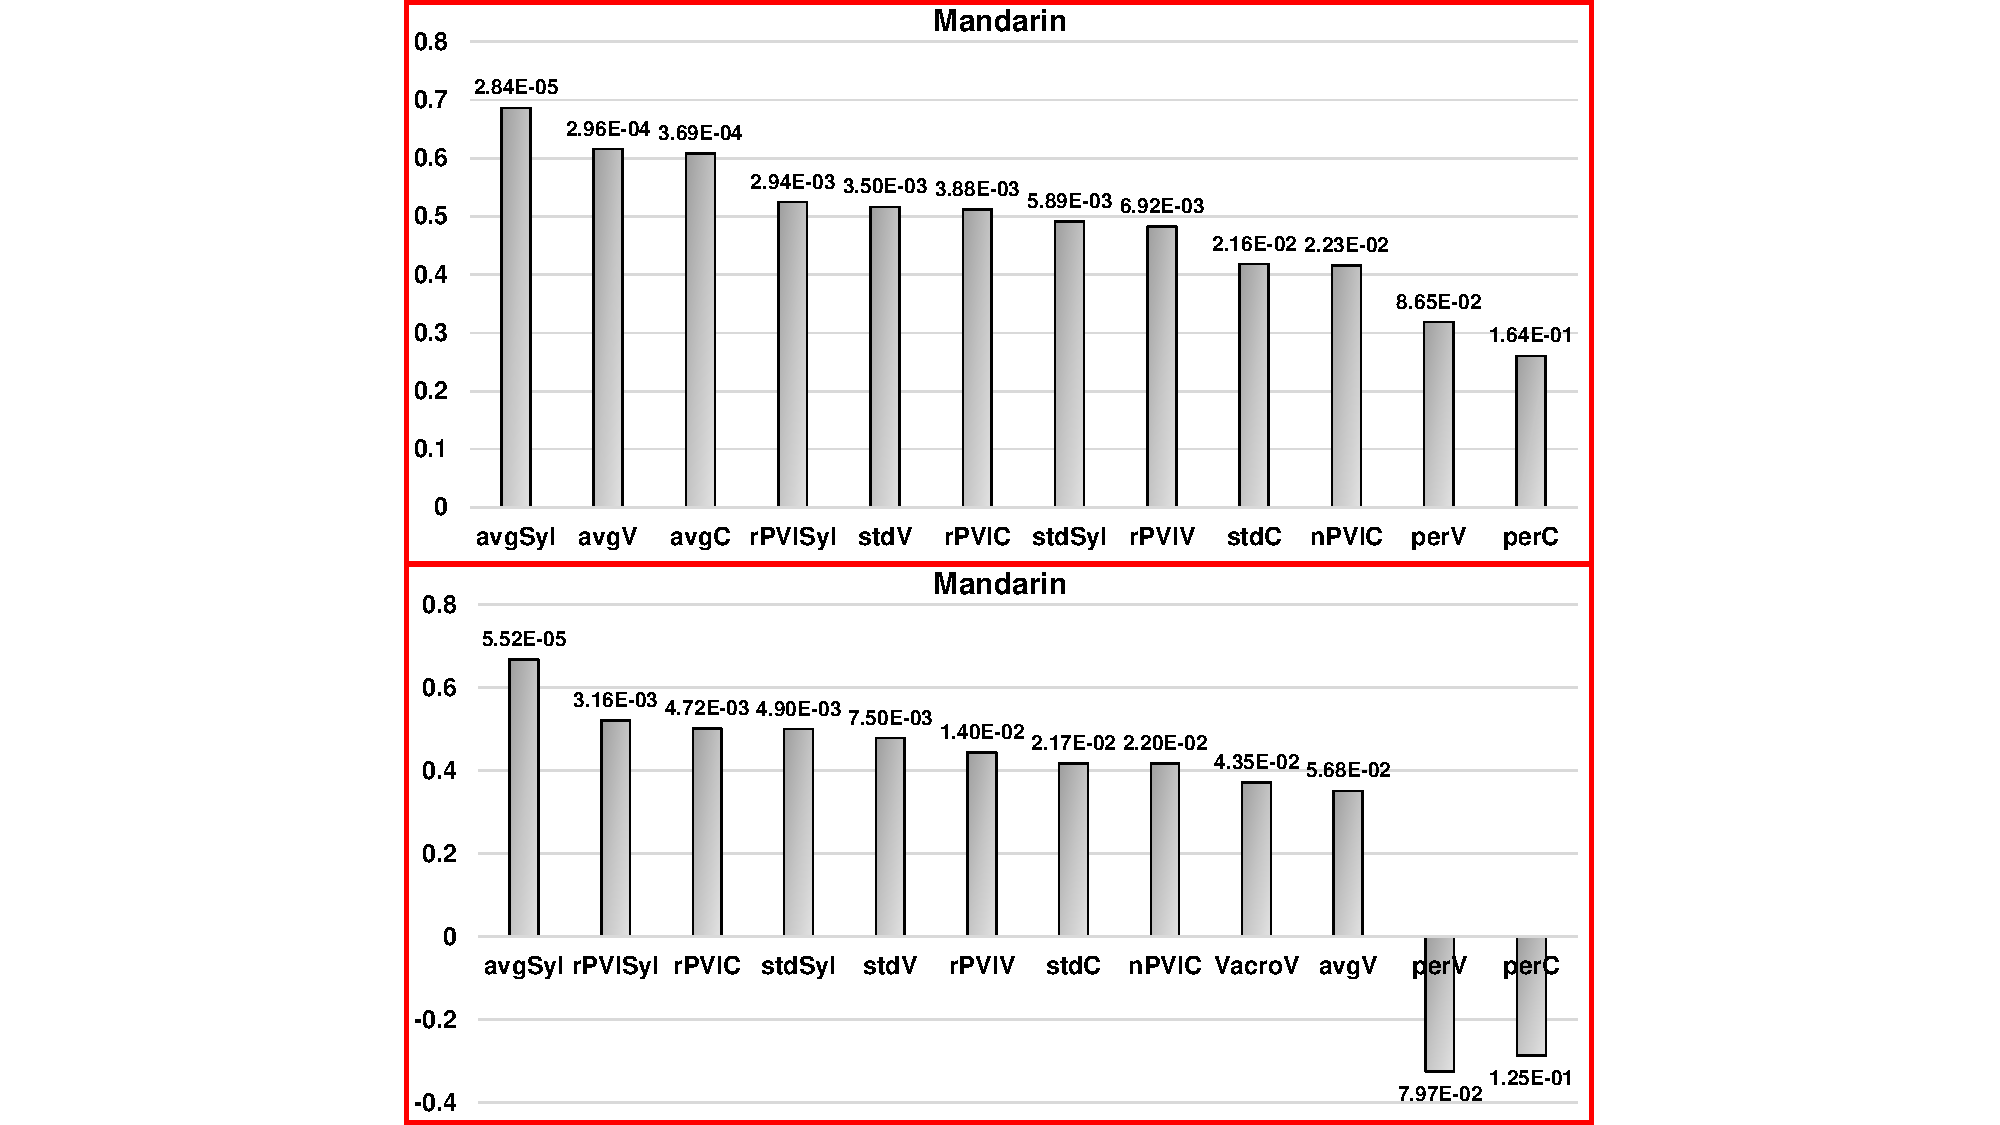
\includegraphics[width=3in]{figures/supra_seg_bar_plot/mandarin.pdf}
        \end{minipage}%
        \begin{minipage}[t]{0.5\linewidth}
        \centering
            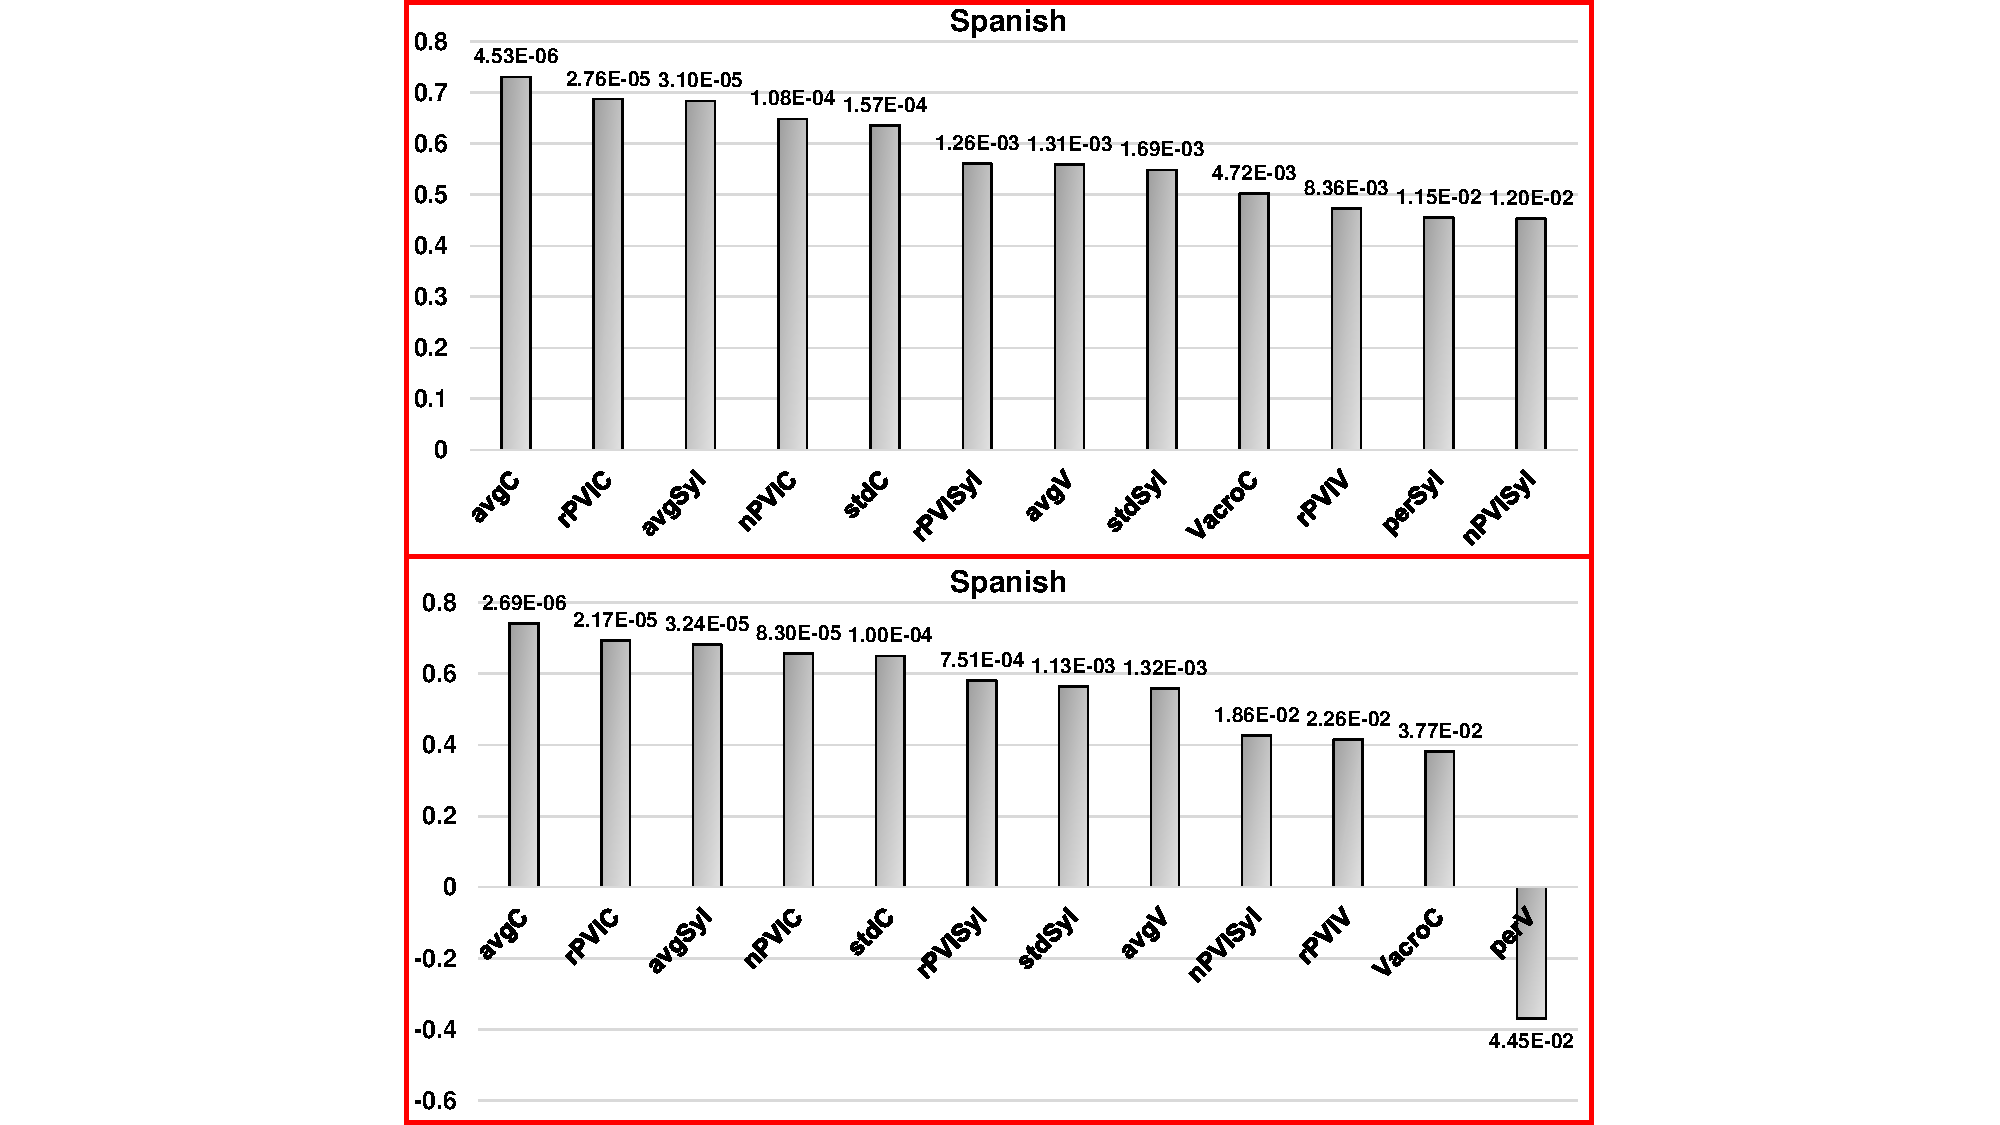
\includegraphics[width=3in]{figures/supra_seg_bar_plot/spanish.pdf}
        \end{minipage}%
        \caption{Bar plots of the top-12 features highly correlated with accentedness scores in feature sets $\left| \mathbf{x_{L2}}-\mathbf{X_{acc}} \right|$ (upper panel in each subfigure) and $\left| \mathbf{x_{L1}}- \mathbf{X_{acc}} \right|$ (lower panel in each subfigure). Y-axis is the correlation coefficients with accentedness score and X-axis is feature names. The numbers on top of each bar are the p-value for testing non-correlation.}
        \centering
        \label{fig:supraseg_bar}
     \end{figure}

In figure \ref{fig:supraseg_bar}, PCC together with p-value between two sets of speech rhythmic features and accentedness scores of four different foreign languages are presented. Feature names on X-axis are abbreviations: per\{V,C,Syl\} represents the percentage of durations of vowels, consonants and syllables, avg\{V,C,Syl\} represents the average durations, std\{V,C,Syl\} represents the standard deviation of durations, Vacro\{V,C,Syl\} represents the mean-normalizd standard deviation of durations, rPVI\{V,C,Syl\} represents the Raw PVI of durations and nPVI\{V,C,Syl\} represents the Normalized PVI) of durations. From the figure, there are several interesting observations:

\begin{enumerate}
\item Except for German speakers, rhythmic features of other three languages all have relatively high correlation coefficients ($>$0.6) with accentedness scores. This can be attributed to the similarity of rhythmic patterns between English and German (as shown in figure \ref{fig:rhythmic_mds} and table \ref{table:conf_rhythmic}, also in the study by \cite{li2014l2}). It becomes hard to use rhythmic features to differentiate between mild and strong accent when the rhythmic patterns of L1 is already very close to L2.
\item As shown in previous chapter, the most predictable features extracted with L1 acoustic models have opposite correlation with accentedness scores compared to features extracted with L2 acoustic models. However, for rhythmic features, it can be found that most features of both $\left| \mathbf{x_{L2}}-\mathbf{X_{acc}} \right|$ and $\left| \mathbf{x_{L1}}- \mathbf{X_{acc}} \right|$ are positively correlated with accentedness scores. Only a few dimensions of $\left| \mathbf{x_{L1}}- \mathbf{X_{acc}} \right|$ have negative correlation with accentedness scores. This indicates that for some speakers, values of feature dimensions in $\mathbf{X_{acc}}$ are not within the range from values of $\mathbf{x_{L2}}$ to values of $\mathbf{x_{L2}}$ in corresponding dimensions, while values on some feature dimensions are between the values in L1 and L2. This is also observed in the study by \cite{white2007calibrating}. This finding is consistent with the founds in \citep{li2014l2} where the authors believe that for speech rhythm acquisition there is a multisystemic model of L2 rhythm acquisition and both transferred L1 knowledge and universal effects independent of L1 played a role.
\item For languages that have high correlation coefficients, it can be found that the average durations features and PVI features are the most correlated ones. This is also consistent with studies by \cite{ordin2015acquisition} where they show the different rhythmic feature values in different proficiency levels: beginners, intermediate and advanced, in spite that they did not provide correlation coefficients between rhythmic feature values and how strong the accent is.
\end{enumerate}

\subsection{Results of multiple regression analysis}

During the experiment, it was found that For French and Mandarin, using feature set [$\left| \mathbf{x_{L2}}-\mathbf{X_{acc}} \right|$, $\left| \mathbf{x_{L2}}-\mathbf{X_{acc}} \right|$-$\left| \mathbf{x_{L1}}- \mathbf{X_{acc}} \right|$] as the way to integrate L1 information gave the best performance of leave-one-speaker-out CV; for Spanish speaker, feature set [$\left| \mathbf{x_{L2}}-\mathbf{X_{acc}} \right|$, $\left| \mathbf{x_{L1}}- \mathbf{X_{acc}} \right|$] gave the best performance. Since for French and Mandarin, using [$\left| \mathbf{x_{L2}}-\mathbf{X_{acc}} \right|$, $\left| \mathbf{x_{L1}}- \mathbf{X_{acc}} \right|$] can also achieve better performance than the baseline model, the difference of the best feature sets across languages is probably due to different speech prosody patterns.
In table \ref{table:supraseg_pred}, both the PCCs and MAEs between model predicted accentedness and human annotated accentedness for 3 groups of speakers are presented. The results for German speakers are not showed because the performance of the regression model is pretty bad, and has negative correlation with human accentedness scores. Downsampling does not help in this case. This is consistent with the correlation analysis in figure \ref{fig:supraseg_bar}, where German rhythmic features have low correlation with accentedness score. There is no downsampling for French speakers either, because without downsampling, the performance on French speakers is already satisfied. There is a consistent improvement when adding L1 rhythmic patterns based features for all 3 L1s. These results show that there is benefit to model performance consistently and across all three languages after adding features from contrastive information with L1 rhythmic patterns. It proves that the rhythmic contrastive information between accented speech and L1 can provide extra information for accentedness prediction. This is also despite the fact that the annotators know little about the acoustic properties of the speakers' L1s.

\begin{table}[]
\centering
\caption{PCCs and MAEs between predicted accentedness and human scores for speakers of three different L1s.}
\label{table:supraseg_pred}
\begin{tabular}{|c|c|c|c|c|}
\hline
 & \multicolumn{2}{c|}{[$\left| \mathbf{x_{L2}}-\mathbf{X_{acc}} \right|$]} & \multicolumn{2}{c|}{With $\left| \mathbf{x_{L1}}- \mathbf{X_{acc}} \right|$} \\ \hline
 & PCC & MAE & PCC & MAE \\ \hline
French & 0.647 & 0.310 & 0.680 & 0.289 \\ \hline
Mandarin & 0.581 & 0.425 & 0.712 & 0.380 \\ \hline
Spanish & 0.698 & 0.507 & 0.729 & 0.482 \\ \hline
\end{tabular}
\end{table}

\begin{table}[]
\centering
\caption{Selected feature dimensions from [$\left| \mathbf{x_{L2}}-\mathbf{X_{acc}} \right|$, $\left| \mathbf{x_{L2}}-\mathbf{X_{acc}} \right|$-$\left| \mathbf{x_{L1}}- \mathbf{X_{acc}} \right|$] for French and Mandarin speakers or [$\left| \mathbf{x_{L2}}-\mathbf{X_{acc}} \right|$, $\left| \mathbf{x_{L1}}- \mathbf{X_{acc}} \right|$] for Spanish speakers. ``num\_feature'' stands for the total number of selected features by feature selection.}
\label{table:supraseg_feat_sel}
\begin{tabular}{|c|c|l|l|l|}
\hline
 & \multicolumn{4}{c|}{Selected feature dimensions} \\ \hline
\begin{tabular}[c]{@{}c@{}}French \\ (num\_feat=25)\end{tabular} & \multicolumn{4}{c|}{\begin{tabular}[c]{@{}c@{}}avgC, avgSyl, stdC, stdSyl,VacroC, \\ perC, perSyl, rPVIC, rPVISyl, nPVISyl\end{tabular}} \\ \hline
\begin{tabular}[c]{@{}c@{}}Mandarin \\ (num\_feat=15)\end{tabular} & \multicolumn{4}{c|}{avgV, avgC, stdV,perV} \\ \hline
\begin{tabular}[c]{@{}c@{}}Spanish \\ (num\_feat=11)\end{tabular} & \multicolumn{4}{c|}{avgC, avgSyl, stdC, rPVIC, rPVISyl,nPVIC} \\ \hline
\end{tabular}
\end{table}

In order to show that features extracted with L1 rhythmic patterns really helps with predicting accentedness scores, in table \ref{table:supraseg_feat_sel} L1 rhythmic patterns based features that are selected to predict accentedness scores are showed. Since the multiple regression analyses are done language-dependently, different sets of features are selected for different languages, and the number of features selected for each language is also presented in the table. It can be found that for French and Spanish speakers, the durational measurements of L1 consonants and syllables are more import features, while for Mandarin speakers the durational measurements of L1 vowels are more import features. The study by \cite{li2014l2} compared durational measurements of Mandarin accented English and native English. They showed that vocalic rhythmic measurements can well discriminate Mandarin learners at different proficiency levels. For French and Spanish speakers, there are no studies showing the progressive change of consonantal and syllable rhythmic measurements along proficiency levels. The results are reasonable considering both French and Spanish are syllable-timed languages while English is stress-timed languages. The results of the multiple regression analysis further validate the first hypothesis in chapter \ref{introduction}.

\section{Discussion}

This chapter shows that the speech prosodic properties transferred from L1 can also help deciding how strong the foreign accent of L2 learners is . This conforms with previous studies, where the authors show the L1's effect on L2 prosody acquisition \citep{rasier2007prosodic,stockmal2005measures,white2007calibrating,li2014l2,ordin2015acquisition}. However, based on the correlation analysis in figure \ref{fig:supraseg_bar}, on most feature dimensions, it does not indicate that if the rhythmic property on that dimension is further from L1, the foreign accent is milder. This is in contrast to the results in table \ref{table:seg_corr}. The first possible reason is that while previous studies show the effect of L1 on L2 rhythmic pattern acquisition, there are also obvious universal effect that are independent of L1. For example, the study \cite{ordin2015acquisition} showed that the PVI measurements of English speech produced by French speakers can be even higher than native English speakers given that English speech has much higher PVI measurements than French speech. The second possible reason is that all the rhythmic measurements in this study are based on automatic forced alignment. For speakers with not very strong accent, there will be much fewer forced-alignment errors. However, for speakers with very strong accent, the forced-alignment results may not be very accurate. This will also affect the correlation analysis between features and accentedness scores. Another interesting observation is that for German speakers, rhythmic features do not help in predicting accentedness score. This is due to the similarity between English and German rhythmic patterns. Both perceptually and computationally, it is hard to find useful rhythmic features extracted from acoustic signal that can discriminate different degrees of foreign accent.

There are also some interesting implications combining the findings in this chapter and chapter \ref{l1_seg}. Compared to the results in chapter \ref{l1_seg}, for German and Mandarin speakers, using only segmental pronunciation based features can better predict accentedness scores than using only supra-segmental rhythmic features; while for French and Spanish, the supra-segmental rhythmic features perform better. This conforms with the language differential analysis presented in chapter \ref{literature}, where it shows the relative distances of different L1s to English on both phonetic space and rhythmic space. 
In contrast to previous studies using phonological properties transplantation to investigate the relative importance of segmental and supra-segmental in accentedness perception, this study provide a new way to look at the same problem with the advantage that this method can provide quantitative analysis. This study further demonstrates that the relative importance of segmental and supra-segmental features may vary according to accented speaker's L1 background, and the variation is due to the contrastive patterns between L1 and L2 in segmental and supra-segmental feature spaces. These findings support the second hypothesis in \ref{introduction}, which claims that ``phonological properties in different subspaces (phonetic or prosodic) of accented speech produced by speakers from different L1 backgrounds will have distinct contribution to perceived accentedness.''.

This study shows that with extra speaker's L1 information, the perception of accentedness can be better modeled compared to only using the deviation from native L2. At first thought, this is against intuition, especially considering the annotators in this study do not know the identify of the speakers's L1, neither can speak those L1s. However, previous study \citep{yuan2010perception} has shown that the accentedness perception of non-native speech by non-native L2 speakers has preference over L1 backgrounds. In the study, eight Mandarin judges who were considered as experienced English speakers were asked to rate the accentedness of speakers speaking eight different L1s. The results showed that Mandarin judges tended to underestimate the accentedness of Cantonese and Mandarin speakers the most, followed by German, Japanese and Vietnamese speakers, and French, Spanish and Russian speakers the least. The authors suggested that structural similarities or differences between the L1 languages of the speakers and the listeners play an important role in the listeners' perception of accentedness. \cite{flege1995factors} reviewed the factors that affecting the perception of accentedness by native L2 speakers. However, since degree of foreign accent is originally defined as the native L2 speaker's perception of deviations from a pronunciation norm that a listener attributes to the
talker not speaking the target language natively \citep{mccullough2013acoustic}, there is no way to study if native L2 speakers have preference depending on the phonological differences and similarities between L1 and L2. This study tends to believe that the difference or similarities on specific phonological dimensions between L1 and L2 play a decisive role in accentedness perception. This effect could vary across speakers instead of simply decided by the distance between averaged L1 phonological patterns and averaged L2 phonological patterns.


\chapter{A computational model for accentedness perception with L1 information}
\label{both_l1_l2}

\section{Introduction}

Chapter \ref{l1_seg} and \ref{l1_supraseg} test the hypotheses of this study in segmental and supra-segmental phonological spaces (represented by acoustic measurements in corresponding spaces). This chapter will use the knowledge derived from previous chapters and propose a new scheme for automatic accentedness evaluation system. The system features a novel feature extraction process, which not only combines both segmental and supra-segmental information but also integrates speakers' L1 information. The way of adding L1 information in this study is also novel in automatic accentedness evaluation literature except for one study. \cite{moustroufas2007automatic} used utterance-level pronunciation scores extracted from both L1 and L2 acoustic models, calculated frame-wise and averaged over the utterance. However, the proposed system has an important difference: the pronunciation scores are calculated on phoneme segments and provide more specific information regarding the accentedness of different phonemic categories. Supra-segmental acoustic measurements representing speech prosody are also included. Furthermore, \cite{moustroufas2007automatic} assume the human evaluator can speak both L1 and L2 and experiments were conducted on only one L1. This study wants to investigate if the L1 acoustic model can help improve prediction even if the human evaluators have no knowledge of the underlying L1. 

To validate the proposed system, dataset introduced in chapter \ref{sec:methodology} will be employed again to conduct experiments on automatic accentedness evaluation both L1-dependently and L1-independently. Same leave-one-speaker-out CV will be used to evaluate the performance of the system. Finally, possible extensions and improvements over the state-of-the-art systems are discussed.

\section{Method}

\begin{figure}[t]
        \begin{minipage}[t]{1.0\linewidth}
        \centering
            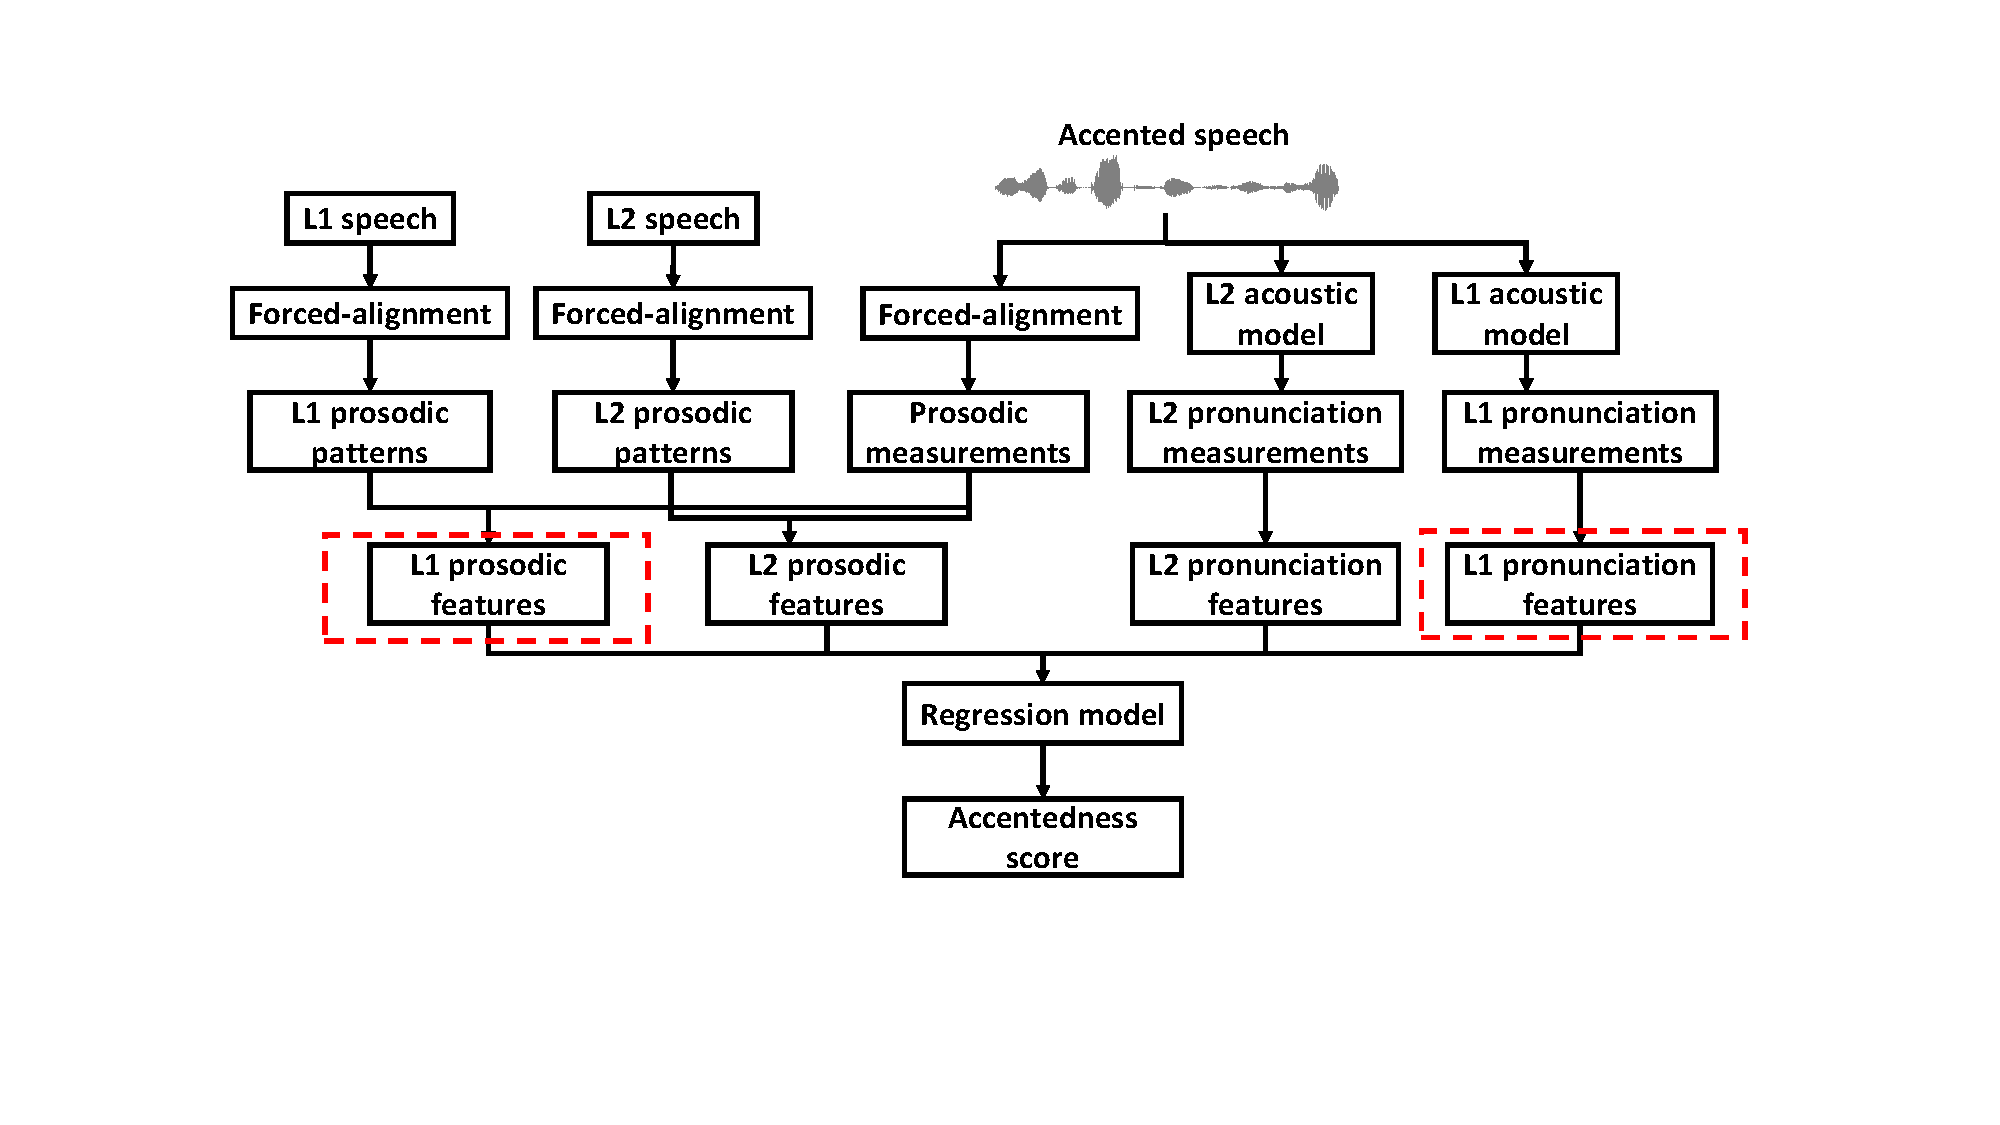
\includegraphics[width=5.0in]{figures/AAE_diagram.pdf}
        \end{minipage}%
        \caption{Diagram of the proposed computational model. The blocks within red box are the highlights of the current model.}
        \centering
        \label{fig:aae_diagram}
     \end{figure}

The diagram of the proposed computational model is shown in figure \ref{fig:aae_diagram}. Prerequisites include a well trained acoustic model (hybrid system built on GMM-HMM or DNN-HMM) on native L2 speech, a well trained acoustic model on native L1 speech, a corpus of native L2 speech for extracting L2 prosodic patterns and a corpus of native L1 speech for extracting L1 prosodic patterns. First, accented speech in L2, native L1 speech and native L2 speech are processed with forced-alignment tools to obtain the durations of each phoneme in the transcripts. There are many available forced-alignment tools with open access \footnote{As summarized in \url{https://github.com/pettarin/forced-alignment-tools}}. Some of them support forced-alignment for multiple languages. For accented speech, usually the forced-alignment performance is inferior compared to native speech because those tools also use acoustic models trained on native speech. To relieve this problem, some recent studies trained the acoustic models for accented speech forced-alignment directly on accented speech to achieve data matching \citep{tao2016exploring, qian2017bidirectional}. However, it requires huge amount of non-native speech recordings which is usually inaccessible. This study employs a forced-alignment tool with an acoustic model trained on a native English speech corpus with about 1000 hours training data to get the phonemes durations of accented speech. After obtaining the phoneme durations of native L1 speech, native L2 speech and accented speech, the feature extraction procedure introduced in section \ref{sec:supraseg} will be applied to get the prosodic patterns of native L1 and L2. This can be achieved by averaging over the sentence-level features over all native L1 and L2 utterances. At the same time, prosodic feature vectors of each accented speech utterances are saved for following process. What previous studies have investigated is that computing the difference between prosodic measurements of accented speech and native L2 speech gives the deviation from native prosodic patterns. This study improves this by using the difference between prosodic measurements of accented speech and native L1 speech to represent how much the prosodic patterns of accented speaker are affected by L1. This results in two sets of feature vectors for each accented speech utterance.

In parallel, accented speech recordings are also sent to both L1 and L2 acoustic models to get the pronunciation scores of each phoneme in the utterance based on the corresponding acoustic model. The algorithms proposed in section \ref{sec:segmental} are used to convert phoneme-level pronunciation score to sentence level pronunciation measurements. Different from previous studies in the literature, this study not only measures the pronunciation mismatch with native L2 speech but also how much the pronunciation in L2 is affected by the speaker's L1. Up to now, there are four feature sets for each accented speech utterance. All of them can be concatenated to form a larger feature vector. Feature vectors without L1 information will be used as baseline system in this study, which has been adopted by recent studies \citep{black2015automated, tao2016exploring, qian2017bidirectional}.

Almost all studies in literature treat the accentedness (or nativeness) evaluation as a regression problem. With the developed sentence-level features, each speaker becomes a data sample with a labeled accentedness score. The accentedness score can be on different scales depending on tasks. This study use a 4-point scale to annotate the accentedness score. Usually, the label will be the average of multiple annotators to reduce inter-rater variability. With feature representation and labels, a regression model can be trained to learn the mapping from input feature to accentedness score. Considering the relatively small number of speakers, this study adopts ridge regression (linear regression with 2-norm regularization) together with a simple feature selection algorithm based on univariate regression analysis. Depending on the dataset, different regression models can be used to achieve better performance. For example, support vector regression \citep{black2015automated}, Gaussian process \citep{grosz2015assessing}, random forest \citep{qian2017bidirectional} and Deep neural networks \citep{grosz2015assessing} are also used in previous studies. SVR is also tried in this study but it is not better than linear regression.

To evaluate the proposed systems, experiments are conducted on both L1-dependent and L1-independent task. For L1-independent task, the system is built on speakers from one L1; for L1-independent task, the system is built on speakers from different L1s. In both cases, leave-one-speaker-out CV is used to evaluate the system's performance because leave-one-out CV is almost the unbiased estimate of generalization error \citep{elisseeff2003leave}. As previous chapters, PCC and MAE on all speakers are used as performance indicators. 

\section{Results}

\begin{table}[t]
\centering
\caption{Performance of accentedness score prediction with different feature sets for different L1s. ``L2\_seg'' stands for L2 pronunciation features. ``+L1\_seg'' means adding L1 pronunciation features to original L2 pronunciation features. ``L2\_supraseg'' stands for L2 prosodic features; ``+L1\_supraseg'' means adding L1 prosodic features to original L2 prosodic features. ``L2\_seg+L2\_supraseg'' represents combining both L2 pronunciation features and L2 prosodic features. ``L1,2\_seg+L1,2\_supraseg'' represents combining all four sets of features together.}
\label{table:ch6_l1_ind}
\resizebox{\columnwidth}{!}{%
\begin{tabular}{|l|c|c|c|c|c|c|c|c|}
\hline
\multicolumn{1}{|c|}{\multirow{2}{*}{}} & \multicolumn{4}{c|}{PCC} & \multicolumn{4}{c|}{MAE} \\ \cline{2-9}
\multicolumn{1}{|c|}{} & German & French & Mandarin & Spanish & German & French & Mandarin & Spanish \\ \hline
L2\_seg & 0.734 & 0.531 & 0.707 & 0.681 & 0.204 & 0.335 & 0.343 & 0.535 \\ \hline
\hspace{0.5cm}+L1\_seg & 0.833 & 0.619 & 0.727 & 0.730 & 0.163 & 0.303 & 0.329 & 0.464 \\ \hline
L2\_supraseg & NA & 0.647 & 0.581 & 0.698 & NA & 0.310 & 0.425 & 0.507 \\ \hline
\hspace{0.5cm}+L1\_supraseg & NA & 0.680 & 0.712 & 0.729 & NA & 0.289 & 0.380 & 0.482 \\ \hline
L2\_seg + L2\_supraseg & NA & 0.667 & 0.733 & 0.846 & NA & 0.308 & 0.319 & 0.404 \\ \hline
L1,2\_seg+L1,2\_supraseg & NA & 0.709 & 0.771 & 0.898 & NA & 0.277 & 0.296 & 0.341 \\ \hline
\end{tabular}}
\end{table}

Table \ref{table:ch6_l1_ind} shows the performance of accentedness score prediction in L1-dependent way with different feature sets. Part of the results is from table \ref{table:seg_pred} and \ref{table:supraseg_pred}. Since the rhythmic features extracted from German speakers can not predict the accentedness score, this table only shows the results for French, Mandarin and Spanish speakers when rhythmic features are included. The results show that when combining both pronunciation and prosodic features, the performance is better than either only using pronunciation features or only using prosodic features. For Spanish speakers, the improvement is the largest. When adding L1 related information to the feature sets, the prediction accuracy is further improved. Again, for Spanish speakers, the PCC is as high as 0.9 (but the MAE is also the highest). This improvement is expected based on the results shown in previous two chapters.

\begin{figure}[t]
        \begin{minipage}[t]{1.0\linewidth}
        \centering
            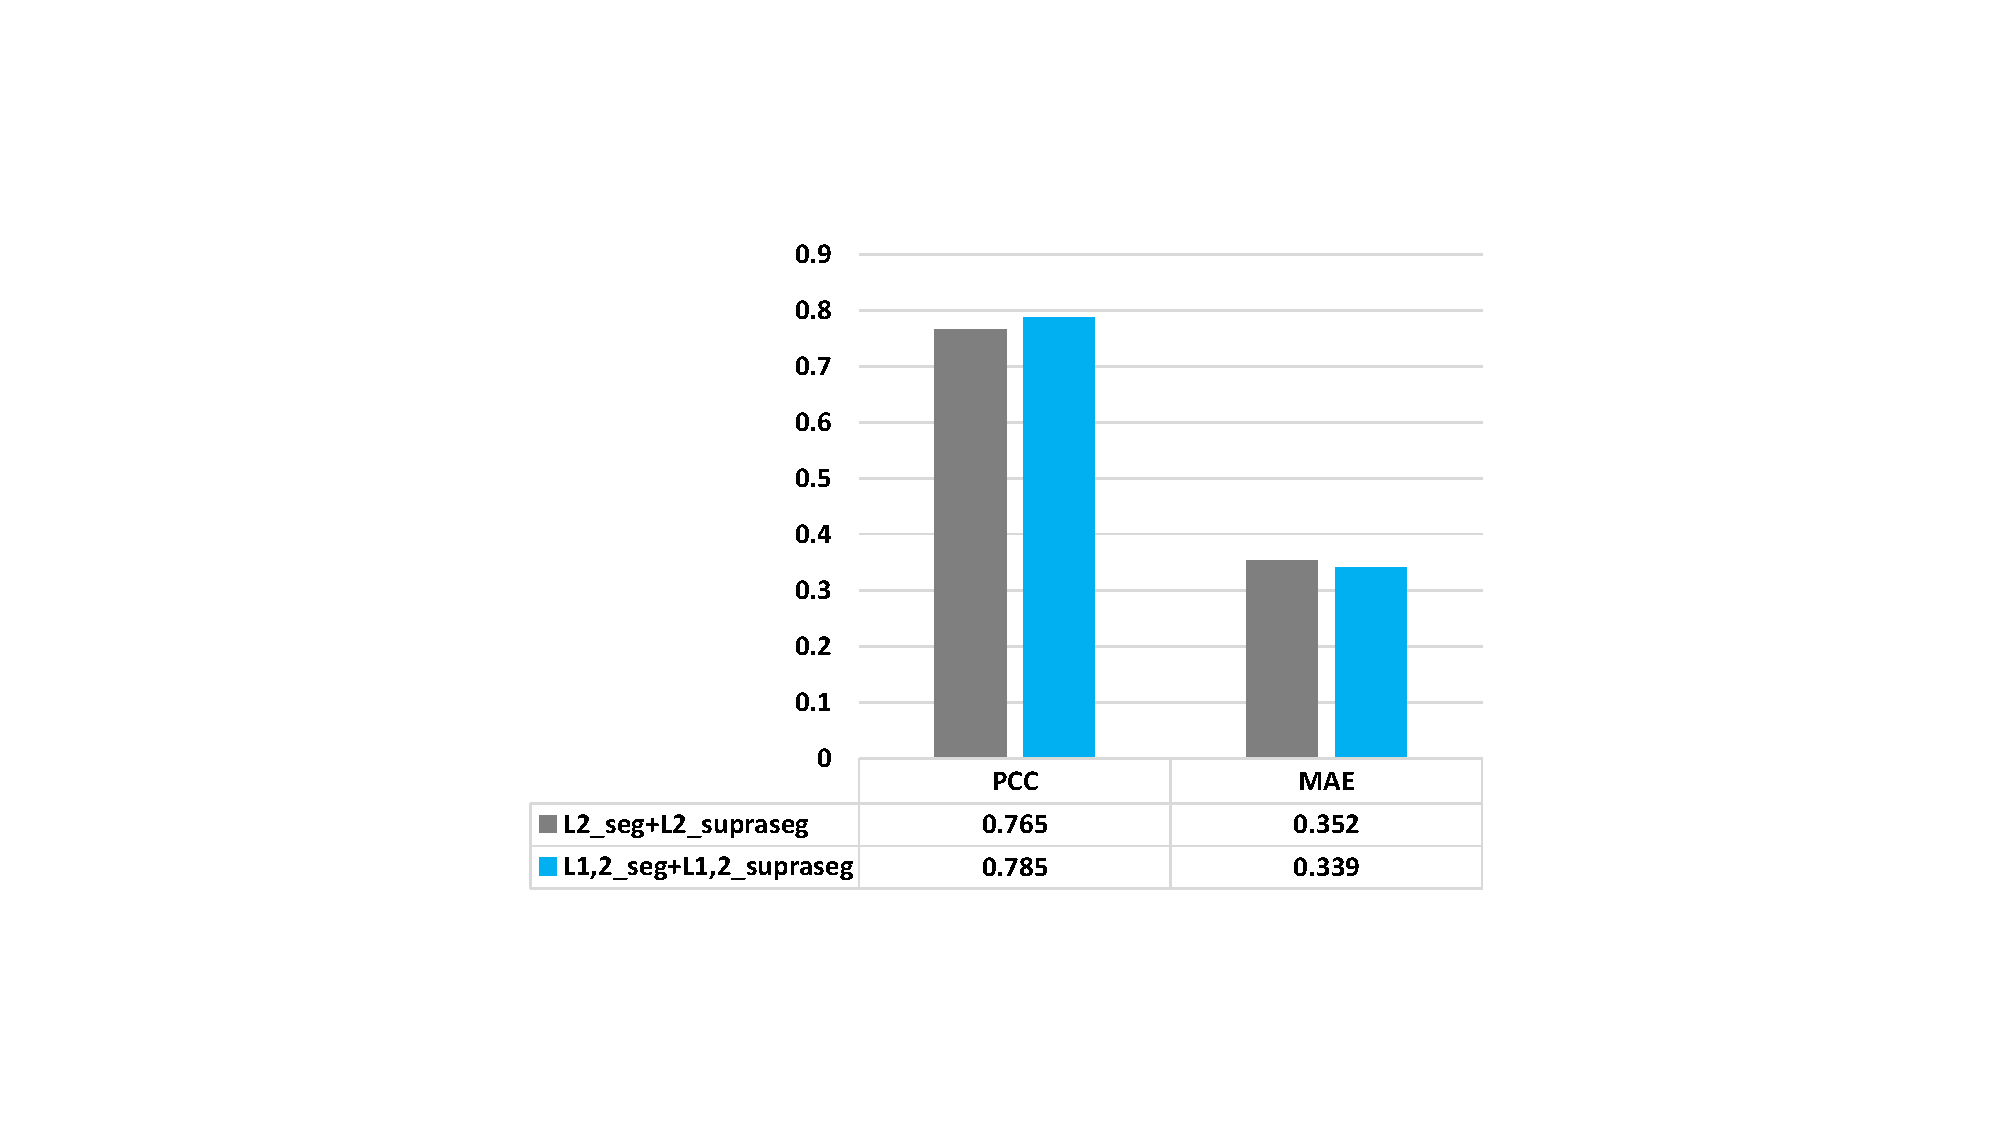
\includegraphics[width=5.0in]{figures/allspk_results.pdf}
        \end{minipage}%
        \caption{Bar plots and detailed values of results in L1-independent way.}
        \centering
        \label{fig:allspk_results}
     \end{figure}
     
\begin{figure}[t]
        \begin{minipage}[t]{1.0\linewidth}
        \centering
            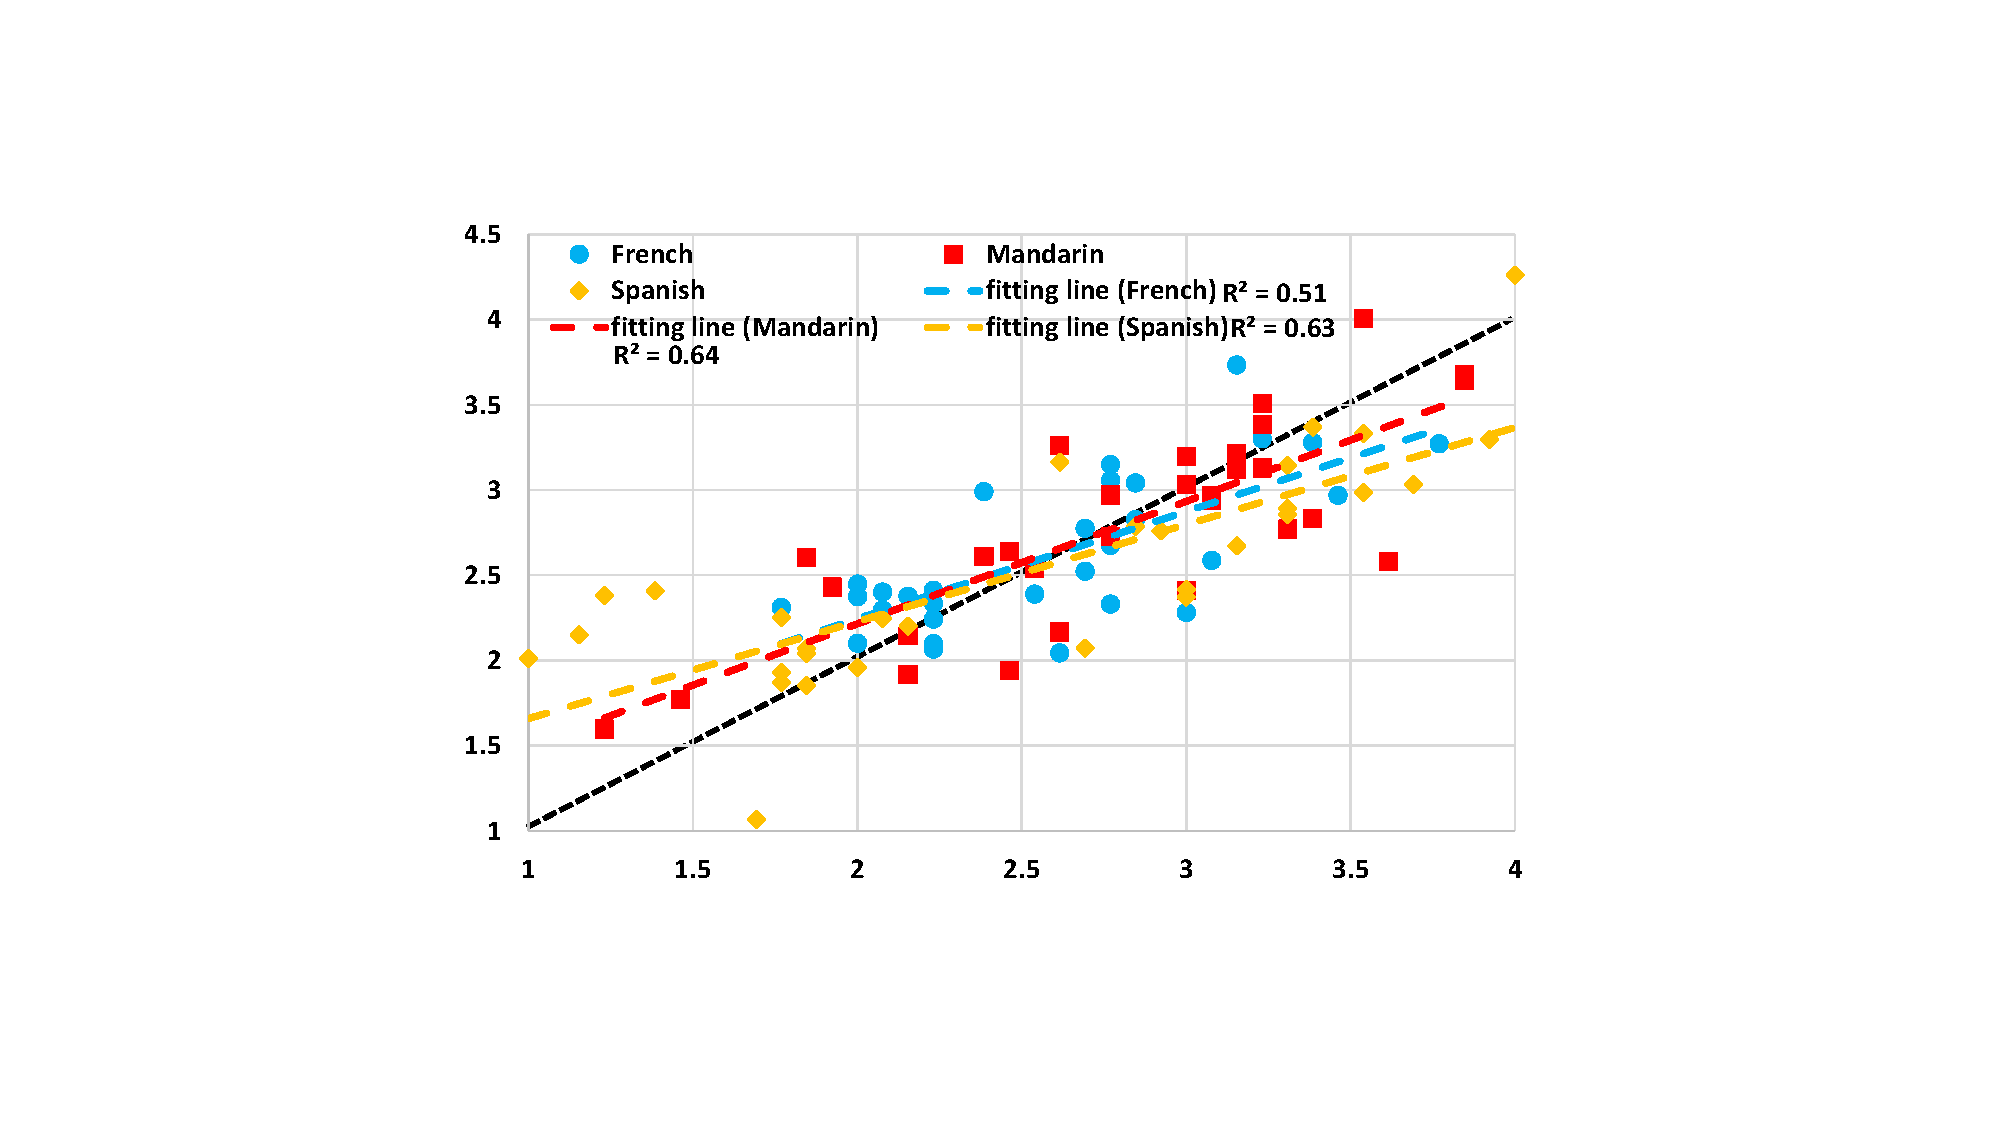
\includegraphics[width=5.0in]{figures/allspk_results_scatter.pdf}
        \end{minipage}%
        \caption{Scatter plots of the true labels and predictions of all 90 speakers from different L1s (French speakers in blue circles, Mandarin speakers in red squares and Spanish speakers in yellow diamonds). X axis is the groundtruth accentedness score and Y axis is the prediction. The fitting line for each L1 is also shown here together with the perfect fitting line (black dash line). R square values are also presented.}
        \centering
        \label{fig:allspk_results_scatter}
     \end{figure}

Figure \ref{fig:allspk_results} shows the results when all speakers from French, Mandarin and Spanish are taken into account. Again, German speakers are excluded because prosodic features are also included. Marginal improvement can be observed when adding L1 related features to the input. It proves that the L1 related information can also help the prediction in L1-independent case. However, it can be found that the improvement in L1-independent experiment is less than the improvement in L1-dependent experiment. The reason for this will be discussed in next section. Since the improvement is not that large, figure \ref{fig:allspk_results_scatter} only shows the scatter plot of the results achieved with all four feature sets. Speakers from different L1s are plot in different colors together with the fitting lines. It can be found that the fitting line of Mandarin speakers is the closest to the perfect fitting line and with the highest R square value. The figure also shows that there are more data samples in the middle range (1.7 to 3.5) on the 4-point accentedness scale. As a result, the fitting is better in that range. However, since there are less data samples at the two ends on the accentedness scale, the fittings there are worse.

\section{Discussion}

This chapter derives a computational model for automatic accentedness evaluation based on findings in previous chapters. The core idea is a new feature extractions scheme that not only quantifies the deviation from native L2 phonological patterns but also how much the accented speech is affected by L1 phonological patterns. Experiments on both L1-dependent and L1-independent tasks show that there is consistent improvement when combining L1 information in the input feature sets.

As a computational model, some blocks of the proposed system can be flexible depending the specific task and resources available. For example, more powerful acoustic models can be used to derive better pronunciation features. More accurate forced-alignment can also be achieved with better forced-alignment tools, thus improving the prosodic features. Depending on the size of dataset, regression models with different complexity can be applied to achieve better performance. Although the evaluation in the current study is done on speaker-level, the proposed framework can be easily extended to sentence-level evaluation.

As mentioned before, the performance improvement of the proposed system on L1-independent tasks is smaller than L1-dependent tasks. This is due to the variability introduced by different L1 acoustic models and different forced-alignment tools for different L1s. This may result in the scales of L1 related features variate for different L1s. This problem can be relieved by using equally powerful L1 acoustic models and forced-alignments, although it could cost much more effort. Another possible way is to normalize the L1-dependent features with the distance between L1 and L2 pronunciation patterns or the distance between L1 and L2 prosodic patterns. It is not easy to directly calculate the distance between pronunciation patterns of two language given their acoustic models. This study tried to normalize the L1 prosodic measurements with the distance between prosodic patterns of L1 and L2, which almost does not change the final results. This is possibly because there is too much variation of the forced-alignment quality of different L1s. However, this study still believe this is a direction worth more investigation.

\chapter{General discussion}
\label{discussion}

\section{Introduction}

This chapter provides a general discussion about the experiments and findings in this study. Specially, both theoretic and practical implications of the current study will be introduced. The first section will focus on how the current study contributes to L2 learning theories, and the second section will focus on how the current study contributes to automatic accentedness evaluation.

\section{Implication for second language learning theories}

As reviewed in chapter \ref{literature}, a bunch of studies have investigate the effect of L1 in the acquisition of L2 phonological properties. This effect presents in both segmental (ash shown by \cite{strange1992learning, flege1987production, chang2008phonetic, munro1993productions, derakhshan2015interference}) and suprasegmental acquisition (as shown by \cite{mennen2004bi, stockmal2005measures, white2007calibrating, lin2008interlanguage, li2014l2, ordin2015acquisition}). However, for segmental properties acquisition, almost all previously mentioned studies have several limitations to comprehensively reveal the detail about the L1's effect on L2 acquisition:

\begin{enumerate}
\item Almost all studies only focus on a specific phonological phenomenon, and analyze how L1 affect the production in L2.
\item Usually the numbers of analyzed speakers and L1s are quite limited.
\item Those studies can only show the L1's effect exist, but there is no way to quantize the influence of L1.
\end{enumerate}

For suprasegmental properties acquisition, thanks to the study by \cite{ramus1999correlates,grabe2002durational}, several publications use durational rhythmic measurements to show the change of those measurements at different stage of L2 learning. However, these studies still have the similar limitations that the numbers of L1s and speakers per L1 are small. Moreover, no quantified speakers' accentedness scores are available in those studies, only some qualitative ranges (for example, from beginners to advanced learners).

Different from the methodology presented in previous work, the current study proposes to use a computational framework to quantify the L2 learning outcomes of tens of speakers from multiple L1s. Both segmental and suprasegmental phonology acquisition are investigated. The analyses done in this study further validate that the influence of L1 exists in both segmental and suprasegmental phonology acquisition during L2 learning. More importantly, with the L1s' information, multiple regression analysis reveals that the accentedness can be better perceived. Besides this, the current study further shows that the difference originates from speakers' L1s will also be presented in their accented speech through the analysis of relative contribution of segmental and supra-segmental features to accentedness scores. In the following, Mandarin speakers will be taken as examples to illustrate how the methodology proposed by this study can be further utilized to investigate the L2 learning process.

\begin{figure}[t]
        \begin{minipage}[t]{1.0\linewidth}
        \centering
            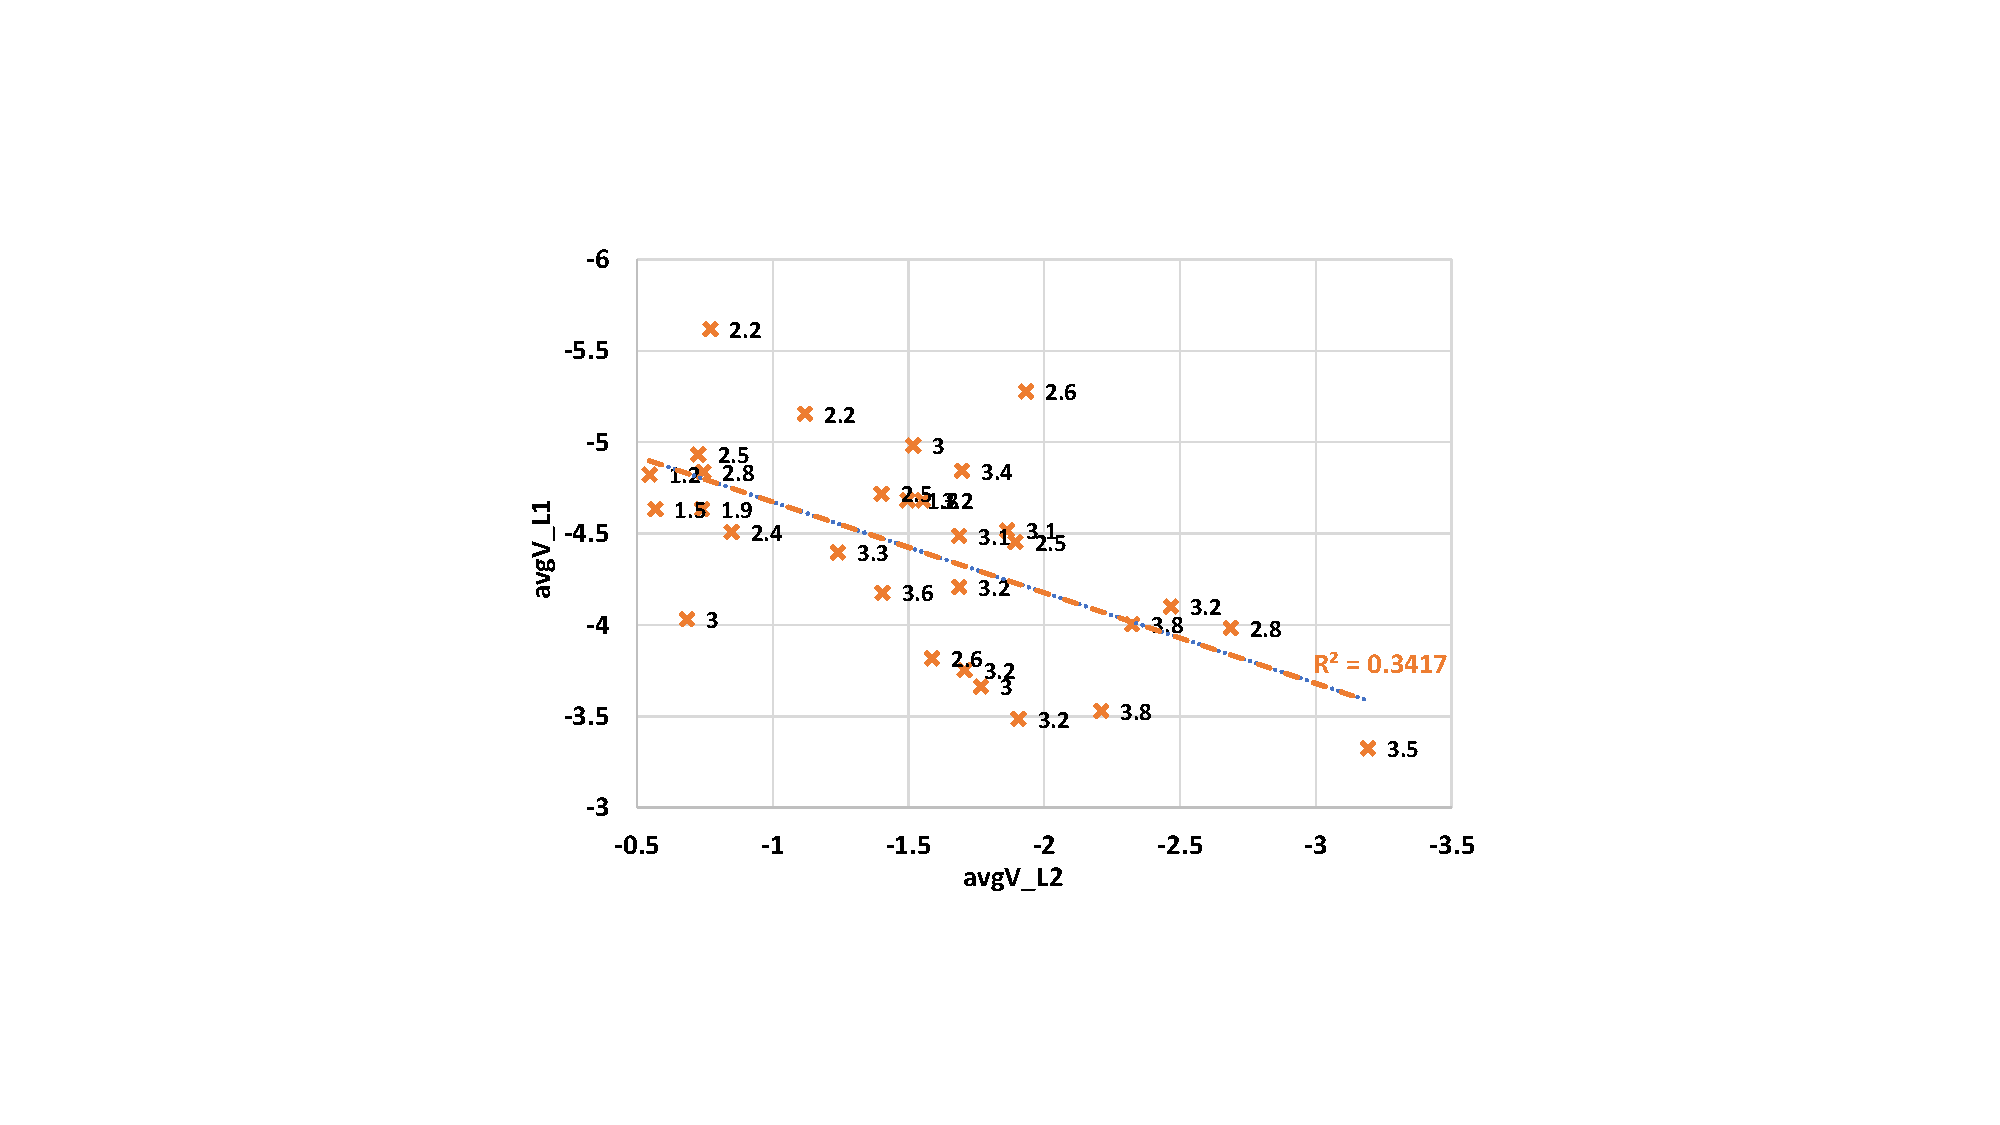
\includegraphics[width=5.0in]{figures/ch7_seg.pdf}
        \end{minipage}%
        \caption{The average pronunciation scores of vowels in accented speech by Mandarin speakers using both L2 (X-axis) and L1 (Y-axis) acoustic models. Larger pronunciation score means closer vowel pronunciation to the pronunciation pattern defined by corresponding acoustic model.}
        \centering
        \label{fig:ch7_seg}
     \end{figure}

Figure \ref{fig:ch7_seg} shows the average pronunciation scores of vowels in accented speech by Mandarin speakers using both L2 (X-axis) and L1 (Y-axis) acoustic models. Each speaker (a cross in the figure) has an average vocalic pronunciation score calculated from L2 acoustic model (avgV\_L2), and the other one (avgV\_L1) is calculated from L1 acoustic model. Larger pronunciation score means closer vowel pronunciation to the pronunciation pattern defined by corresponding acoustic models. The accentedness score of each speaker is also shown along with the crossing on the scatter plot. As shown in figure \ref{fig:seg_scatter}, the avgV\_L2 has a negative correlation with accentedness score while avgV\_L1 has a positive correlation. In order to better show the L1's effect on L2 pronunciation for speakers at different point on the accentedness scale, this figure plots how similar each speaker's L2 pronunciation is with native L2 and native L1, and together with the accentedness scores. There are several interesting findings in the figure. First, the orange dash line demonstrates the general trend that if one speaker's L2 pronunciation is closer to native L2 speaker, his avgV\_L1 score will be lower (means further from L1 pronunciation). Second, it can be found that very accented speakers are at the lower-right corner while mildly accented speakers are at the upper-left corner. However, pronunciation can not explain all the variations of accentedness, as indicated by some outliers. For example, two speakers (one with 2.8 accentedness score and the other 3.0) has good pronunciation but are still considered to have strong accented. Third, since the pronunciation score is calculated as the similarity between accented speech and native speech, the positions of native L1 and L2 can not be put on this scatter plot. The L2 can be considered to have 0 avgV\-L2 value but the avgV\_L1 value can not be decided using the current computational model (similar for L1). However, given enough number of speakers, the distance between L1 and L2 can be approximated by the avgV\_L1 values of speakers with mildest accent. Fourth, another observation is that there are some obvious outliers which are not right on the transferring path from L1 to L2. For example, both the avgV\_L2 (around -1.9) and avgV\_L1 (around -5.3) values of the speaker with 2.6 accentedness score 2.6 are relatively low. Those outliers can be attributed to the universal effects mentioned in previous studies (as reviewed by \cite{white1989universal}) which claim a learner's L2 system have traits that are neither related to L1 nor L2. Also, \cite{major1987model} also found that the amount of L1's influence decreased as learners become more proficient in L2, and this behavior may vary for different learners.

\begin{figure}[t]
        \begin{minipage}[t]{1.0\linewidth}
        \centering
            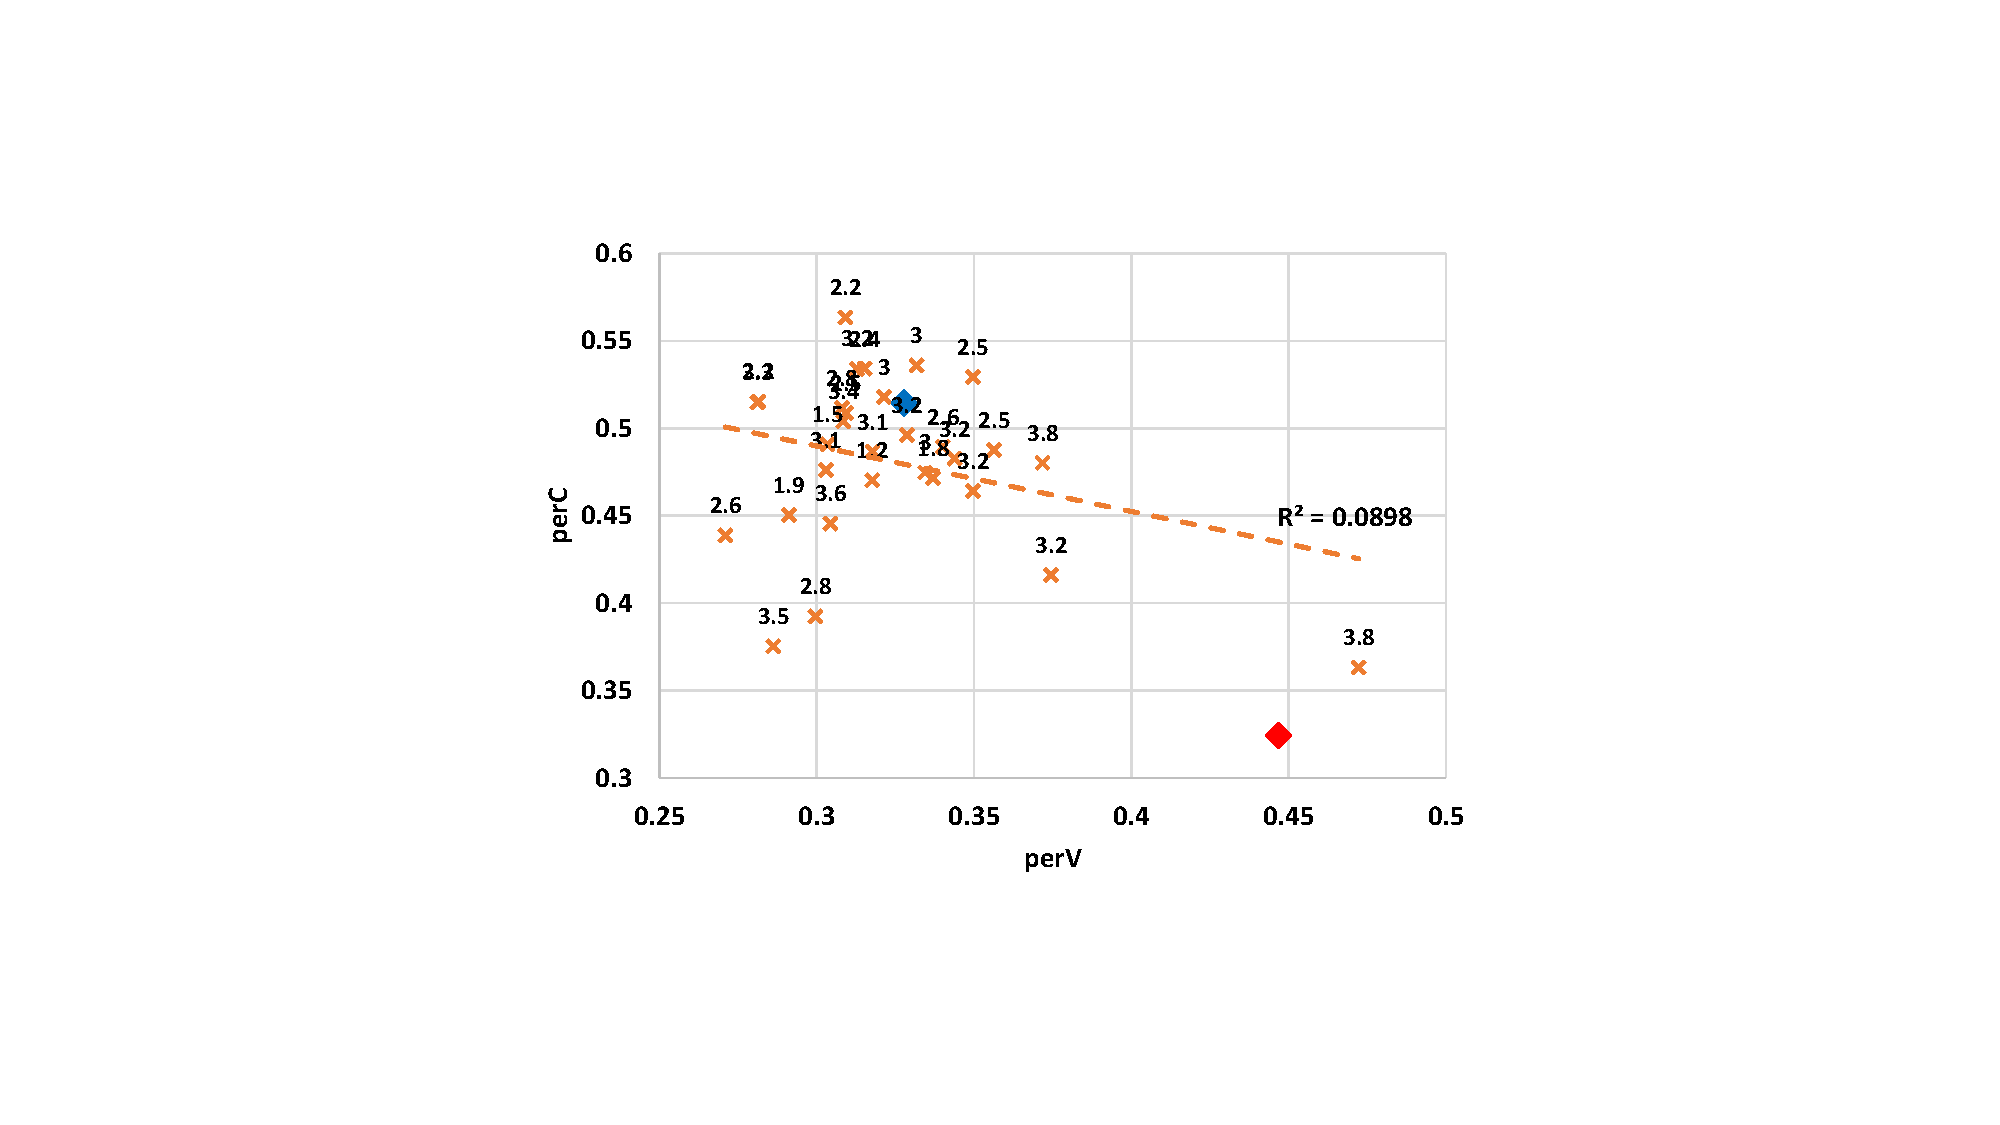
\includegraphics[width=5.0in]{figures/ch7_supraseg.pdf}
        \end{minipage}%
        \caption{Scatter plot of two rhythmic measurements of accented speech by Mandarin speakers: percentage of vocalic (X-axis) and consonantal (Y-axis) durations. The measurements of native English (Blue diamond) and Mandarin (Red diamond) are also shown.}
        \centering
        \label{fig:ch7_supraseg}
     \end{figure}

Figure \ref{fig:ch7_supraseg} demonstrates the scatter plot between two speech rhythmic measurements: the percentage of vocalic and consonantal durations extracted from Mandarin speakers. These two measurements are chosen because they show more L1's effect for strong accented speakers. X-axis is the percentage of vocalic duration (perV) and Y-axis is the percentage of consonantal duration (perC). Since these measurements are absolute values, both the values of L1, L2 and accented speech can be calculated independently. In the figure, the blue diamond is the position of native English; the red diamond is the position of native Mandarin; the orange crossings are accented speakers. The trend line (orange dash line) and R-square value are on the accented speakers only. Compared to English, Mandarin has high perV value but lower perC value. It can be found that measurements of most of accented speakers are around the native English, and only part of them are on the path from native L1 to native L2. This observation is in line with previous studies on L2 speech rhythm acquisition \citep{li2014l2,lin2008interlanguage} where the authors show evidences that speech rhythmic measurements are not on the path from L1 to L2, indicating existence of effects that are independent from L1. However, the speaker with the highest accentedness score (3.8) clearly uses the L1 patterns to pronounce English. The results suggests that the prosodic patterns of accented speakers can be affected by L1, but may only influence a few prosodic dimensions or even be independent from L1.

To summarize, besides the conclusions drew by this study, it is expected that the methodology used in this study could facilitate further research directions on the interference of L1 in L2 learning process in a larger scale than previous studies. It can potentially reveal different factors that contribute to the perceived accentedness other than L1's effect. It can also benefit the L2 education field by giving a quantitative approximation of the process of L2 learning, and providing detailed feedback on which part of the English phonology the learners should focus on in following studies.

\section{Implication for practical computational models for speech applications}

Besides theoretical implications, this study can also contribute to the study on automatic accentedness evaluation. Automatic accentedness (or nativeness) evaluation plays an important role in computer-assisted pronunciation training (CAPT) and computer-aided language learning (CALL). State-of-the-art automatic system includes both the segmental and suprasegmental speech features to model the perception of foreign accent. However, they ignore the effect of L1 in L2 learning, and thus can be improved with the computational model proposed in this study. As already shown in chapter \ref{both_l1_l2}, adding the contrastive information between accented speech and L1 can improve the performance on accentedness prediction.

Another field that could benefit from the current study is speech intelligibility evaluation of pathological speech. This field is emerging as another important application area of speech technologies with the developing of telemedicine and increasing population impacted by speech disoreders. Although there is great interest in developing computational models for this application, current studies usually develops a feature extraction scheme or directly use existed feature extraction scheme such as Opensmile \citep{eyben2010opensmile}, and then build a machine learning model on the features as presented in my previous studies \citep{tu2016models,tu2017interpretable,tu2017objective}. The limitation is that existing feature extraction schemes for pathological speech only focus on low-level acoustic features directly calculated on time or frequency domain of original speech signal. This may be suboptimal when the machine learning model is not powerful enough or the amount of data is limited. As shown by \cite{tu2016relationship}, the performance of ASR have very strong correlation with the overall intelligibility of pathological speech. Thus, the computational model proposed in this study (without L1, and replace accented speech with pathological speech and accentedness with intelligibility or severity) can also be used for automatic evaluation of pathological speech.

However, a concern is that whether it is easy to obtain those L1 related features considering the need for a L1 acoustic model. In this study, L1 acoustic models trained on tens of or even over a hundred hours of speech recordings are employed. These L1 datasets may not be available in practice, especially for L1s with small amount of resources \citep{gales2017low}. Indeed, the pronunciation scores based features require acoustic models, but the acoustic models can be trained on small amount of data with phonemes as HMM modeling unit, thus reduce the model space and required training data. There is no need for large vocabulary ASR which usually requires much more speech data. Also, with a simpler acoustic model, the performance of forced-alignment will not be affected very much given known transcription of the accented speech.

\chapter{Conclusion}
\label{conclusion}

\section{Main findings}

This dissertation has investigated the L1's effect on L2 speech learning outcomes using a computational model to analyze accented speech. Motivated by previous findings that L1 can influence phonological system of accented speech in L2, the computational model proposed in this study further validate the statement in a quantitative way by showing how similar the phonological system is with the speaker's L1 phonology. This is achieved by analyzing accented speech in both segmental and suprasegmental feature space macroscopically instead of only looking at one specific phonological phenomenon. Specially, for segmental features, a system for calculating pronunciation scores of phonemes in accented speech from both L1 and L2 acoustic models is proposed to study the pronunciation patterns of accented speech in terms of vowels, consonants and syllables, and compare them to the patterns of native L1 and L2. The pronunciation scores calculated with L1 acoustic model quantify how close the pronunciation of L2 phonemes is to the native pronunciation of the speaker's L1, while the pronunciation scores calculated with l2 acoustic model quantify how close the pronunciation of L2 phonemes is to the native pronunciation of L2. For suprasegmental feature space, speech rhythmic measurements based on durations of vowels, consonants and syllables are calculated by automatic forced-alignment on accented speech. The patterns of native L1 and L2 are also obtained by applying same algorithms on native L1 and L2 speech. Contrastive analysis is done between rhythmic measurements of L1 and accented speech, and L2 and accented speech to quantify the similarity between L1 and accented speech, and L2 and accented speech. Correlation analysis and multiple regression analyses have been conducted on an accented speech dataset consisting of four L1s and 30 speakers from each L1. The findings are summarized as following:

\begin{enumerate}
\item The overall pronunciation patterns and prosodic patterns of accented speech are affected by L2 learners' L1. On some specific phonological dimensions, the influences of L1 may be significant while on other dimensions the influence may not be significant. The L1's interference has a negative correlation with accentedness, indicating the negative influence of L1 on L2 speech learning. The results also indicate that there may exist some universal effects, which are independent from L1, influencing the formation of phonological system of accented speech. For example, for learners speaking a syllable-timed language, the general trend, which is independent from learners' L1s, is going towards more stress-timed learning outcome. The inaccuracy may comes from other factors, such as the difficulty to master specific prosodic properties. The computational model employed in this study can quantize the influence of L1 on specific phonological properties.
\item Multiple regression analysis on either segmental or suprasegmental feature space shows that adding contrastive information between L1 and accented speech can improve the perception of accentedness. This proves that L1-related information can help explain the variation of accentedness. Selected L1-related features can provide extra information to the perception of accentedness. When applying the proposed computational model to automatic accentedness evaluation system, adding contrastive L1 information can improve the performance of the system.
\item The relative contribution of segmental and suprasegmental features to the perception of foreign accent depends on how different L1 is from L2 on corresponding feature spaces. The methodology used in this study provides a quantitative way to show the relative importance of segmental and suprasegmental inaccuracy to the perception of foreign accent.
\end{enumerate}


\section{Future work}

There is extra work can be done to improve the accuracy of the computational model used in this study:

\begin{enumerate}
\item As mentioned in the dissertation, the accuracy of forced-alignment may affect the accuracy of prosodic measurements. An acoustic model with better performance on accented speech can achieve this.
\item There should be similar scales for L1-related features extracting from different L1s. More consistent L1 acoustic models should be used to extract pronunciation scores. A method to normalize the L1-related features should also be investigated to further improve the performance on automatic accentedness evaluation when there are speakers from multiple L1s.
\item When preparing accented speech dataset, a better control of the distribution of accentedness, which means similar number of speakers at different proficiency level, can further improve the persuasiveness of the results.
\end{enumerate}
There are several interesting directions based on the current study that deserve further investigation:

\begin{enumerate}
\item The current study only looks at the overall pronunciation scores of vowels, consonants and syllables. Further investigation on specific phonemes can be done to reveal the L1's effect on specific phonemes, especially for those phonemes that are close to or different from specific L2 phonemes.
\item This study uses speech rhythmic measurements as proxy of speech prosody. Actually, speech prosody includes other factors such as intonation, stress, tempo and pause. Analysis on those prosodic features can result in more comprehensive understanding of L1's effect on L2 speech prosody acquisition.
\item More studies on the amount of L1's effect and universal effects should be done to figure out when and where L1's effect plays a role and when and where universal effects play a role.
\item Applying the methodology to pathological speech is also very intriguing. It can facilitate the study of pathological speech and disease's impact on both segmental and suprasegmental speech features.
\end{enumerate}

%-----------------------back matter
{\singlespace
% Making the references a "part" rather than a chapter gets it indented at
% level -1 according to the chart: top of page 4 of the document at
% ftp://tug.ctan.org/pub/tex-archive/macros/latex/contrib/tocloft/tocloft.pdf
\addcontentsline{toc}{part}{REFERENCES}
\bibliographystyle{asudis}
\bibliography{dis}}
\renewcommand{\chaptername}{APPENDIX}
\addtocontents{toc}{APPENDIX \par}
\appendix
\include{appendix1}
\chapter{Consent form for accentedness score collection on AMT}
\label{sec:appendix2}



\subsubsection{Introduction}
The purposes of this form are to provide you (as a prospective research study participant) information that may affect your decision as to whether or not to participate in this research and to record the consent of those who agree to be involved in the study.
\subsubsection{Researchers}

Dr. Julie Liss, a Professor in the Department of Speech \& Hearing Sciences (College of Health Solutions) at ASU, and Dr. Visar Berisha, an Assistant Professor in the Department of Speech \& Hearing Sciences and the School of Electrical, Computer, and Energy Engineering at ASU, have invited your participation in a research study.
\subsubsection{Study purpose}
We are collecting perceived degree of accentedness from people aged 18 and older who have normal hearing. We will use these accentedness ratings to study the impact of non-native English speaker��s native language on the perceived accentedness.

\subsubsection{Description of research study}
If you decide to participate, then you will join a study involving research of the perception of accented speech. Your participation will be completely online and will last no longer than 1 hour. If you agree to participate, we ask that you be seated in a quiet room in front of a computer. You will listen to a paragraph spoken by different individuals in English and asked to give a general impression of the accentedness of each speaker on a 1-4 scale. Research completed based on these accentedness ratings will provide an understanding of the impact of non-native English speaker��s native language on perceived accentedness.

\subsubsection{Risks}
There are no known risks from taking part in this study.


\subsubsection{Benefits}
Although there may be no direct benefits to you, these transcriptions may improve our understanding of accented speech. This may, in turn, allow for the development of computer-aided second language learning system.

\subsubsection{Confidentiality}
All information obtained in this study is strictly confidential. The results of this research study may be used in reports, presentations, and publications, but the researchers will not identify you.

\subsubsection{Withdraw privilege}
Your participation in this project is completely voluntary. There is no penalty for not participating, or for choosing to withdraw from participation at any time. Your decision will in no way affect your relationship with ASU or your grade in any course.
Should you choose to withdraw from the study, your digital audio-video files will not be saved and will be discarded electronically.

\subsubsection{Costs and payments}
The researchers want your decision about participating in the study to be absolutely voluntary. Yet they recognize that your participation may pose some inconvenience. You will receive \$1.5 for your participation, paid via Amazon Mechanical Turk.

\subsubsection{Voluntary consent}
Any questions you have concerning the research study or your participation in the study, before or after your consent, will be answered by Dr. Julie Liss at (480) 965-9136.
If you have questions about your rights as a subject/participant in this research, or if you feel you have been placed at risk; you can contact the Chair of the Human Subjects Institutional Review Board, through the ASU Office of Research Integrity and Assurance, at 480-965 6788.
This form explains the nature, demands, benefits and any risk of the project. By signing this form you agree knowingly to assume any risks involved. Remember, your participation is voluntary. You may choose not to participate or to withdraw your consent and discontinue participation at any time without penalty or loss of benefit. In signing this consent form, you are not waiving any legal claims, rights, or remedies. A copy of this consent form will be offered to you.



By clicking ``Agree'', you consent to participate in the above study and indicated that:
\begin{enumerate}
\item you have read the above information
\item you voluntarily agree to participate
\item you are at least 18 years of age
\end{enumerate}

\include{vita}
\end{document}
